\documentclass{article}
\usepackage{minted}
\usepackage{graphicx}
\usepackage{biblatex}
\usepackage{listings}
\usepackage{courier}
\setminted[python]{fontfamily=courier}

\begin{document}
\section{Interface design}
\begin{figure}
  \begin{center}
    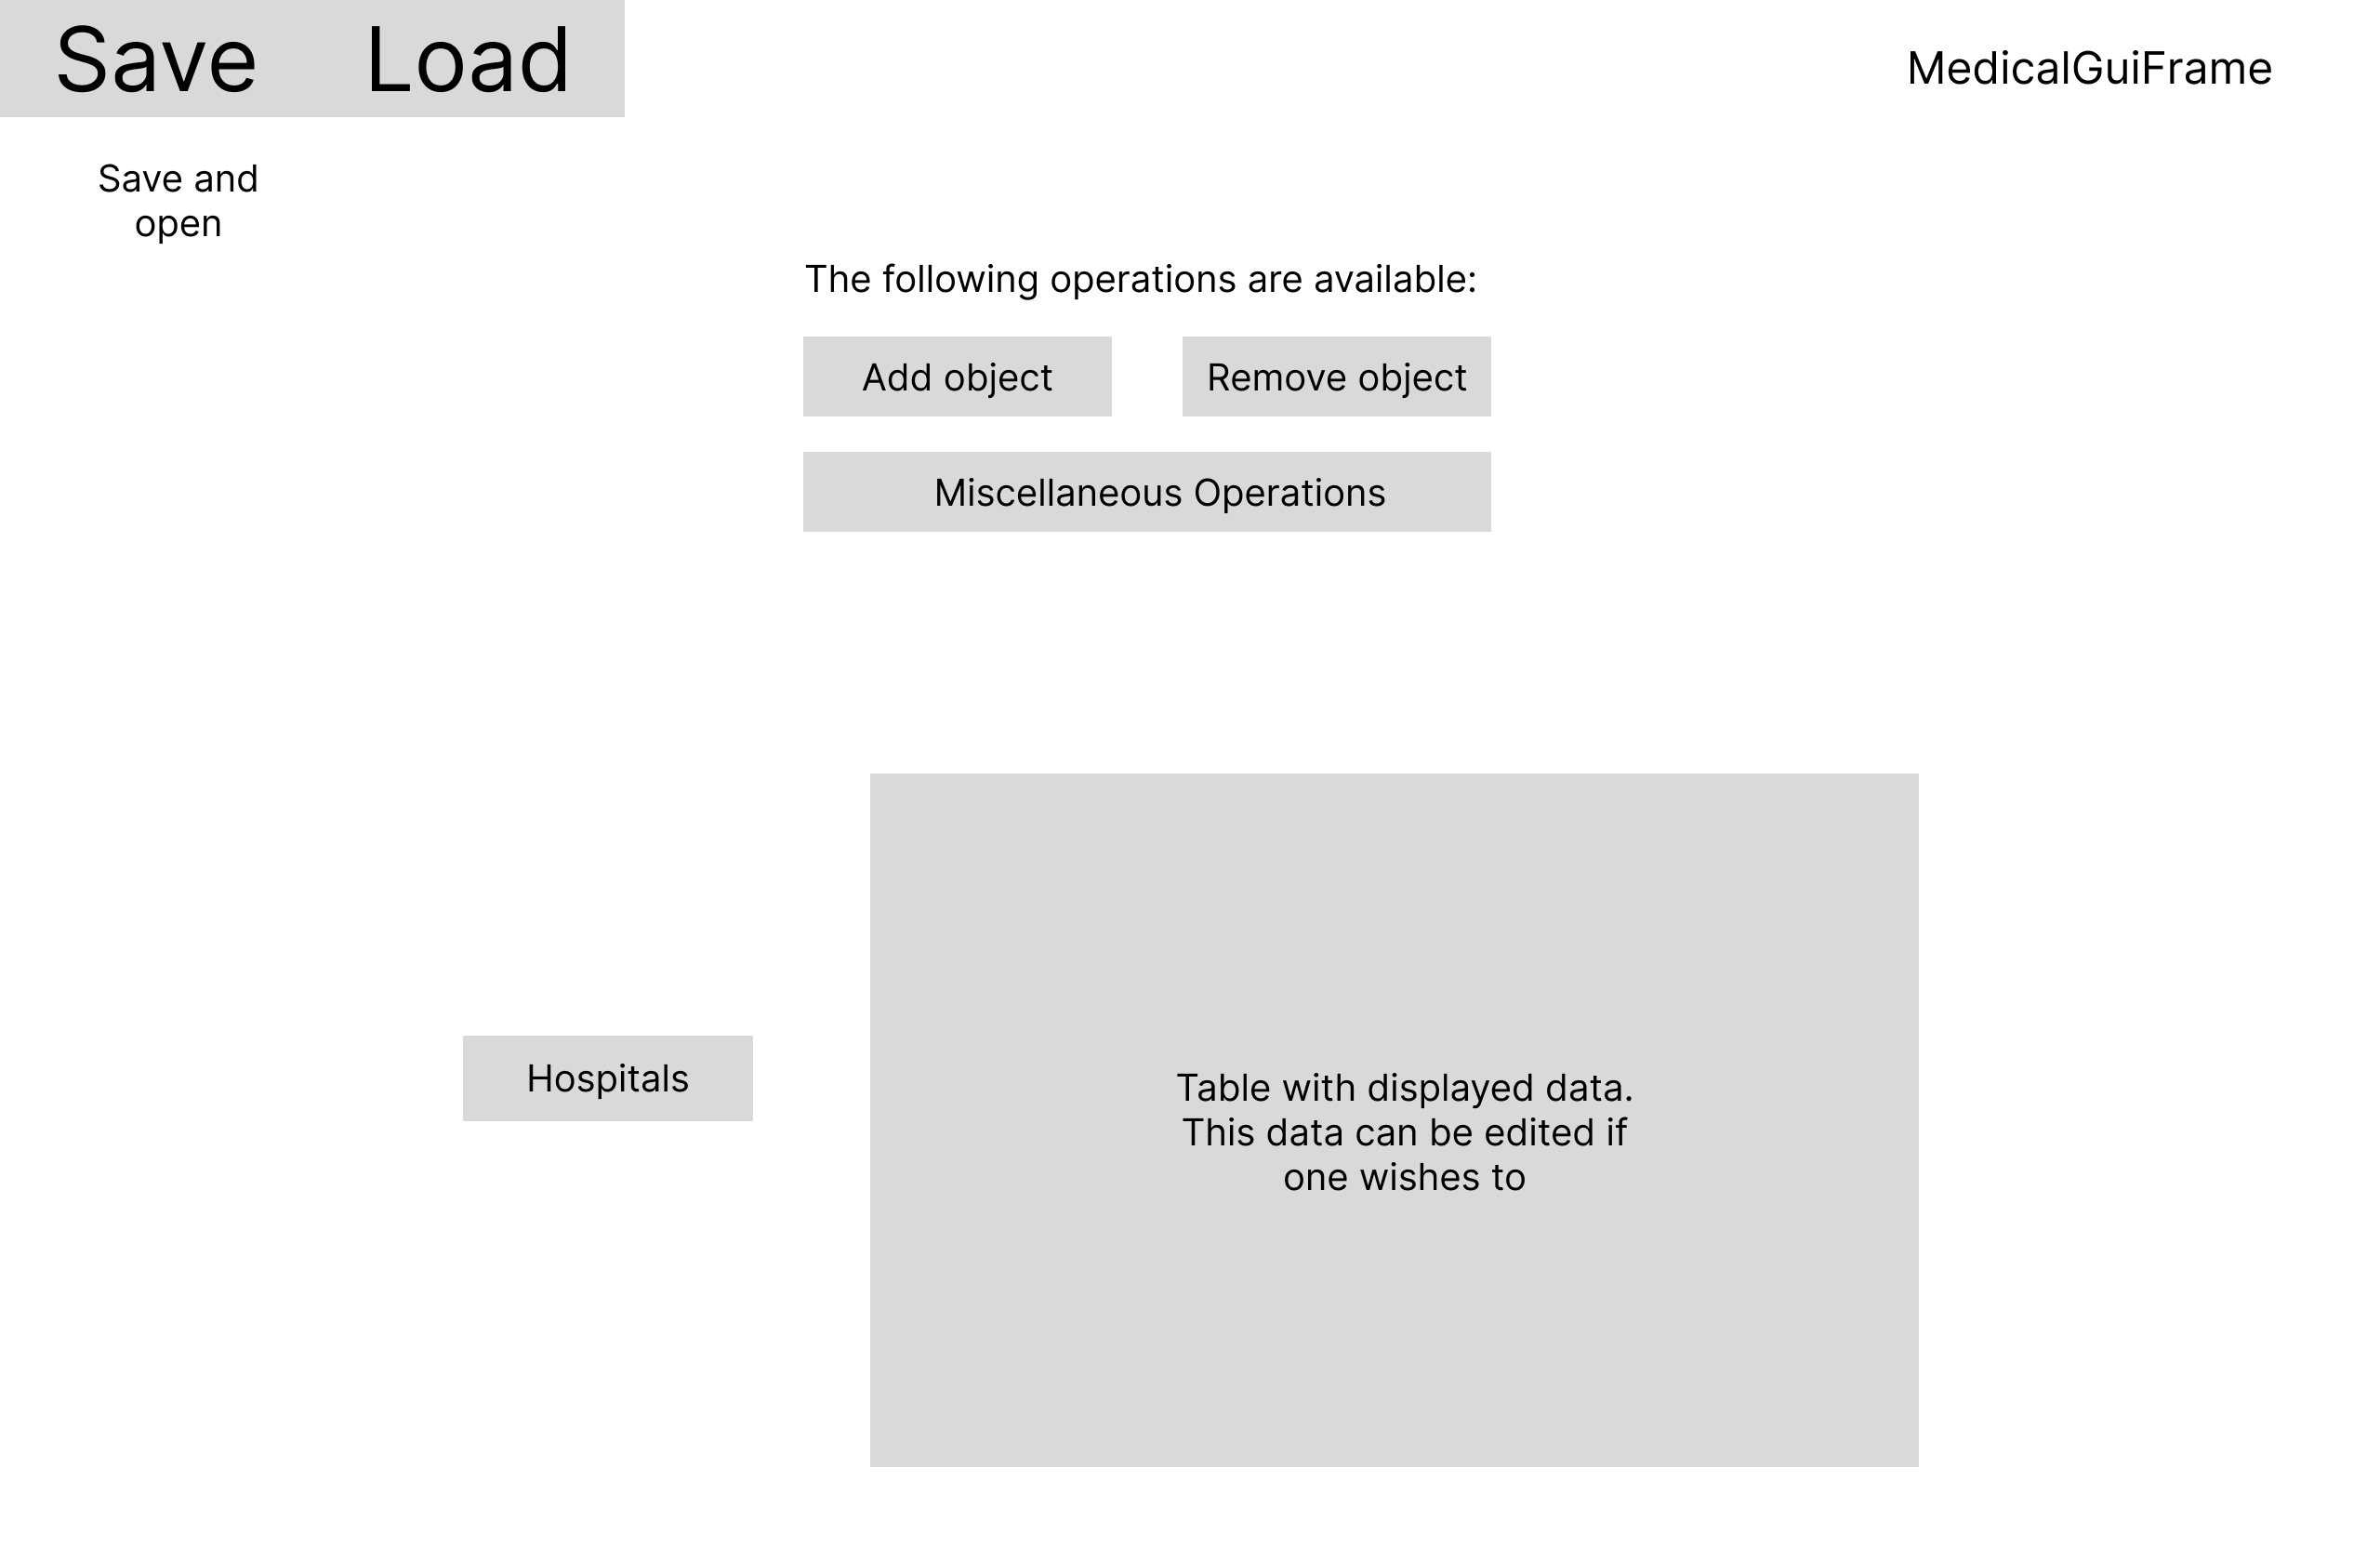
\includegraphics[width=0.95\textwidth]{./figures/Interface_designs/MedicalGuiFrame.png}
  \end{center}
\end{figure}

\begin{figure}
  \begin{center}
    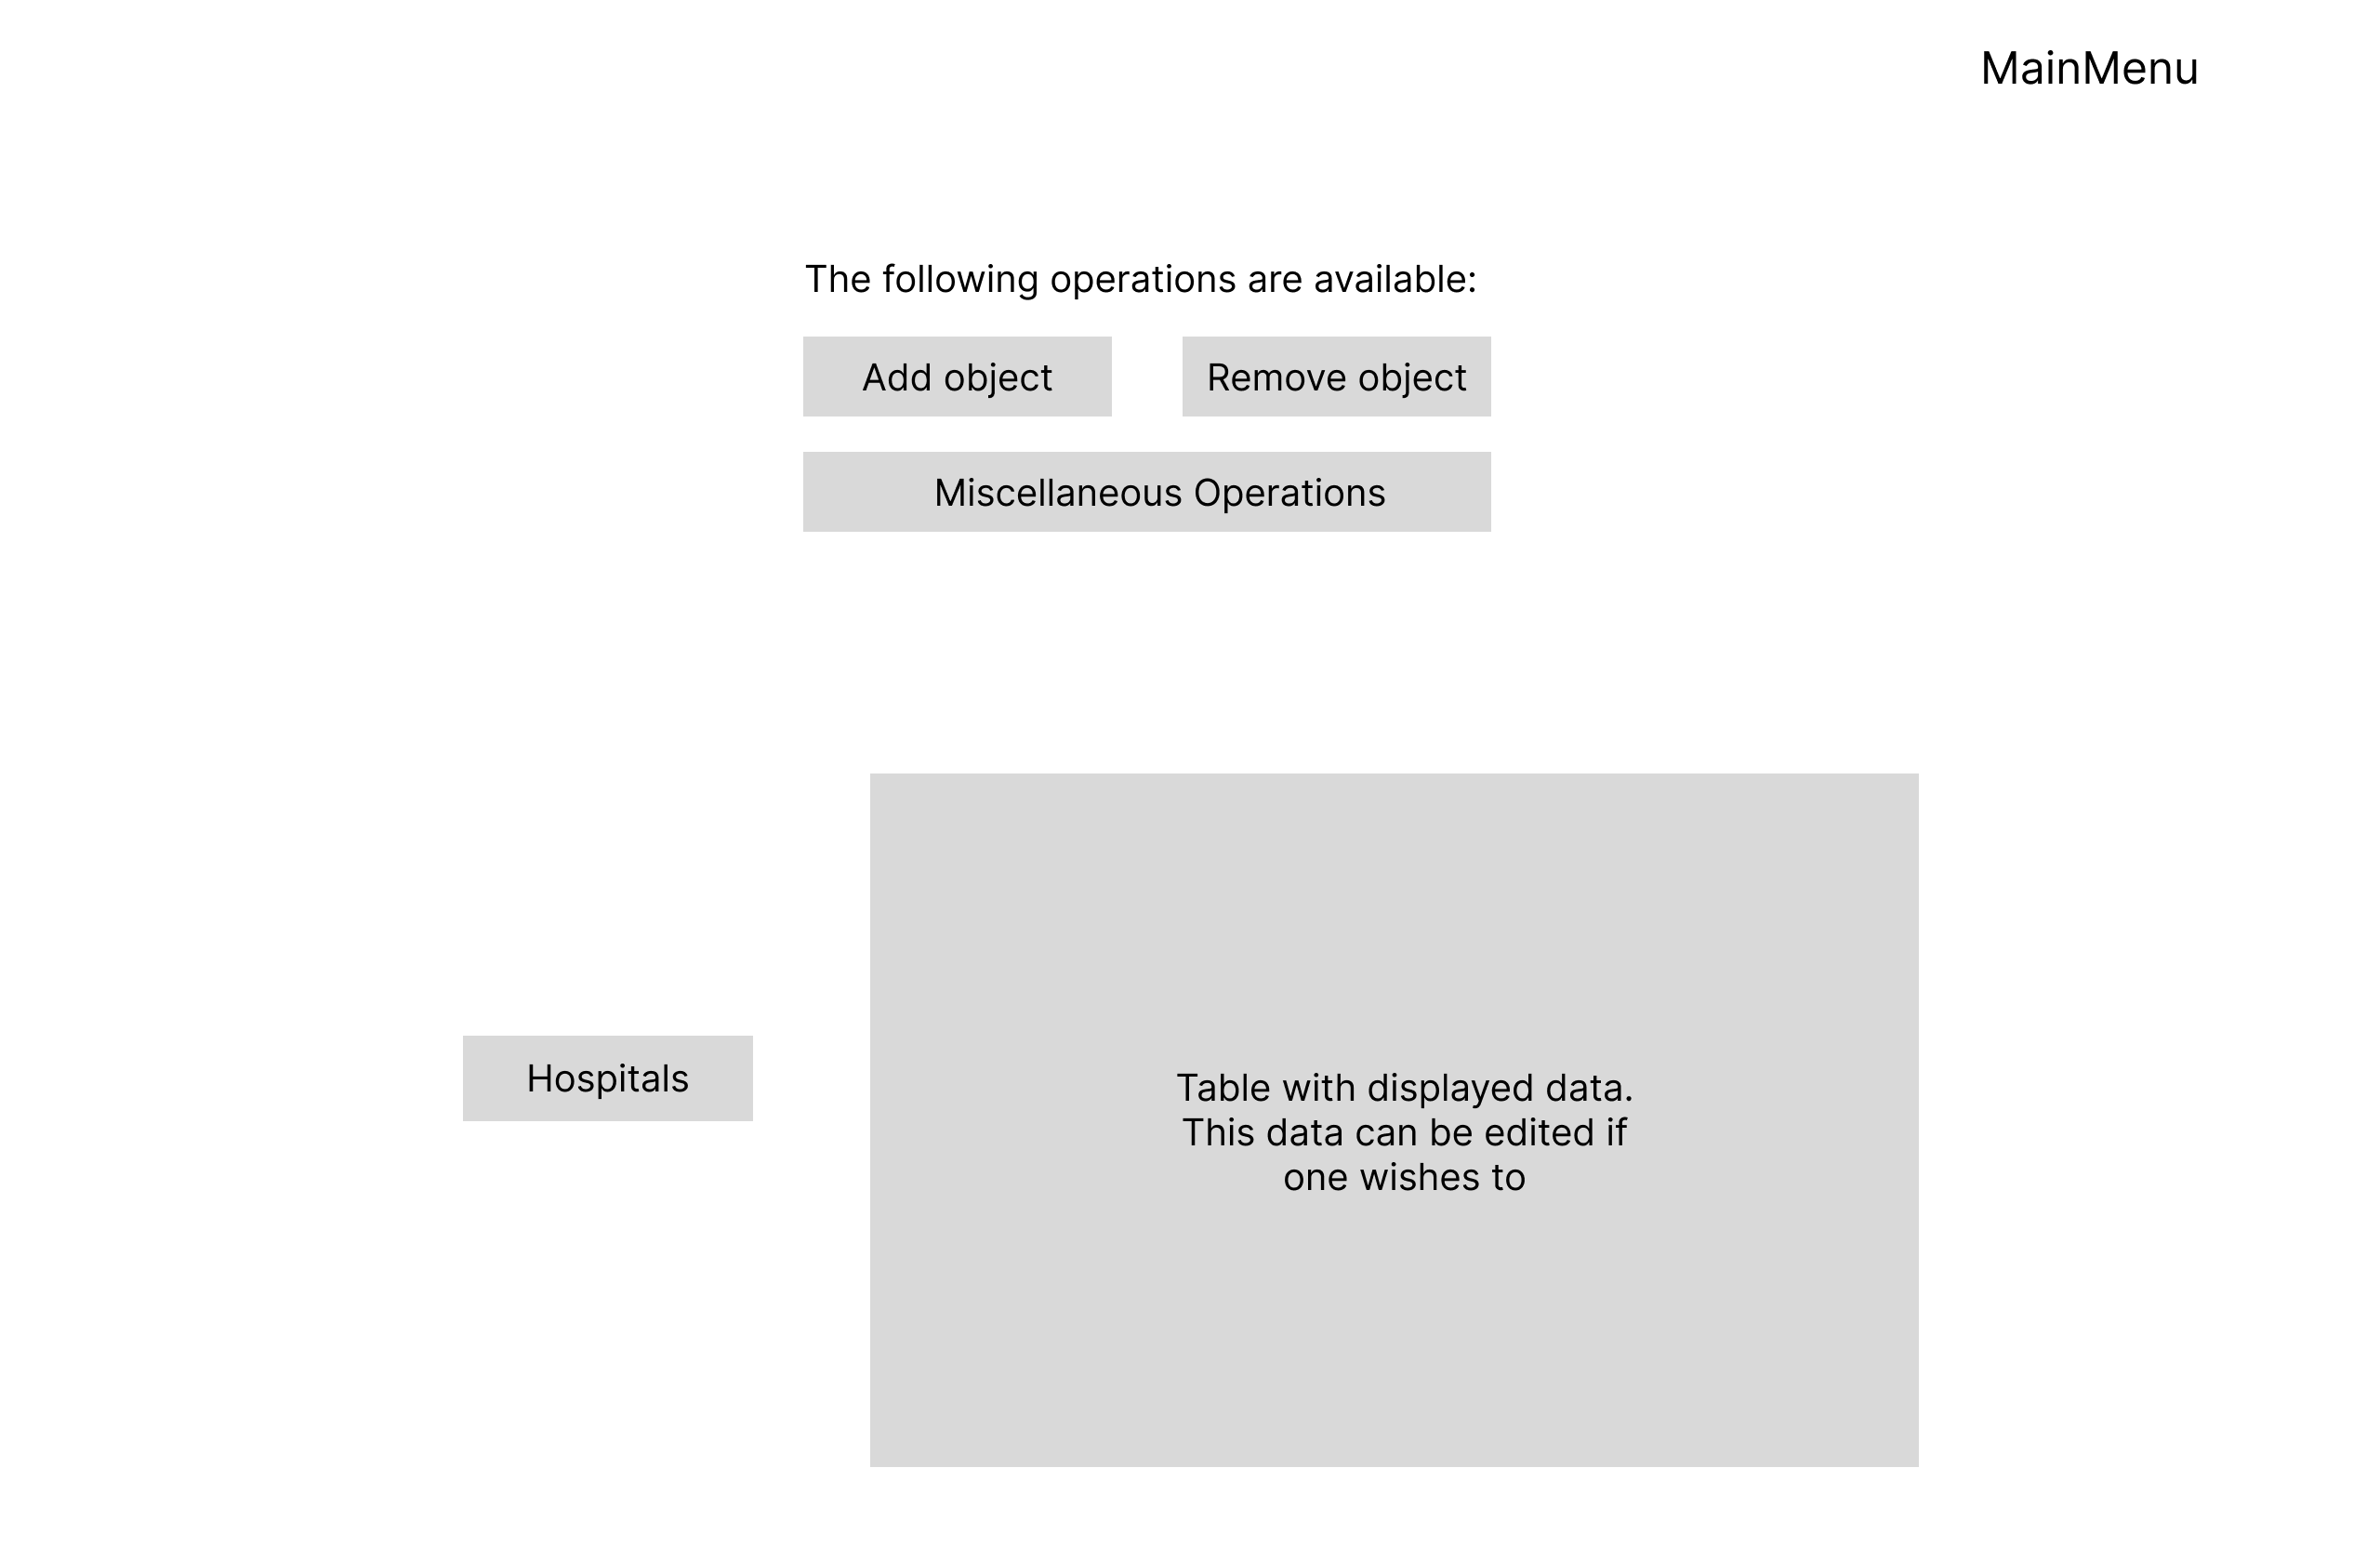
\includegraphics[width=0.95\textwidth]{./figures/Interface_designs/MainMenu.png}
  \end{center}
\end{figure}

\begin{figure}
  \begin{center}
    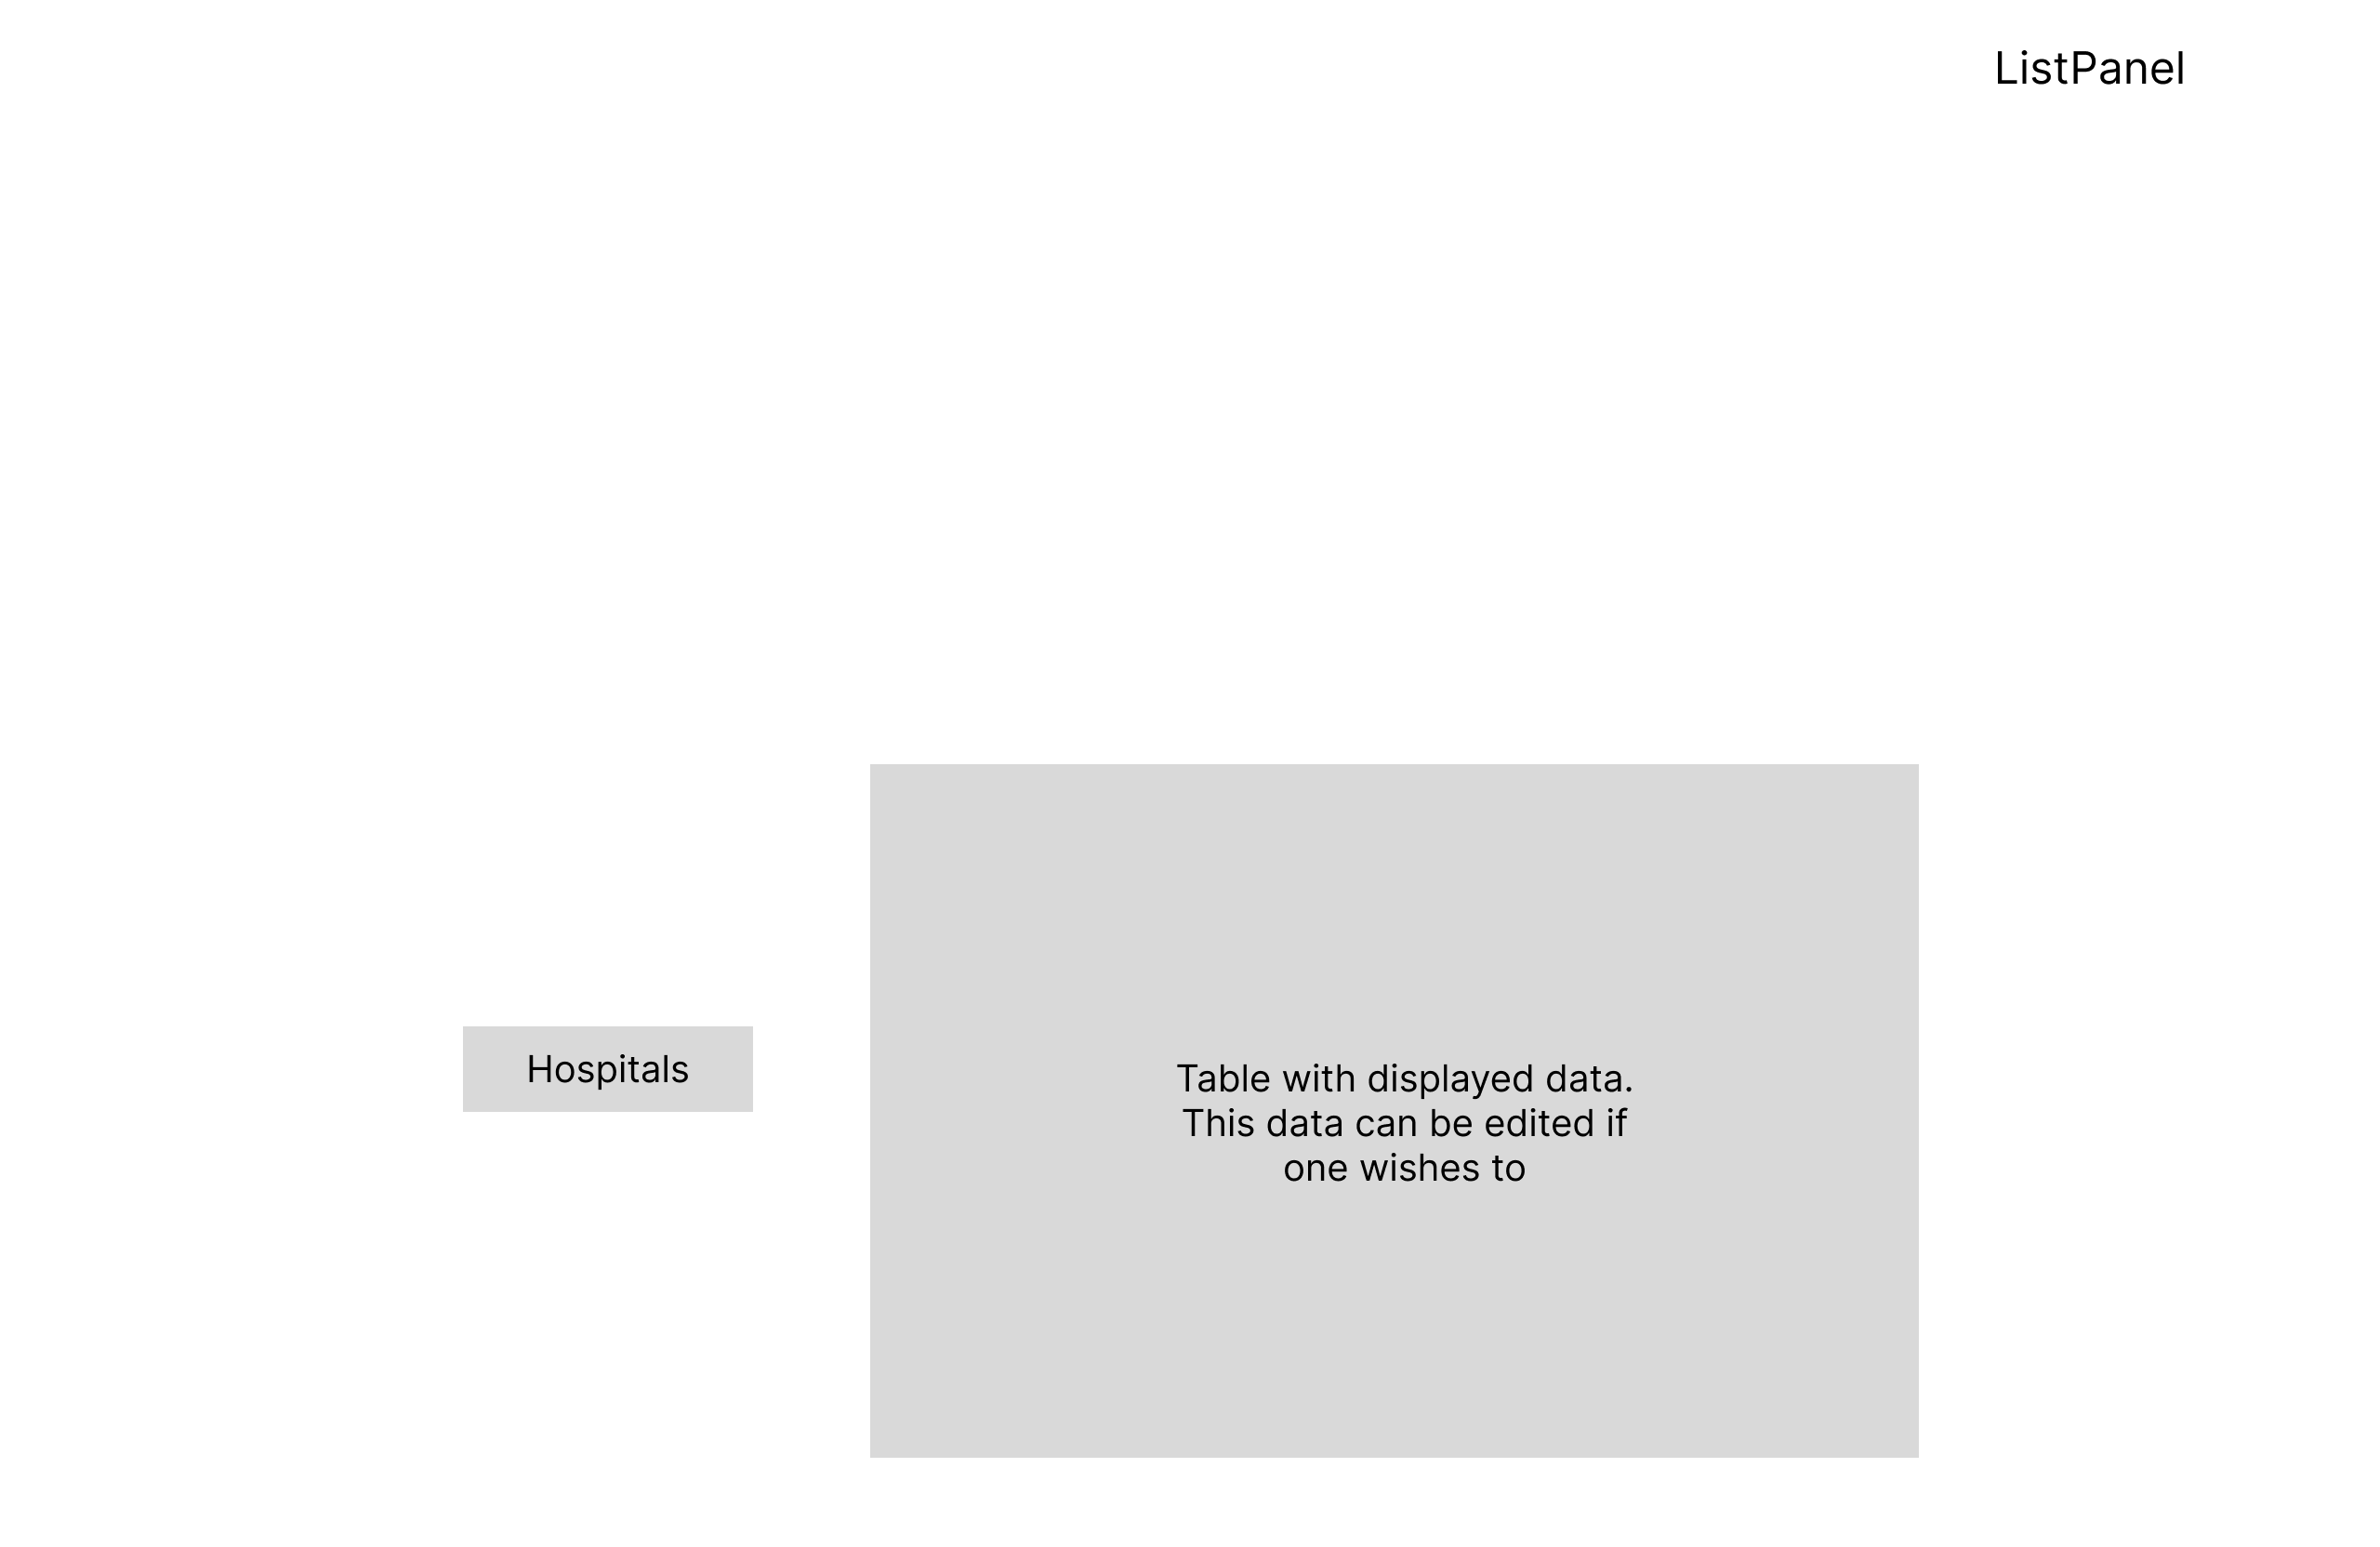
\includegraphics[width=0.95\textwidth]{./figures/Interface_designs/ListPanel.png}
  \end{center}
\end{figure}

\begin{figure}
  \begin{center}
    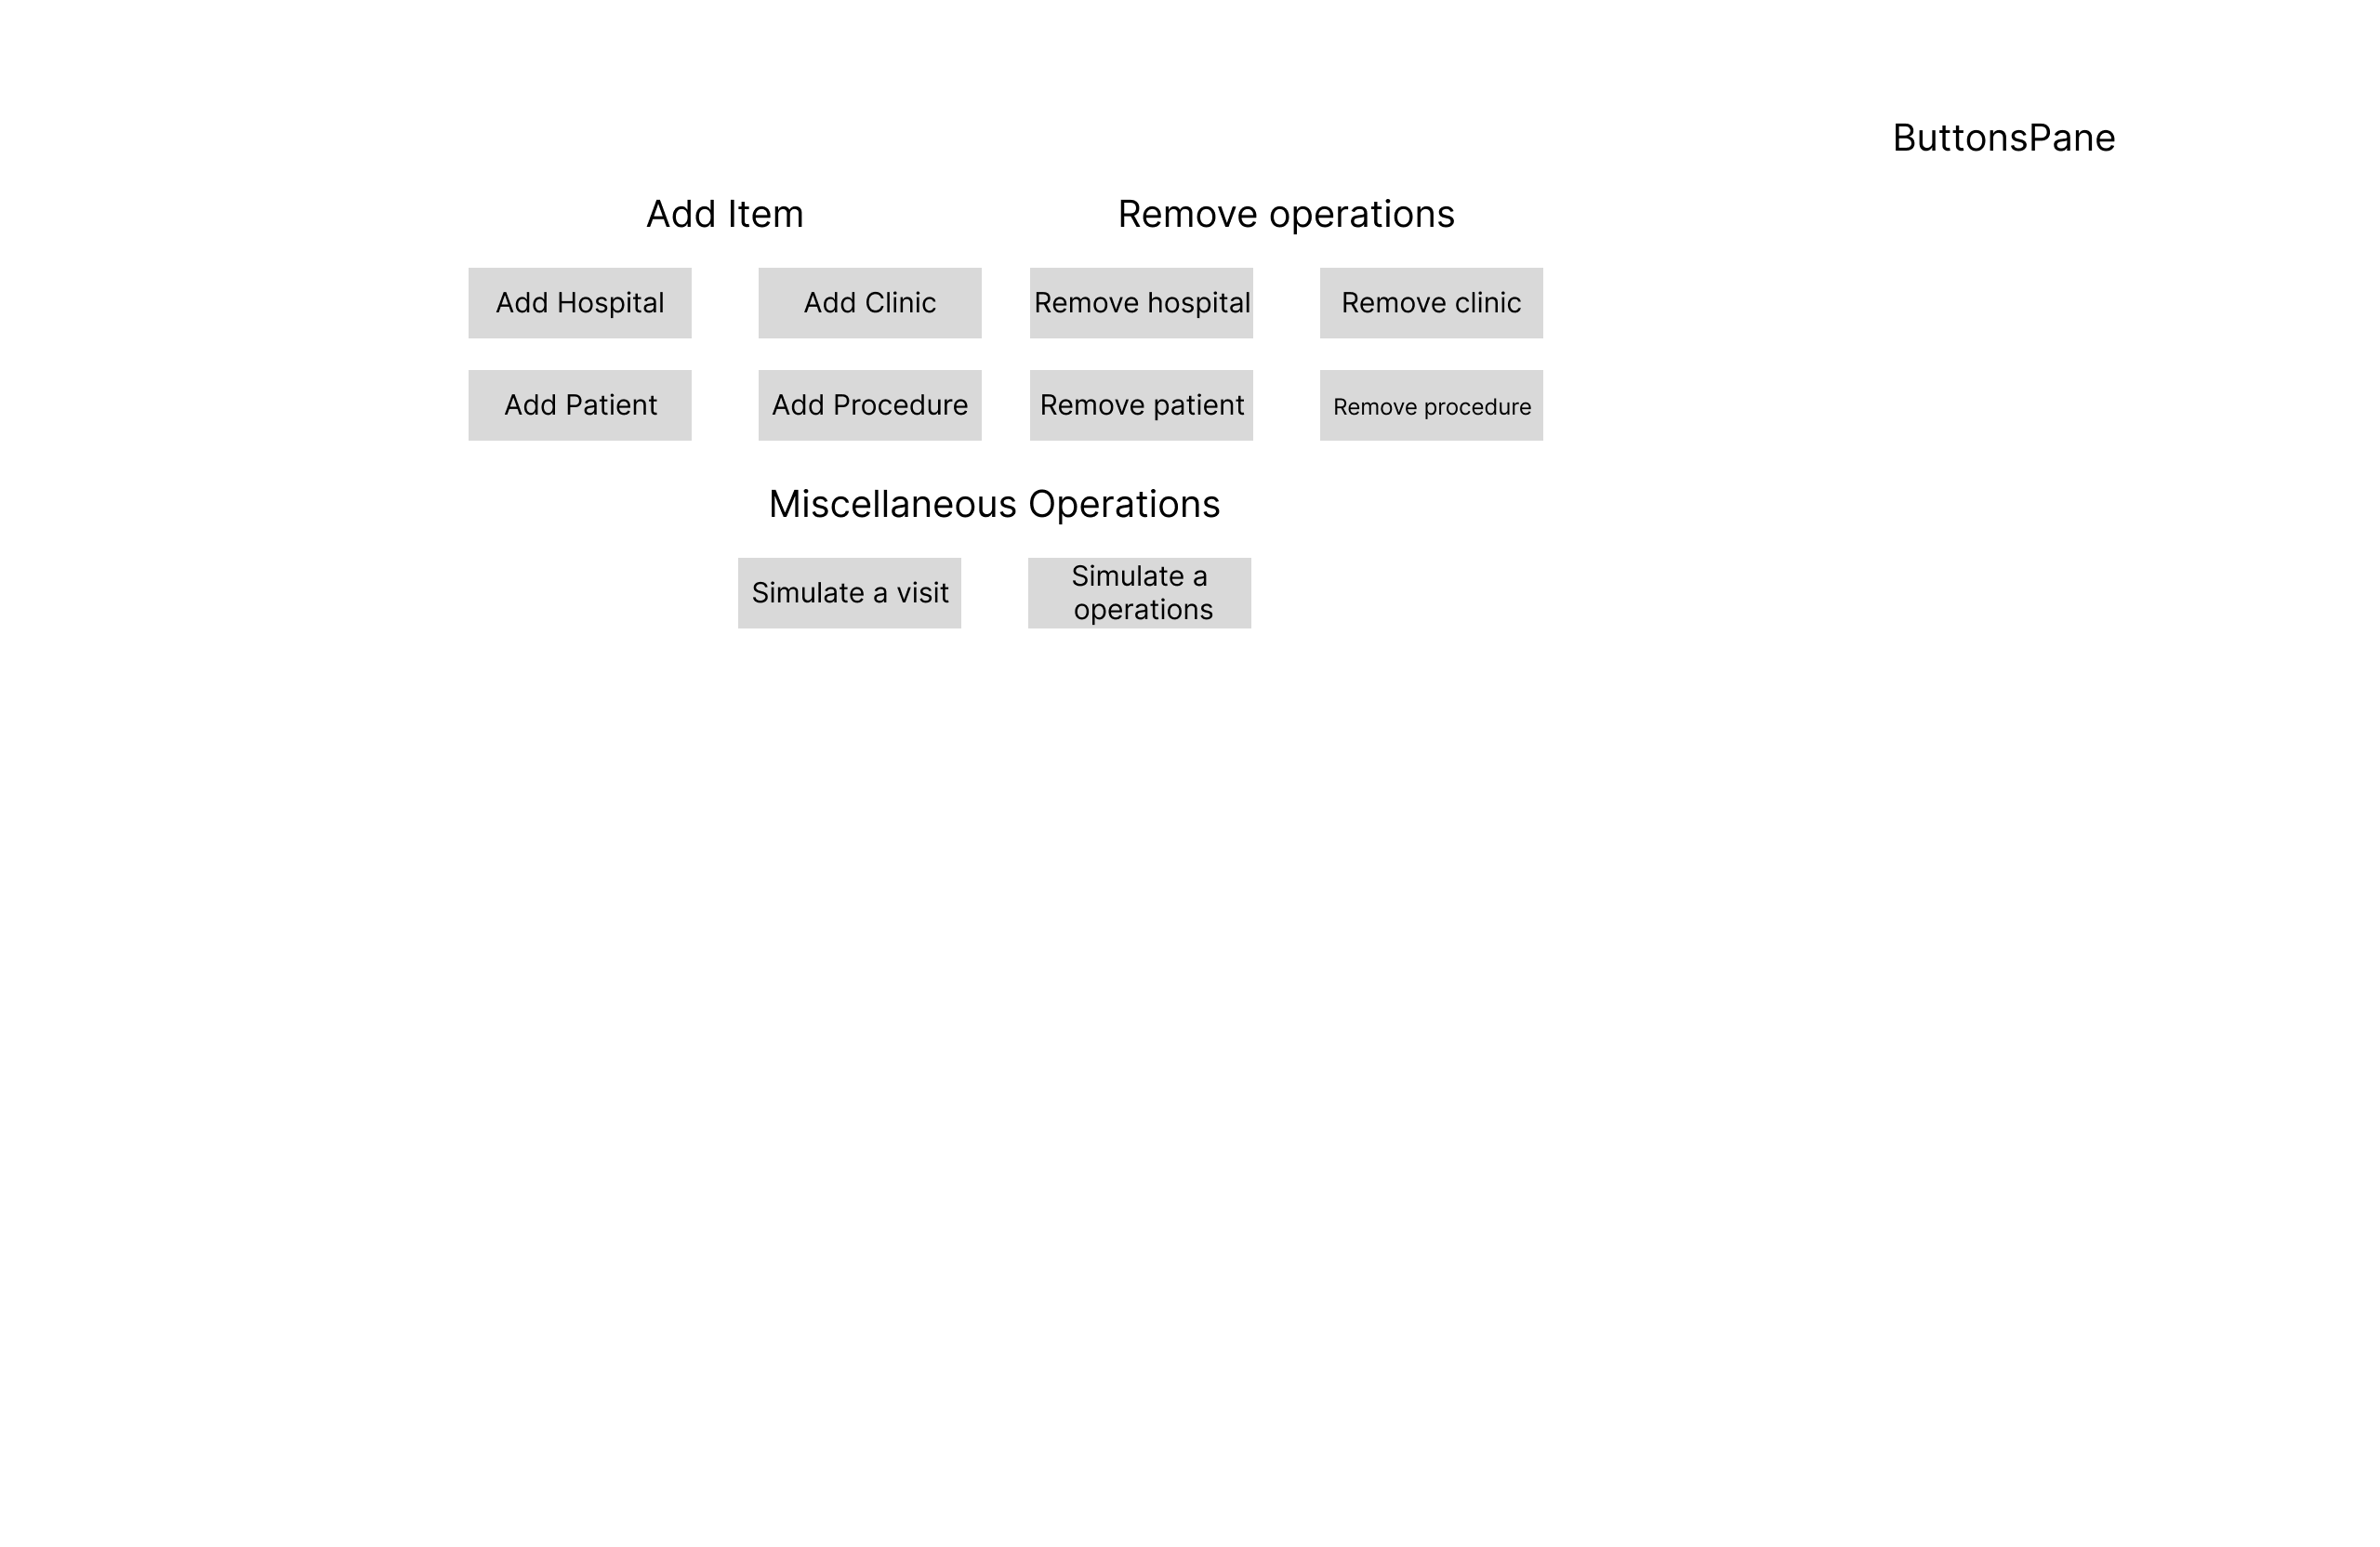
\includegraphics[width=0.95\textwidth]{./figures/Interface_designs/ButtonsPanel.png}
  \end{center}
\end{figure}

\begin{figure}
  \begin{center}
    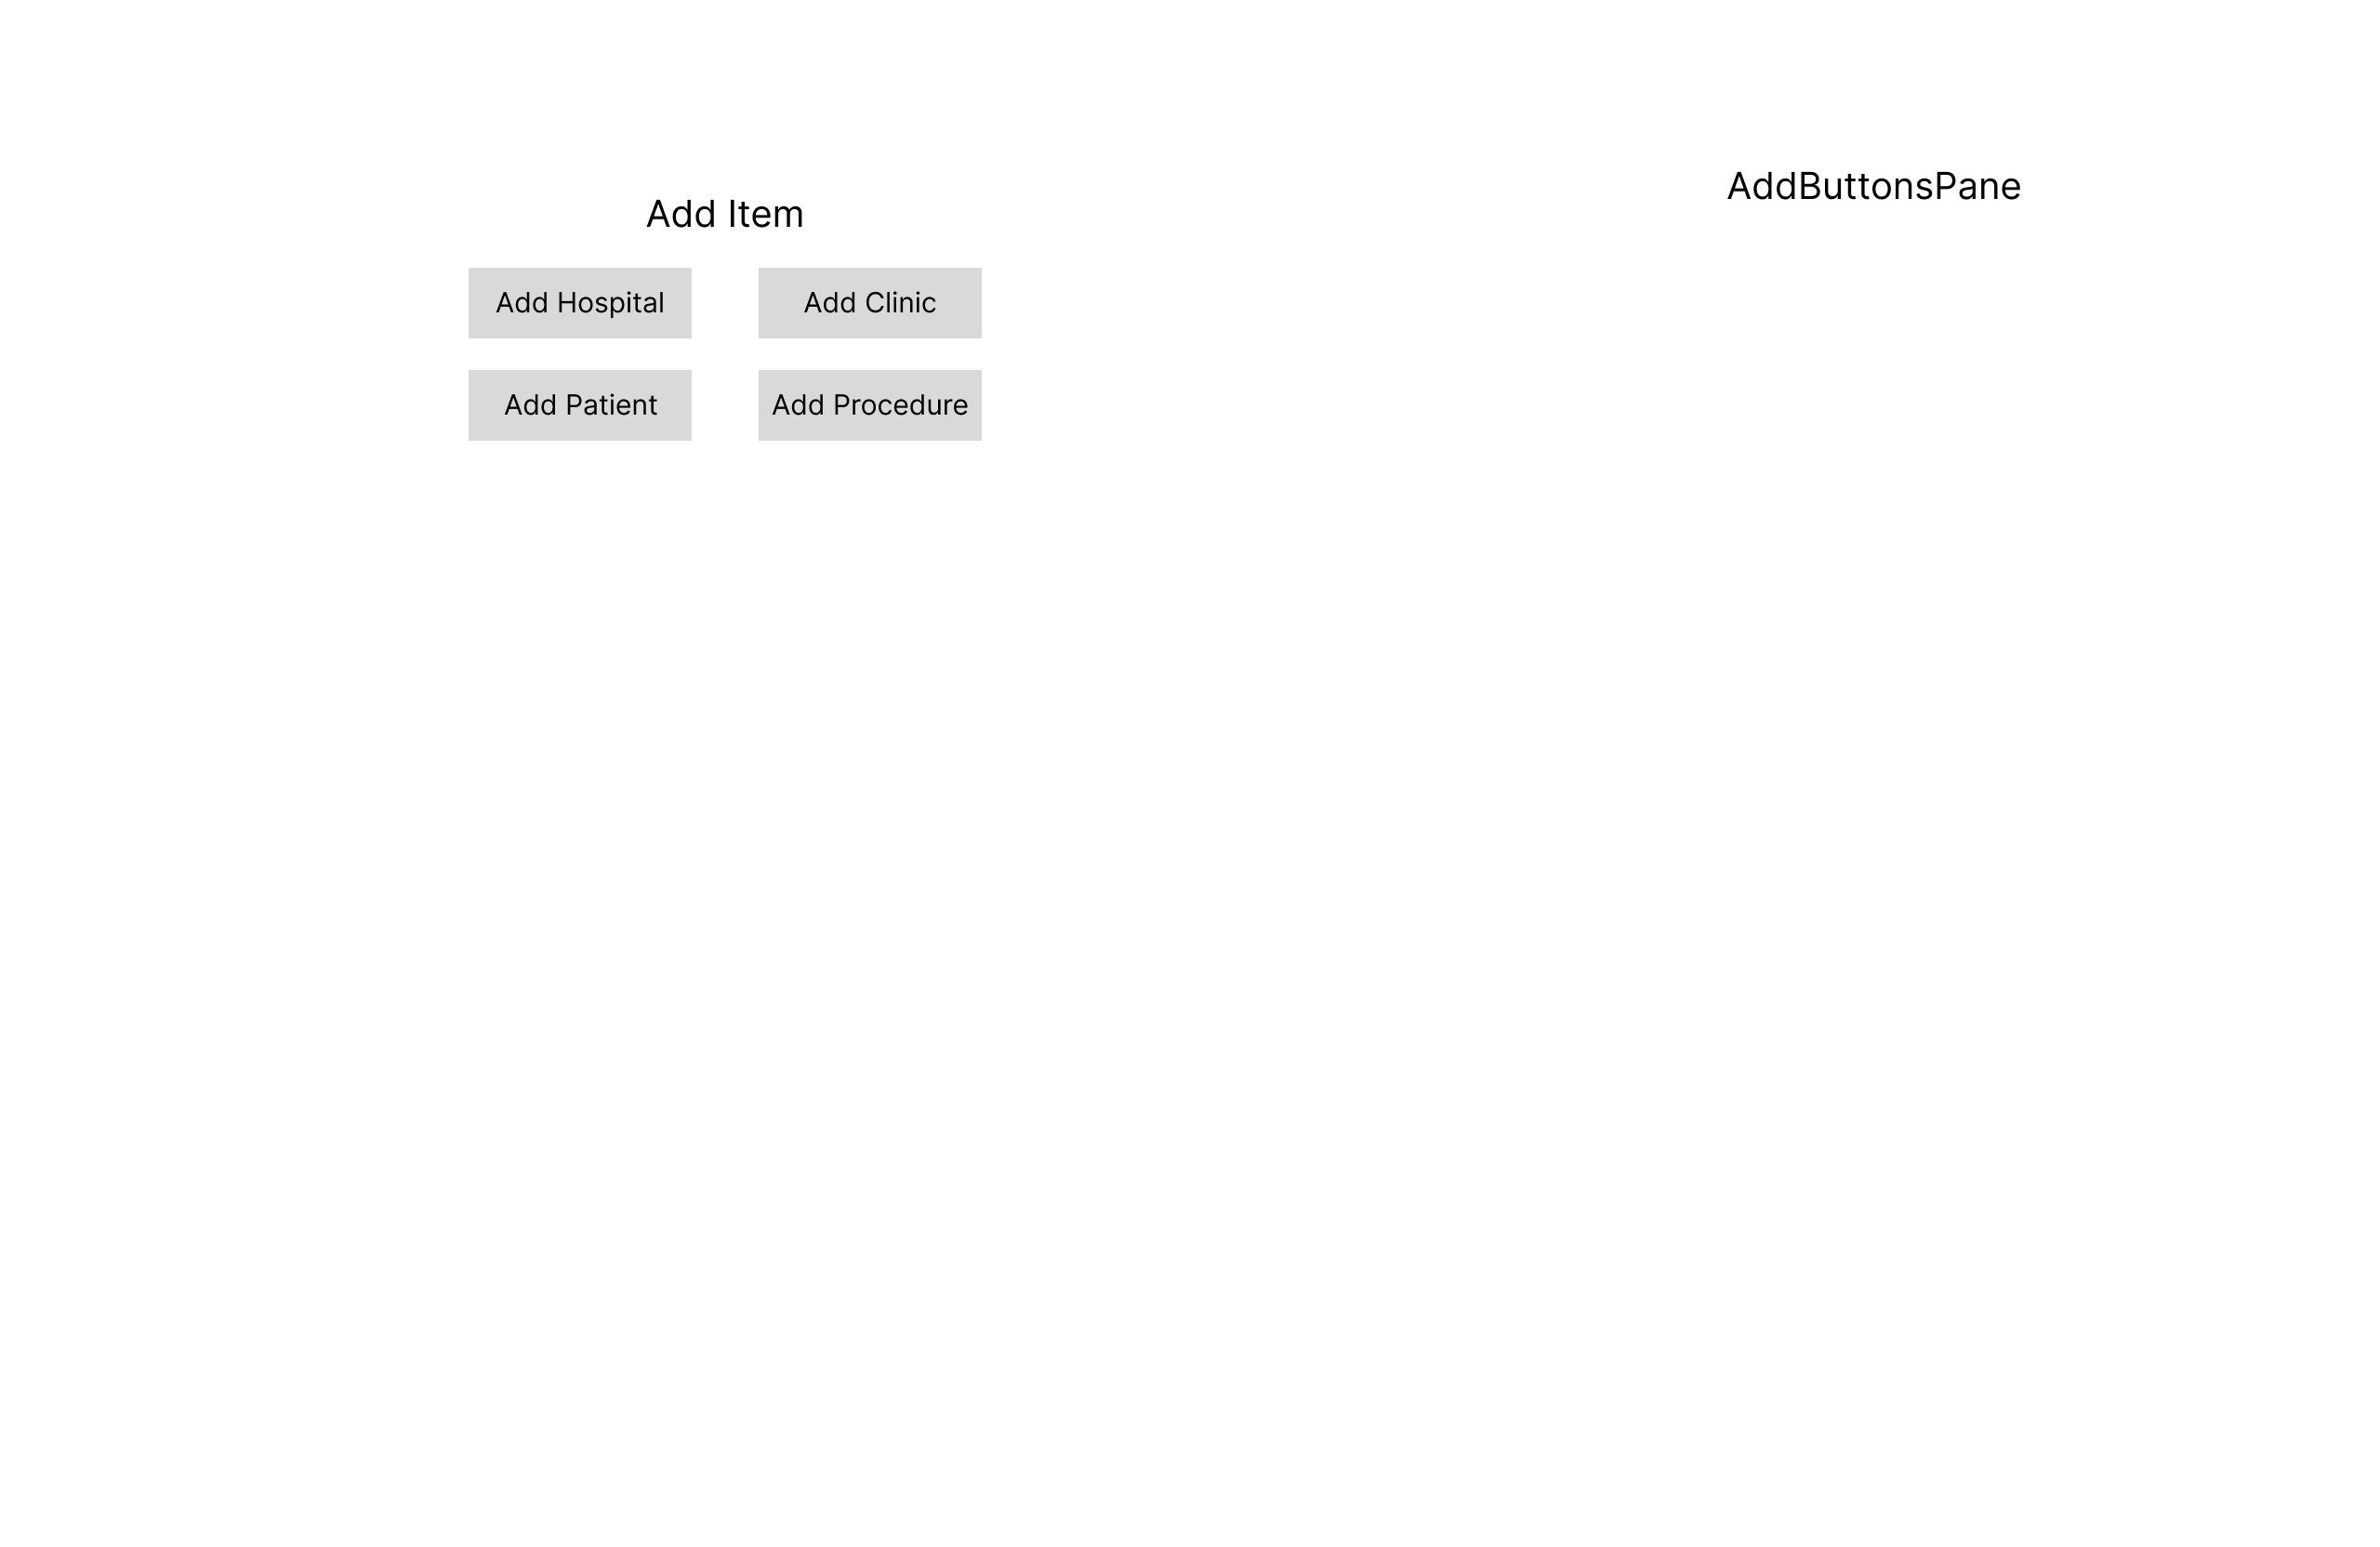
\includegraphics[width=0.95\textwidth]{./figures/Interface_designs/AddButtonsPanel.png}
  \end{center}
\end{figure}

\begin{figure}
  \begin{center}
    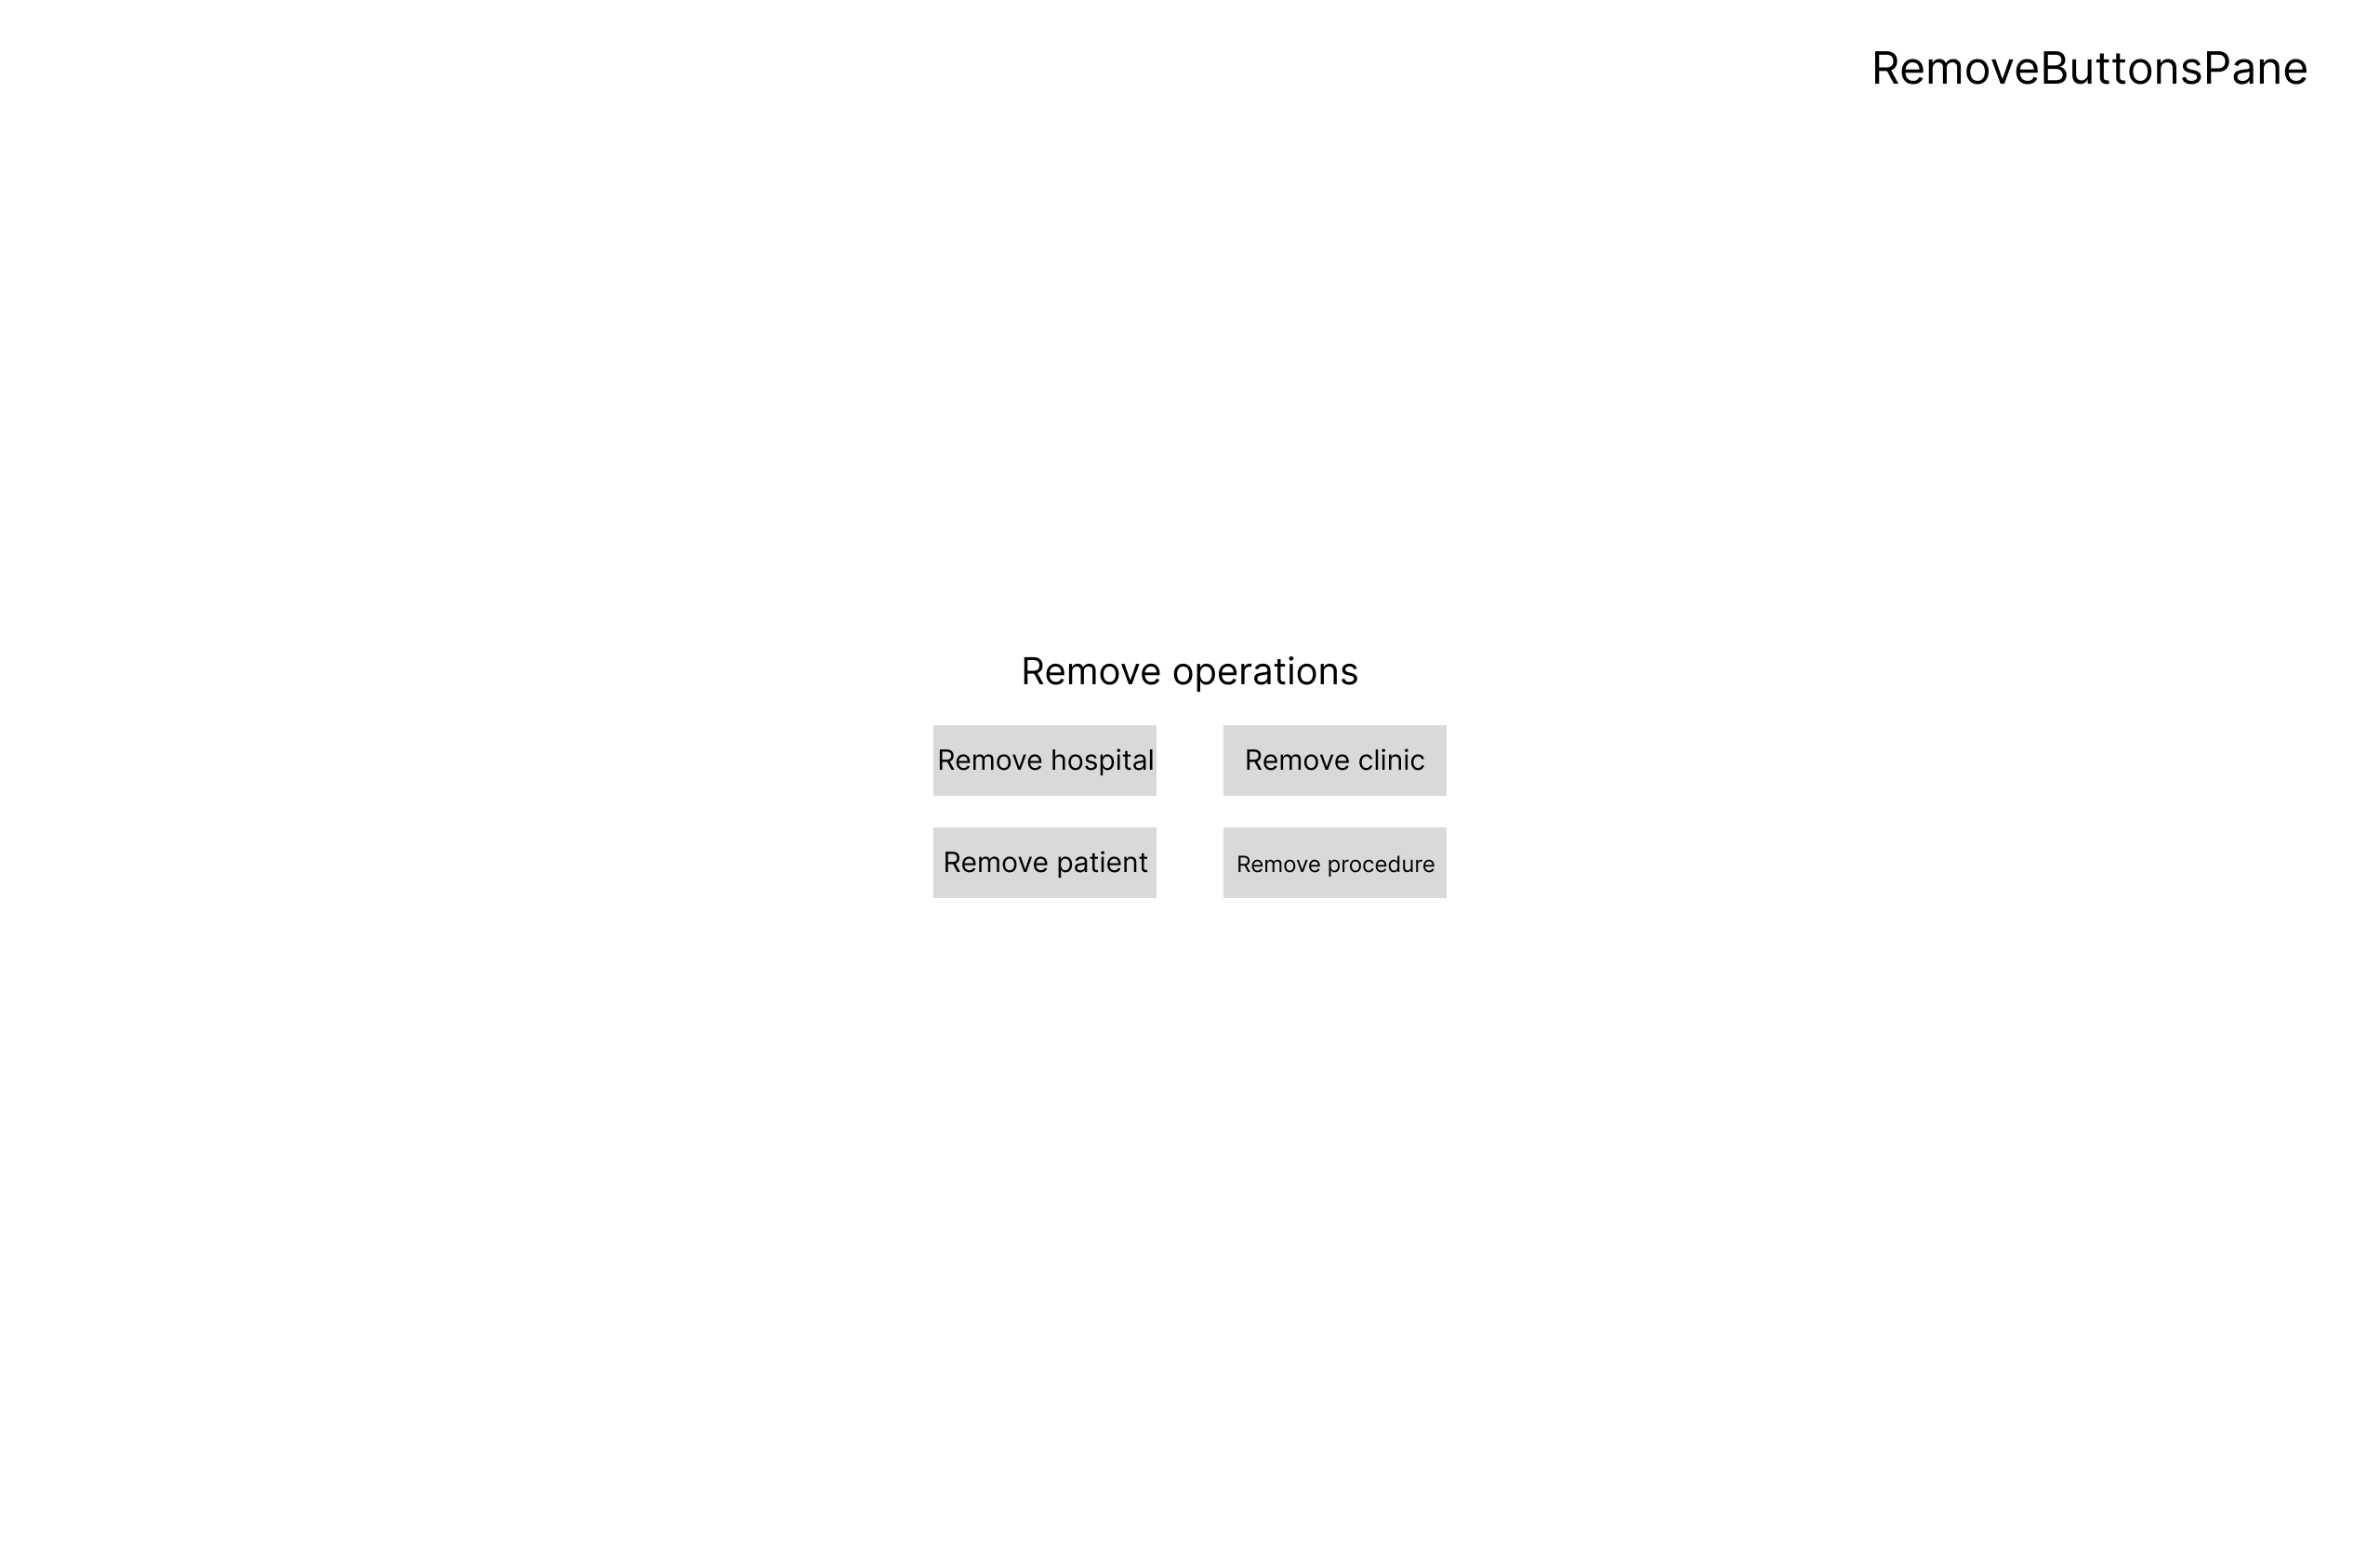
\includegraphics[width=0.95\textwidth]{./figures/Interface_designs/RemoveButtonsPanel.png}
  \end{center}
\end{figure}

\begin{figure}
  \begin{center}
    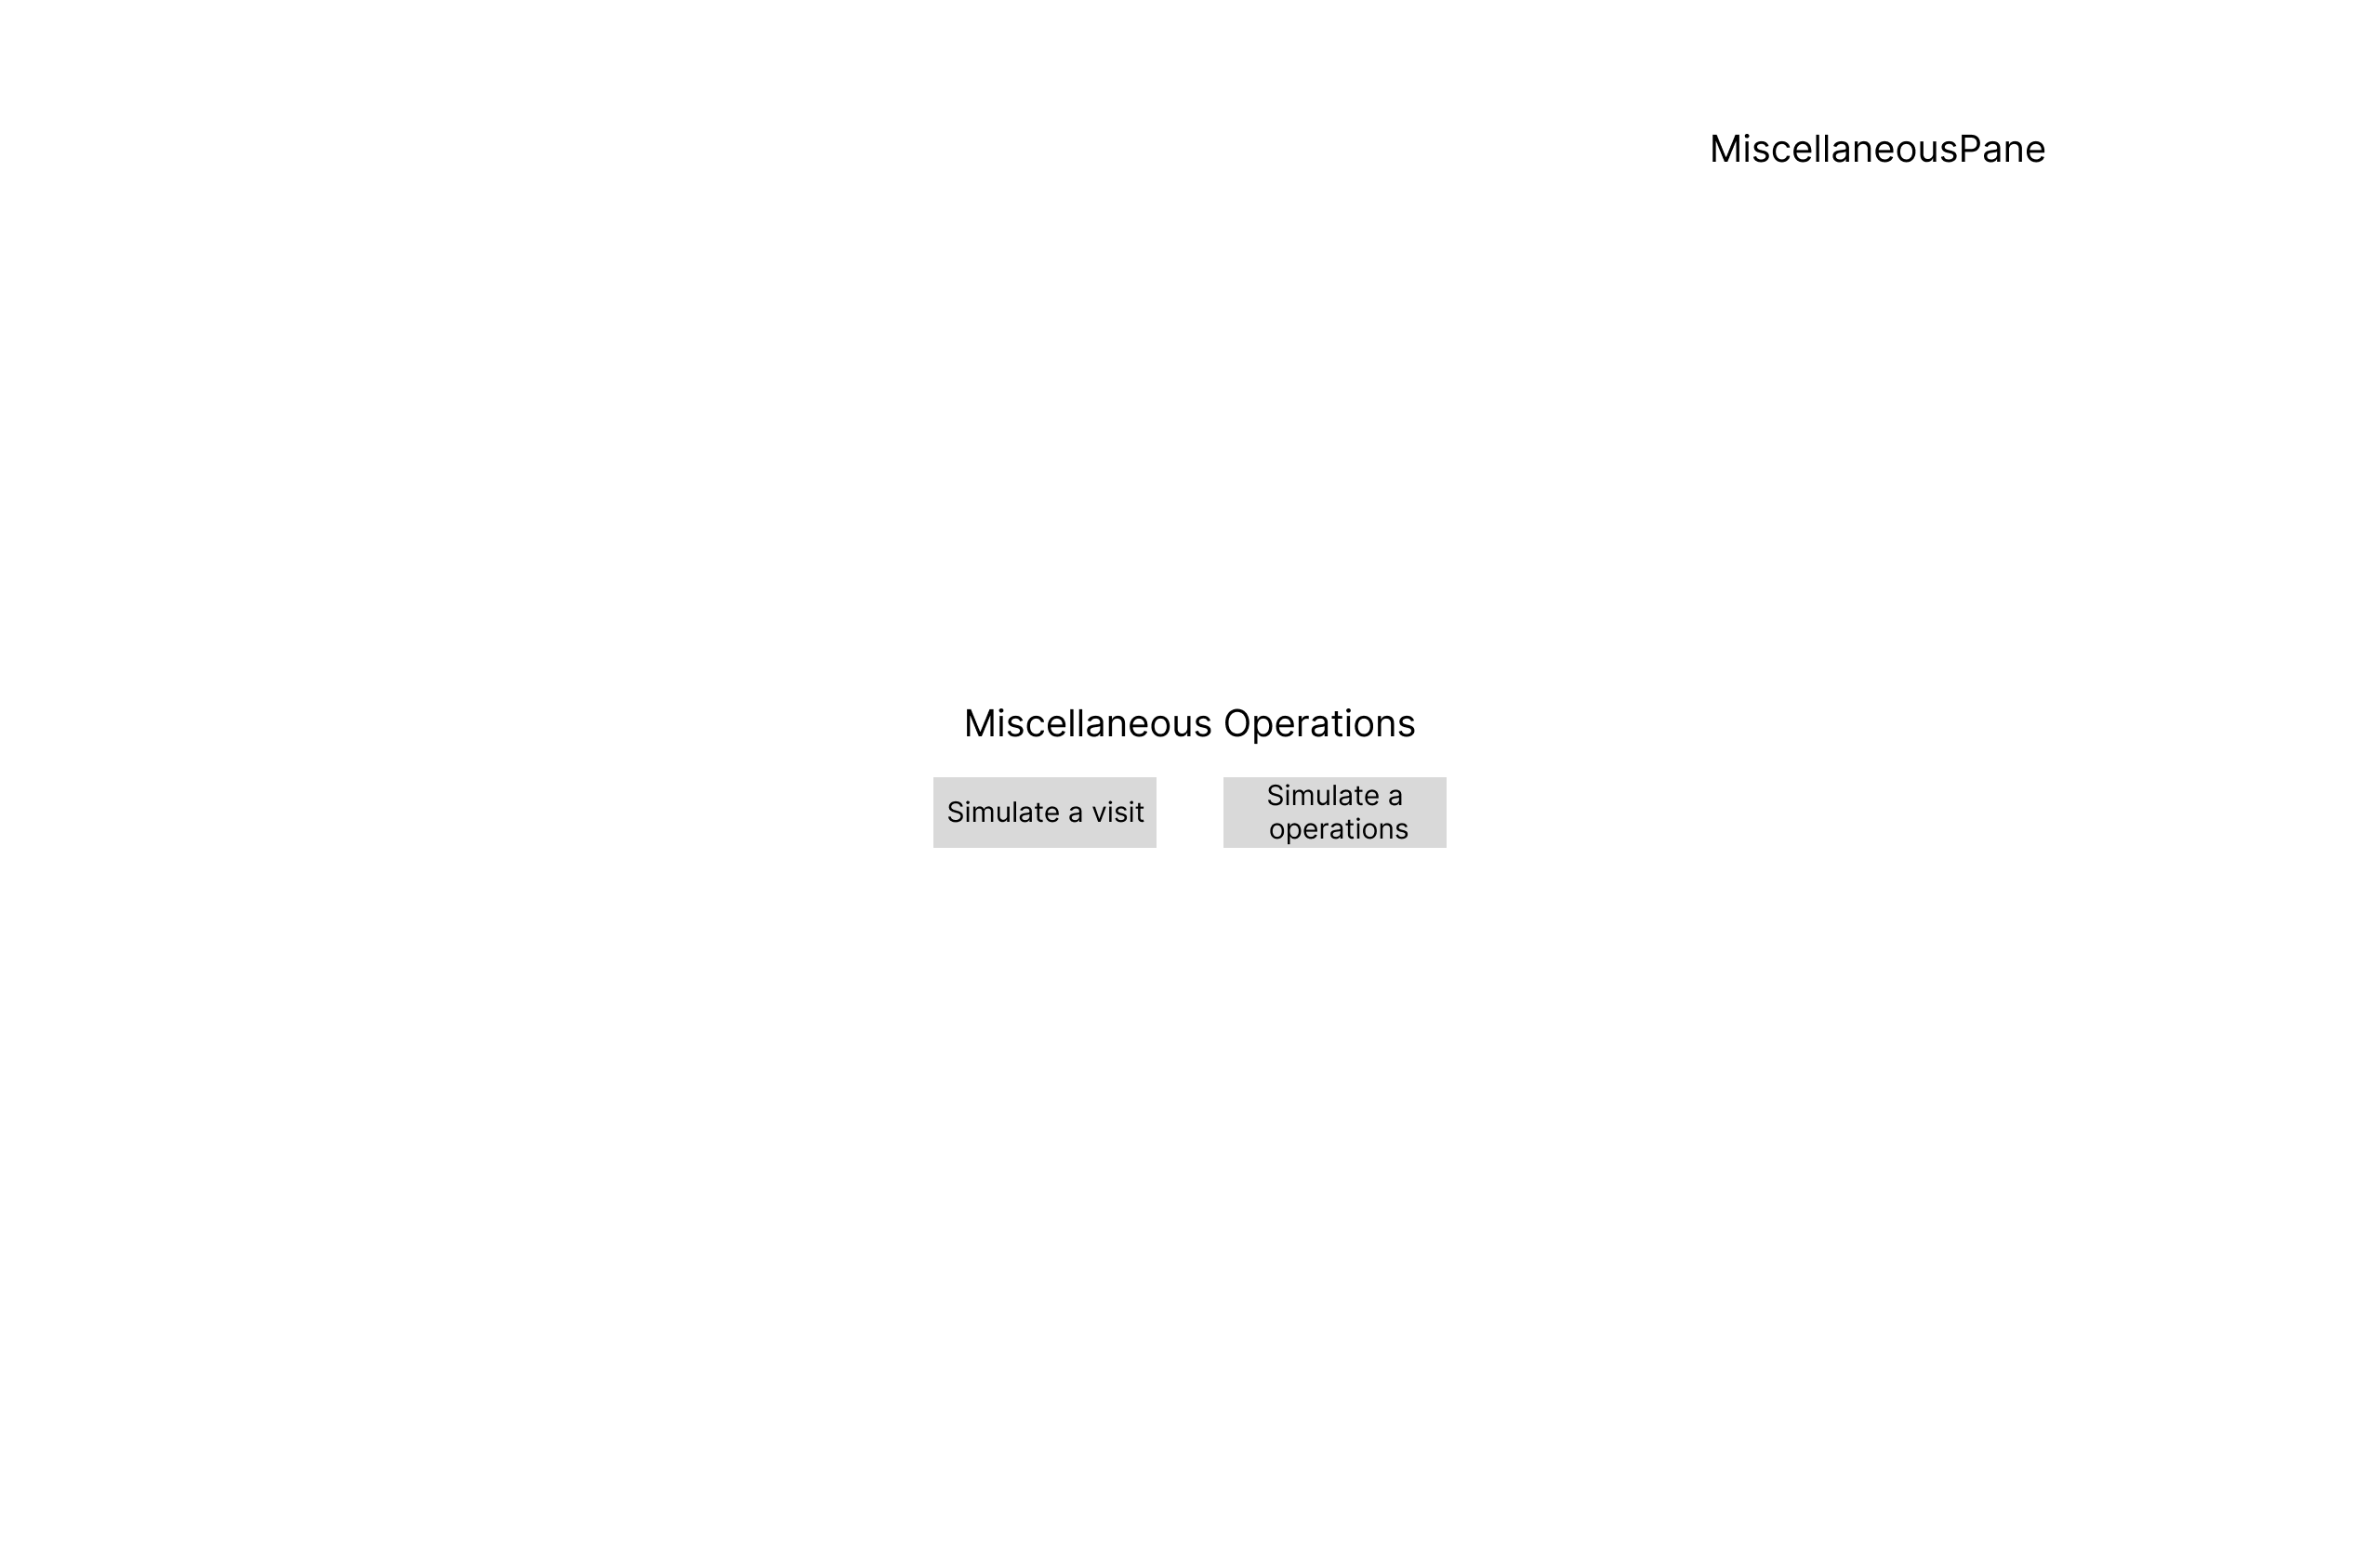
\includegraphics[width=0.95\textwidth]{./figures/Interface_designs/MiscellaneousPanel.png}
  \end{center}
\end{figure}

\newpage

\section{UML diagram}
The following diagram shows all the classes of this application, and their relations with both one another and the problem domain classes.
\begin{figure}[ht]
  \begin{center}
    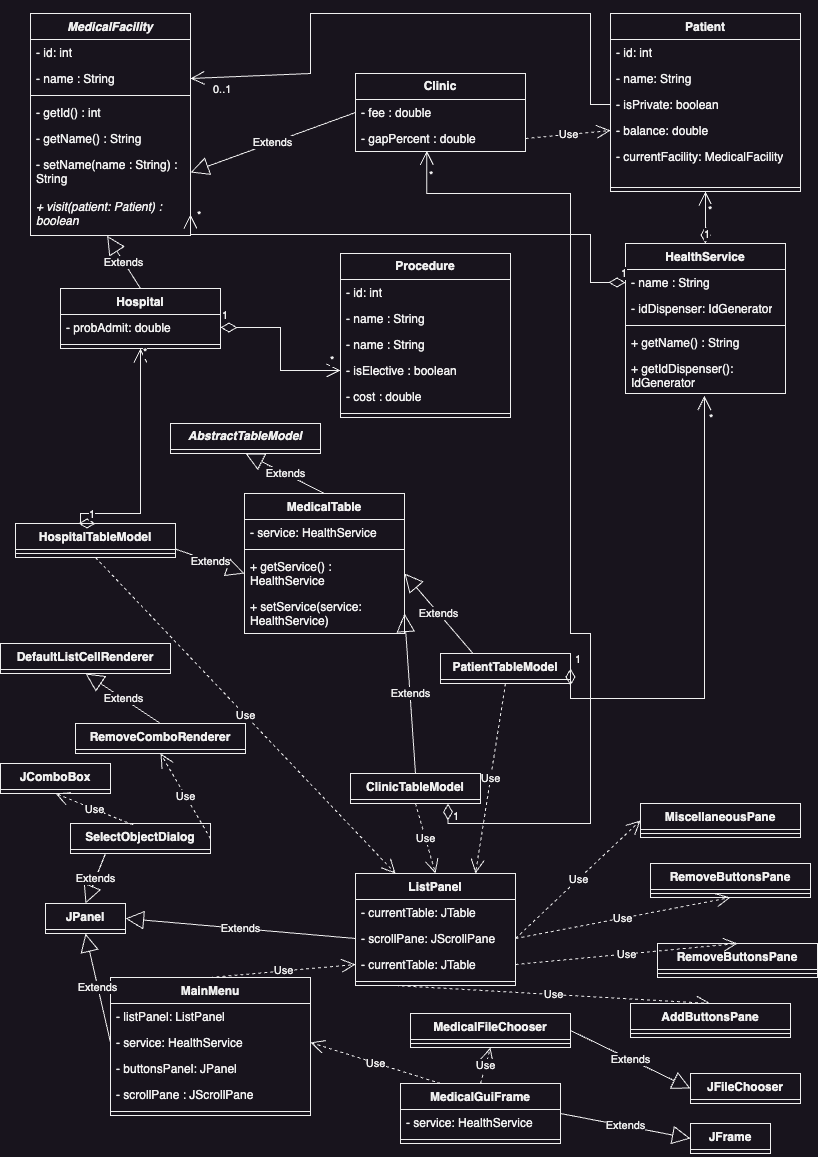
\includegraphics[width=0.95\textwidth]{figures/UML_diagram.png}
  \end{center}
\end{figure}

\newpage

\section{Source code}%
\label{sec:source_code}
The source code for this assignment can be found below, and it is divided in sections like so:
\begin{itemize}
  \item Components
  \item Models
\end{itemize}

\subsection{Components}\label{subsec:components} % (fold)
\textit{MedicalGui.java}\label{MedicalGui.java}
\inputminted{java}{./src/main/java/com/yvesstraten/medicalconsolegui/MedicalGui.java}

\textit{MainMenu.java}
\inputminted{java}{./src/main/java/com/yvesstraten/medicalconsolegui/components/MainMenu.java}

\textit{MedicalGuiFrame.java}
\inputminted{java}{./src/main/java/com/yvesstraten/medicalconsolegui/components/MedicalGuiFrame.java}

\textit{AddButtonsPane.java}
\inputminted{java}{./src/main/java/com/yvesstraten/medicalconsolegui/components/AddButtonsPane.java}

\textit{MiscellaneousPane.java}
\inputminted{java}{./src/main/java/com/yvesstraten/medicalconsolegui/components/MiscellaneousPane.java}

\textit{RemoveComboRenderer.java}
\inputminted{java}{./src/main/java/com/yvesstraten/medicalconsolegui/RemoveComboRenderer.java}

\textit{RemoveButtonsPane.java}
\inputminted{java}{./src/main/java/com/yvesstraten/medicalconsolegui/components/RemoveButtonsPane.java}

\textit{MedicalFileChooser.java}
\inputminted{java}{./src/main/java/com/yvesstraten/medicalconsolegui/components/MedicalFileChooser.java}

\textit{SelectObjectDialog.java}
\inputminted{java}{./src/main/java/com/yvesstraten/medicalconsolegui/components/SelectObjectDialog.java}

\textit{ListPanel.java}
\inputminted{java}{./src/main/java/com/yvesstraten/medicalconsolegui/components/ListPanel.java}
% subsection Components (end)

\subsection{Models}\label{sec:models} % (fold)
\textit{ProcedureTableModel.java}
\inputminted{java}{./src/main/java/com/yvesstraten/medicalconsolegui/models/ProcedureTableModel.java}

\textit{MedicalTableModel.java}
\inputminted{java}{./src/main/java/com/yvesstraten/medicalconsolegui/models/MedicalTableModel.java}

\textit{HospitalTableModel.java}
\inputminted{java}{./src/main/java/com/yvesstraten/medicalconsolegui/models/HospitalTableModel.java}

\textit{PatientTableModel.java}
\inputminted{java}{./src/main/java/com/yvesstraten/medicalconsolegui/models/PatientTableModel.java}

\textit{ClinicTableModel.java}
\inputminted{java}{./src/main/java/com/yvesstraten/medicalconsolegui/models/ClinicTableModel.java}
% subsection Models (end)

\newpage 

\section{Runtime output}\label{sec:runtime_output} % (fold)
The following images showcase the output at runtime for the application, and its general, realized look.

\subsection{Adding}\label{sub:adding} % (fold)
\begin{figure}
  \begin{center}
    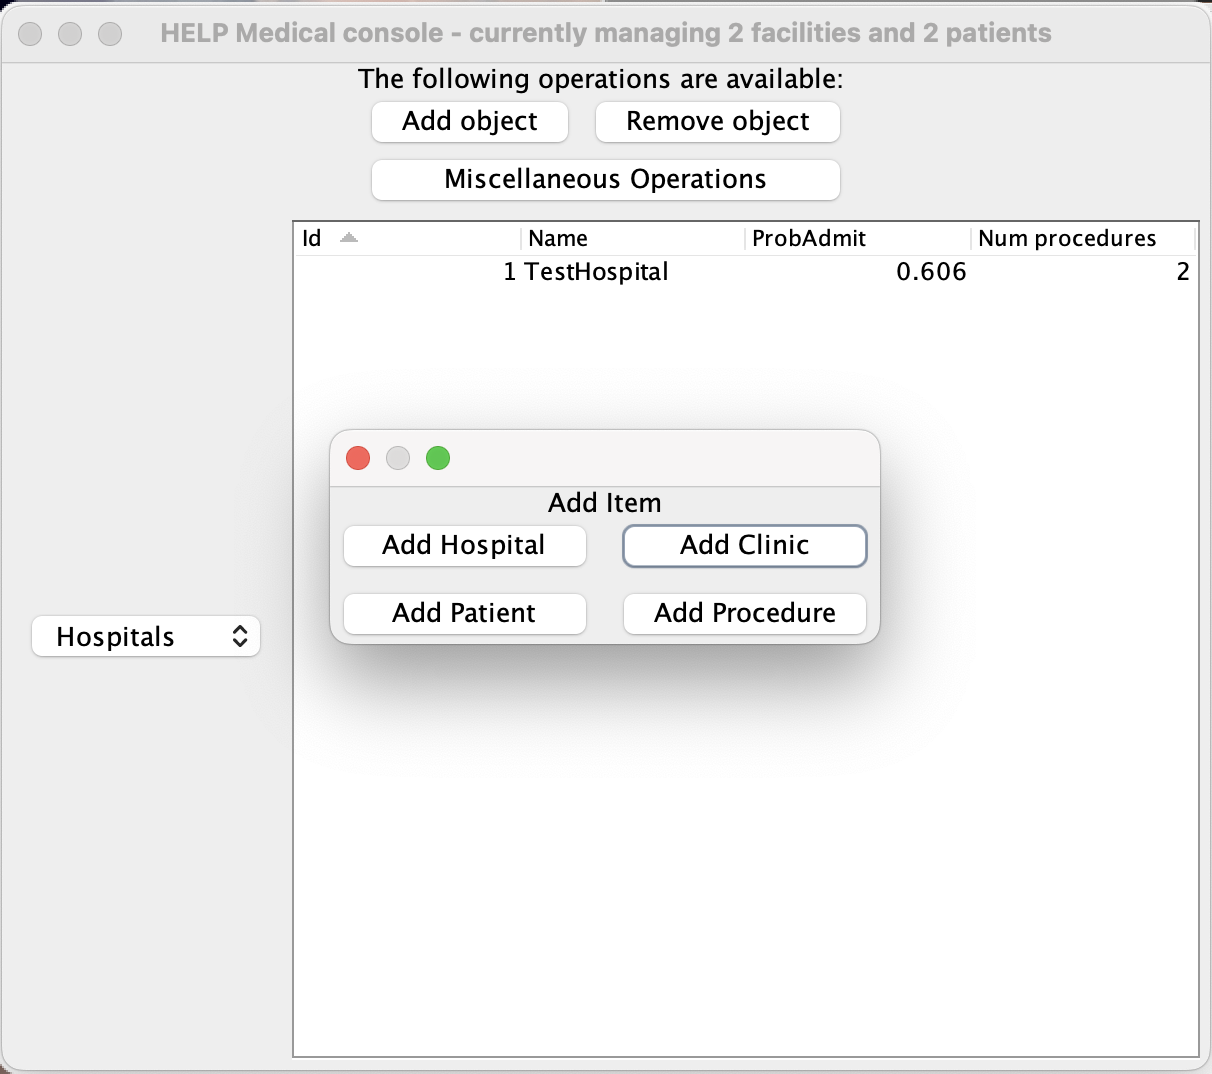
\includegraphics[width=0.5\textwidth]{./figures/Add/Clinic_1.png}
  \end{center}
\end{figure}

\begin{figure}
  \begin{center}
    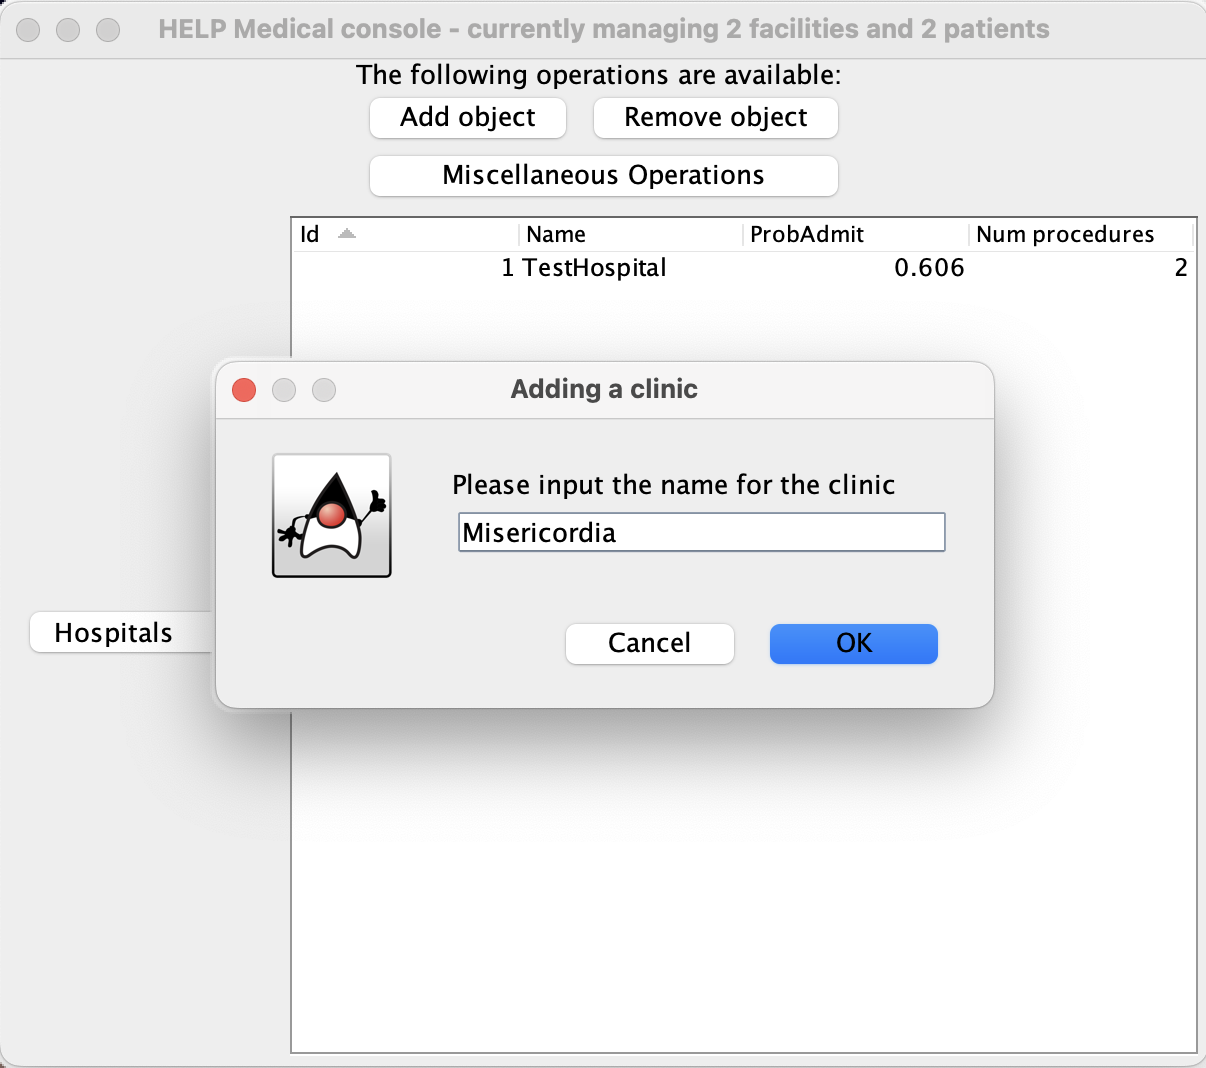
\includegraphics[width=0.5\textwidth]{./figures/Add/Clinic_2.png}
  \end{center}
\end{figure}

\begin{figure}
  \begin{center}
    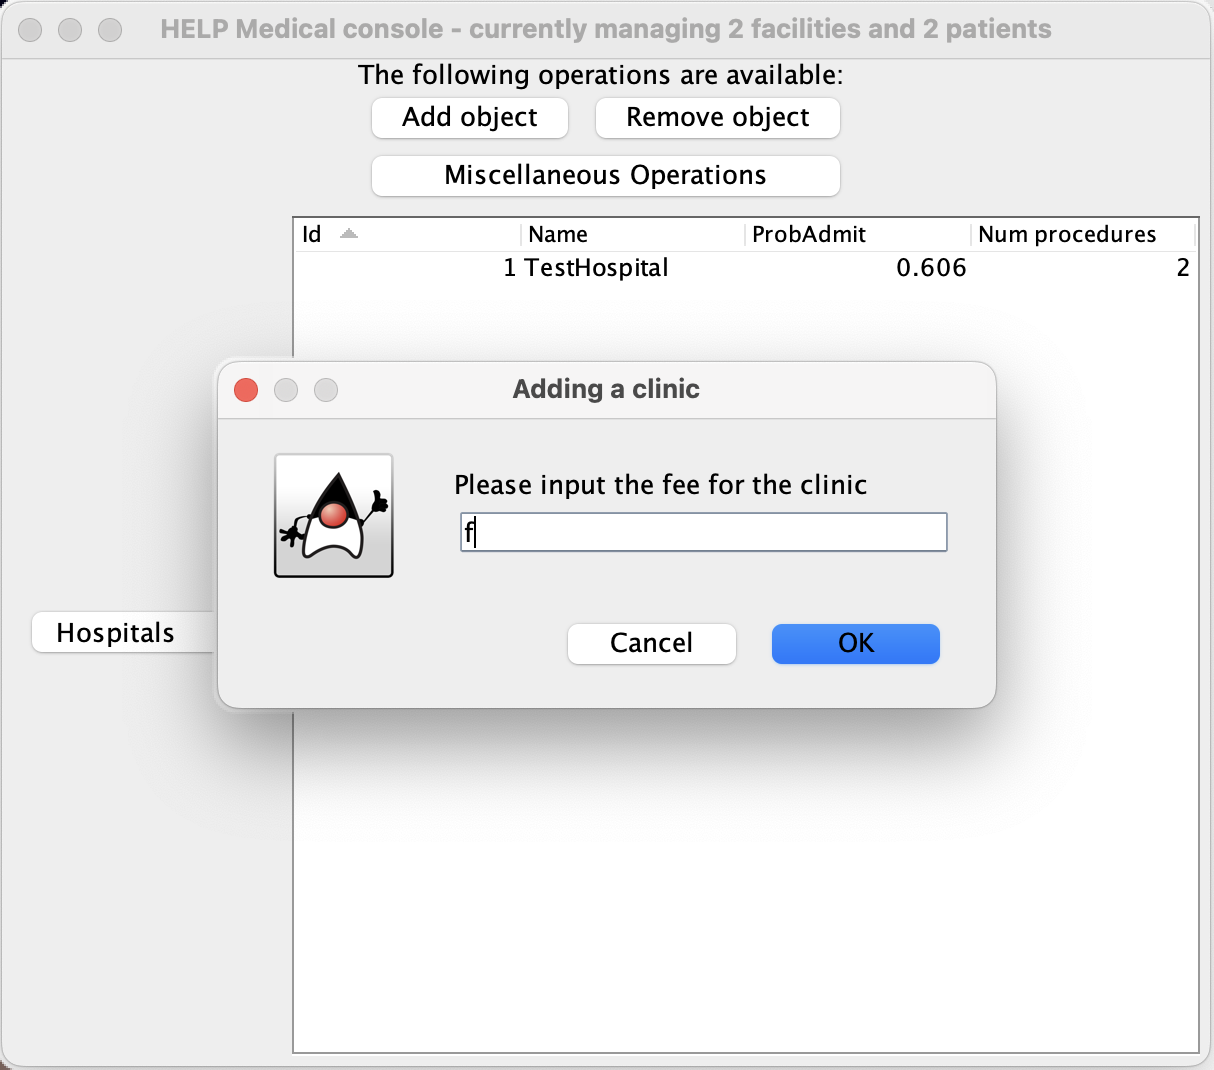
\includegraphics[width=0.5\textwidth]{./figures/Add/Clinic_3.png}
  \end{center}
\end{figure}

As can be seen from the picture above, the application prevents invalid inputs by the user. Furthermore, the user can also cancel their inputs anytime during the input process. This validation is true for all that can be input.

\begin{figure}
  \begin{center}
    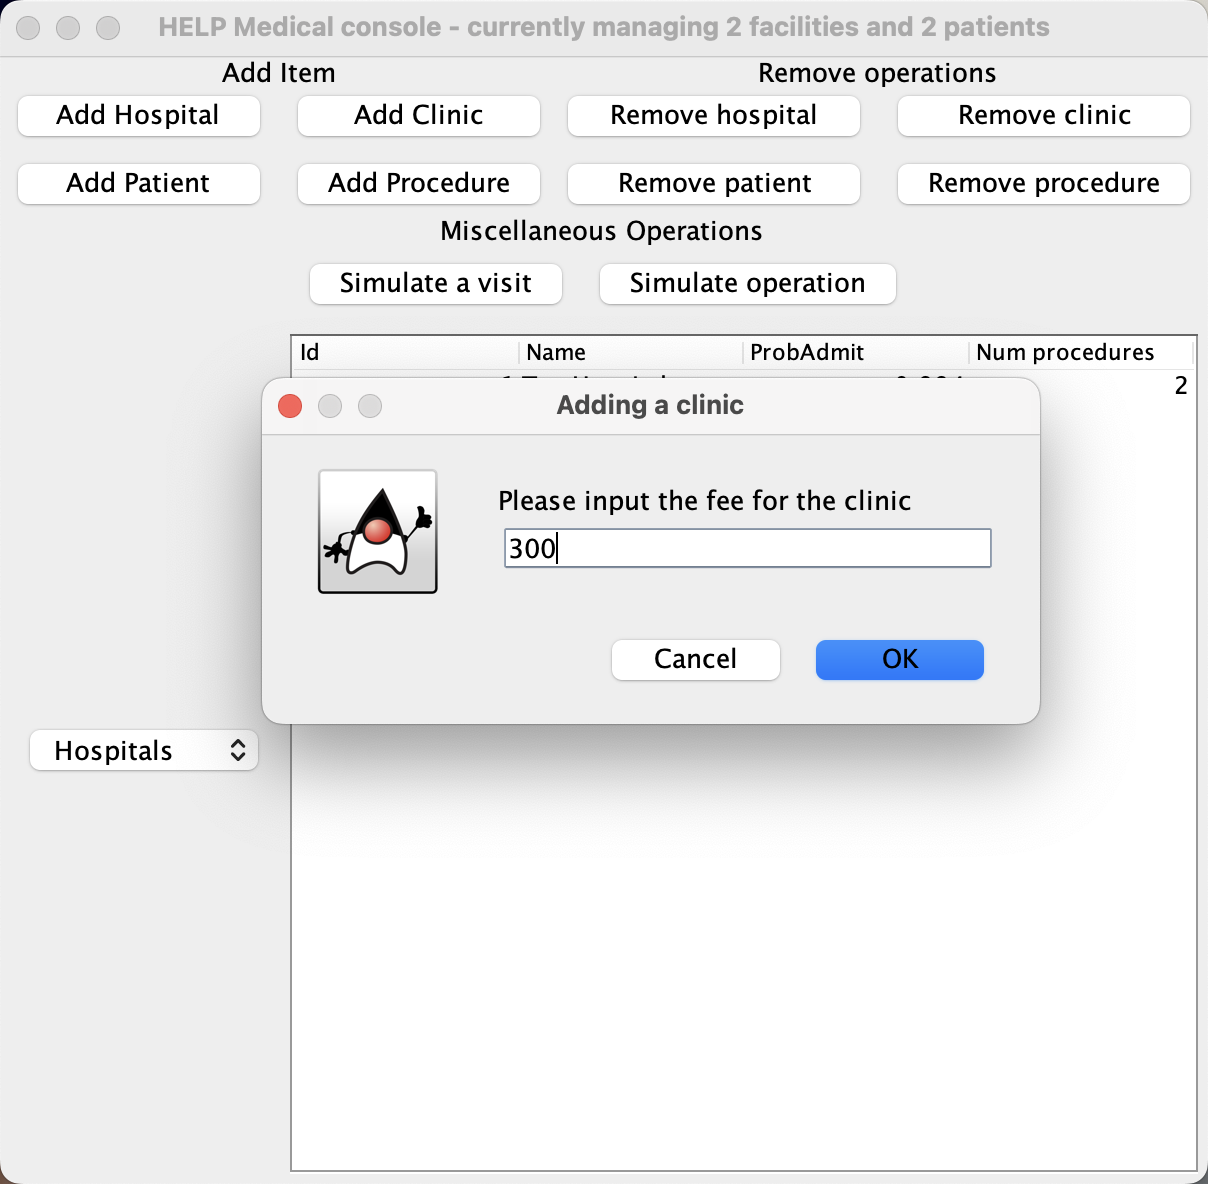
\includegraphics[width=0.5\textwidth]{./figures/Add/Clinic_4.png}
  \end{center}
\end{figure}

\begin{figure}
  \begin{center}
    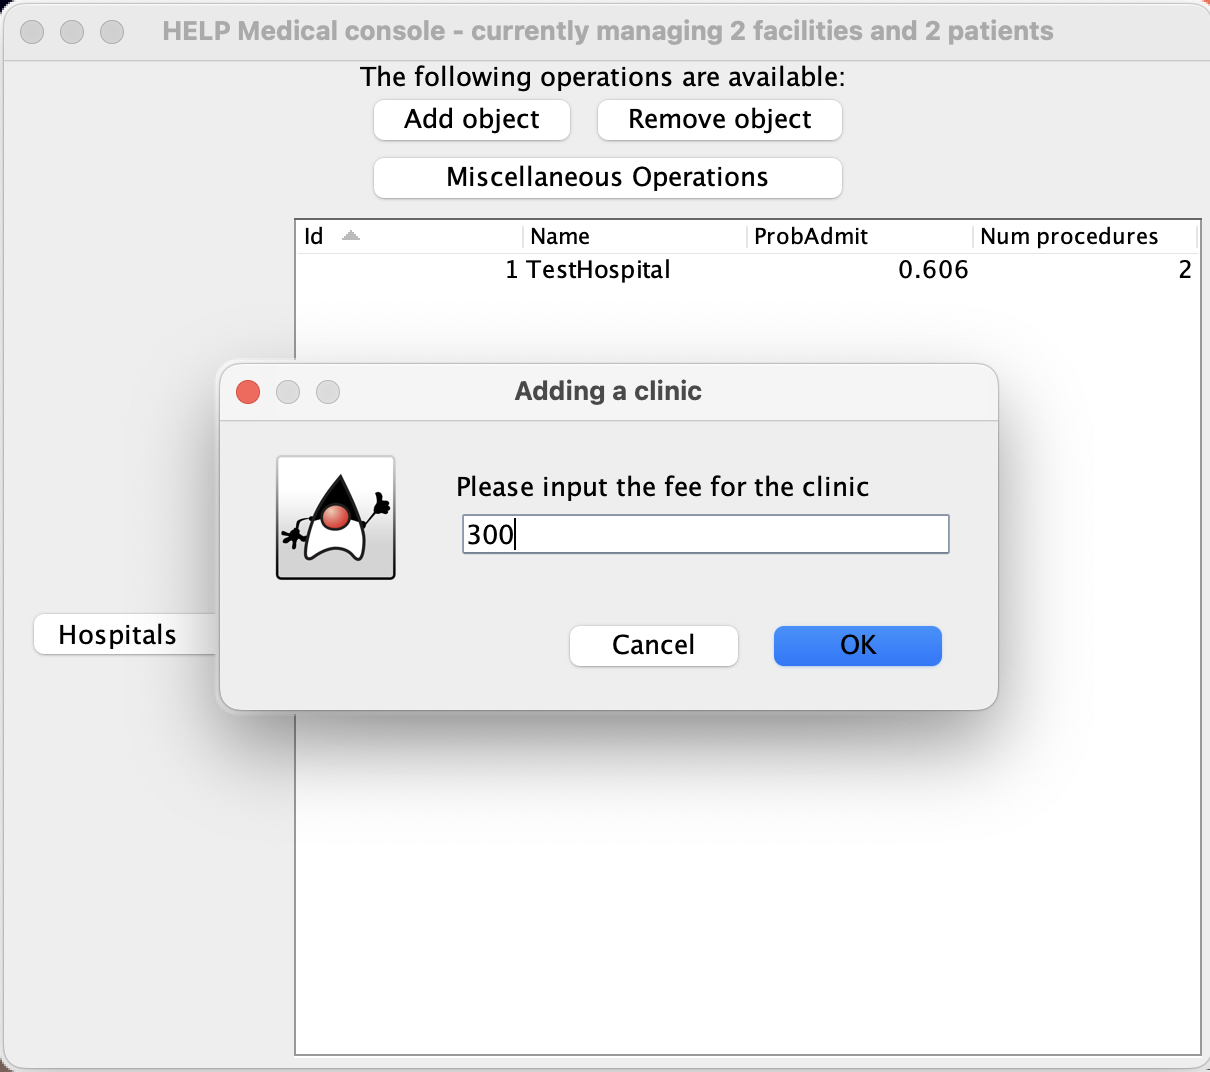
\includegraphics[width=0.5\textwidth]{./figures/Add/Clinic_5.png}
  \end{center}
\end{figure}

\begin{figure}
  \begin{center}
    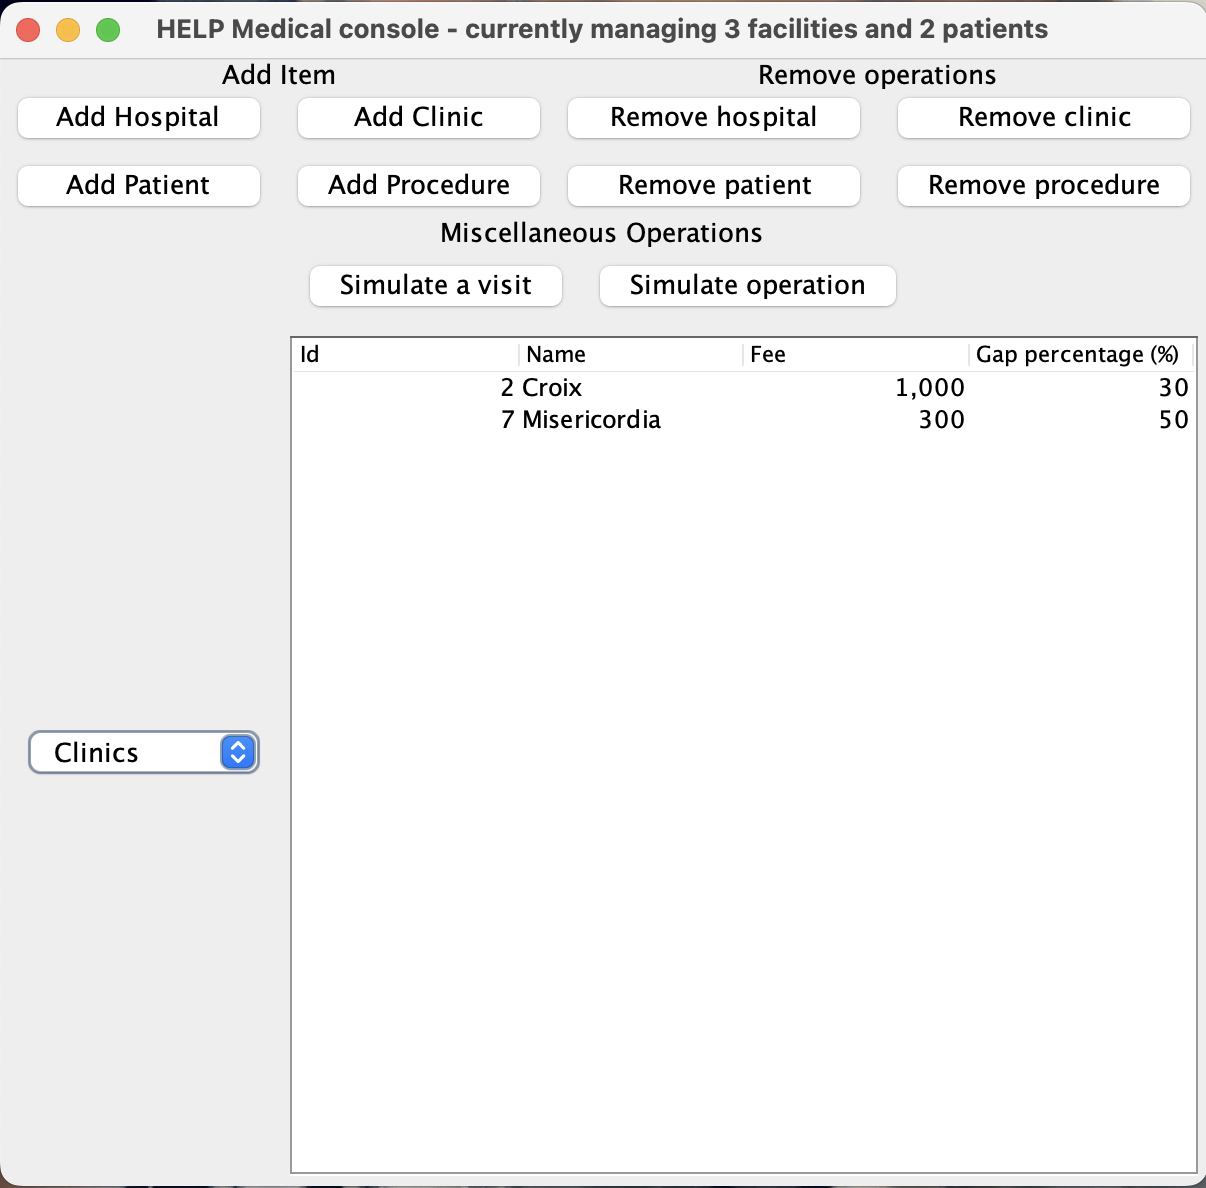
\includegraphics[width=0.5\textwidth]{./figures/Add/Clinic_6.png}
  \end{center}
\end{figure}

\begin{figure}
  \begin{center}
    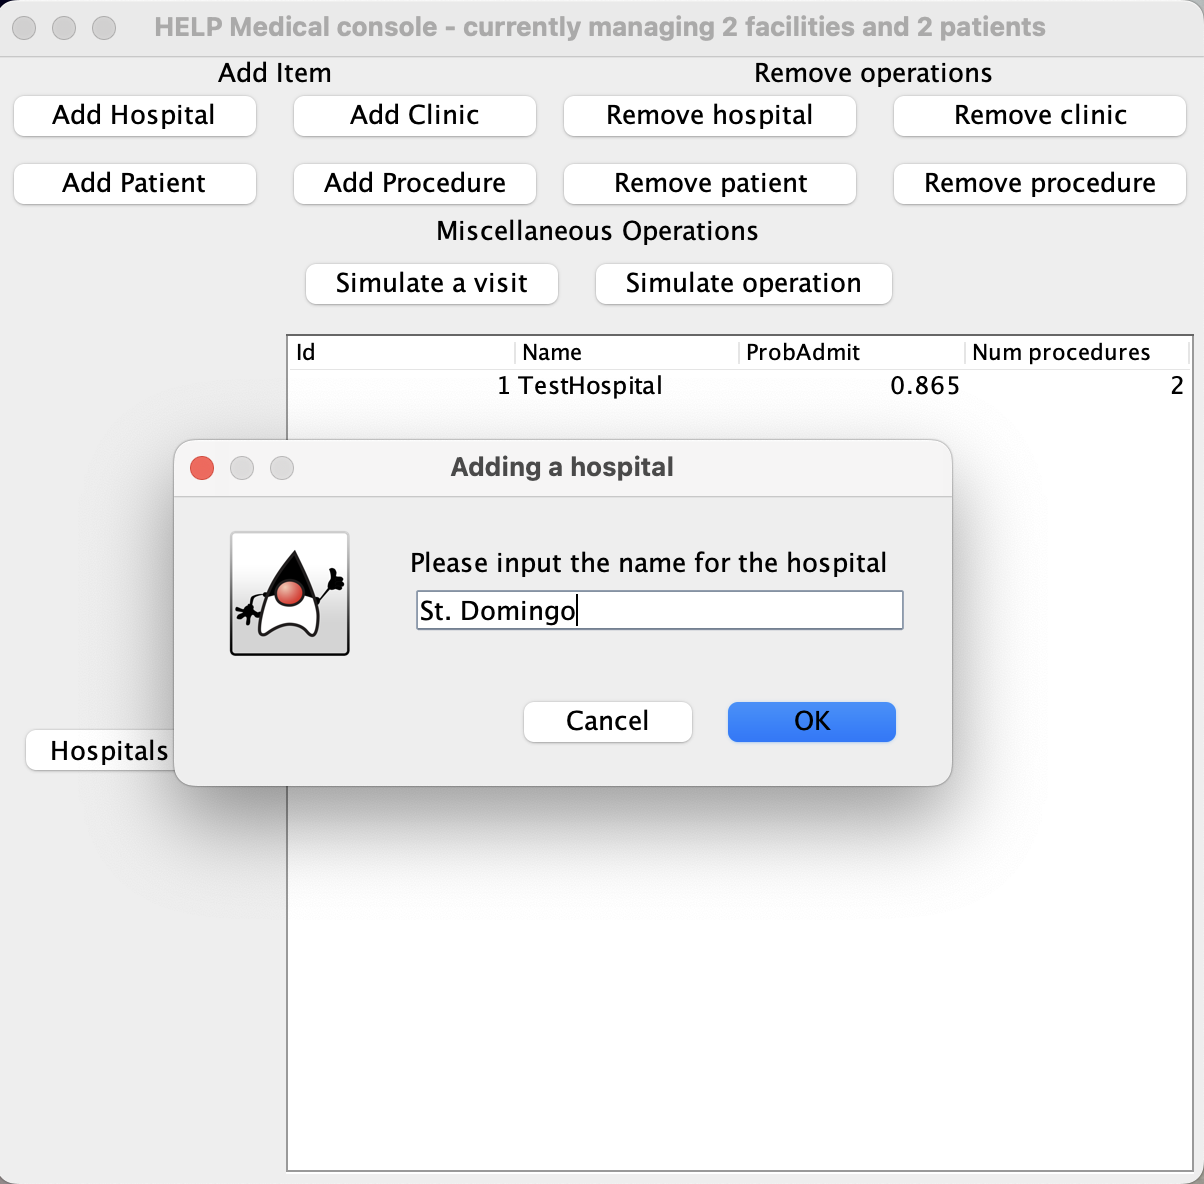
\includegraphics[width=0.5\textwidth]{./figures/Add/Hospital_1.png}
  \end{center}
\end{figure}

\begin{figure}
  \begin{center}
    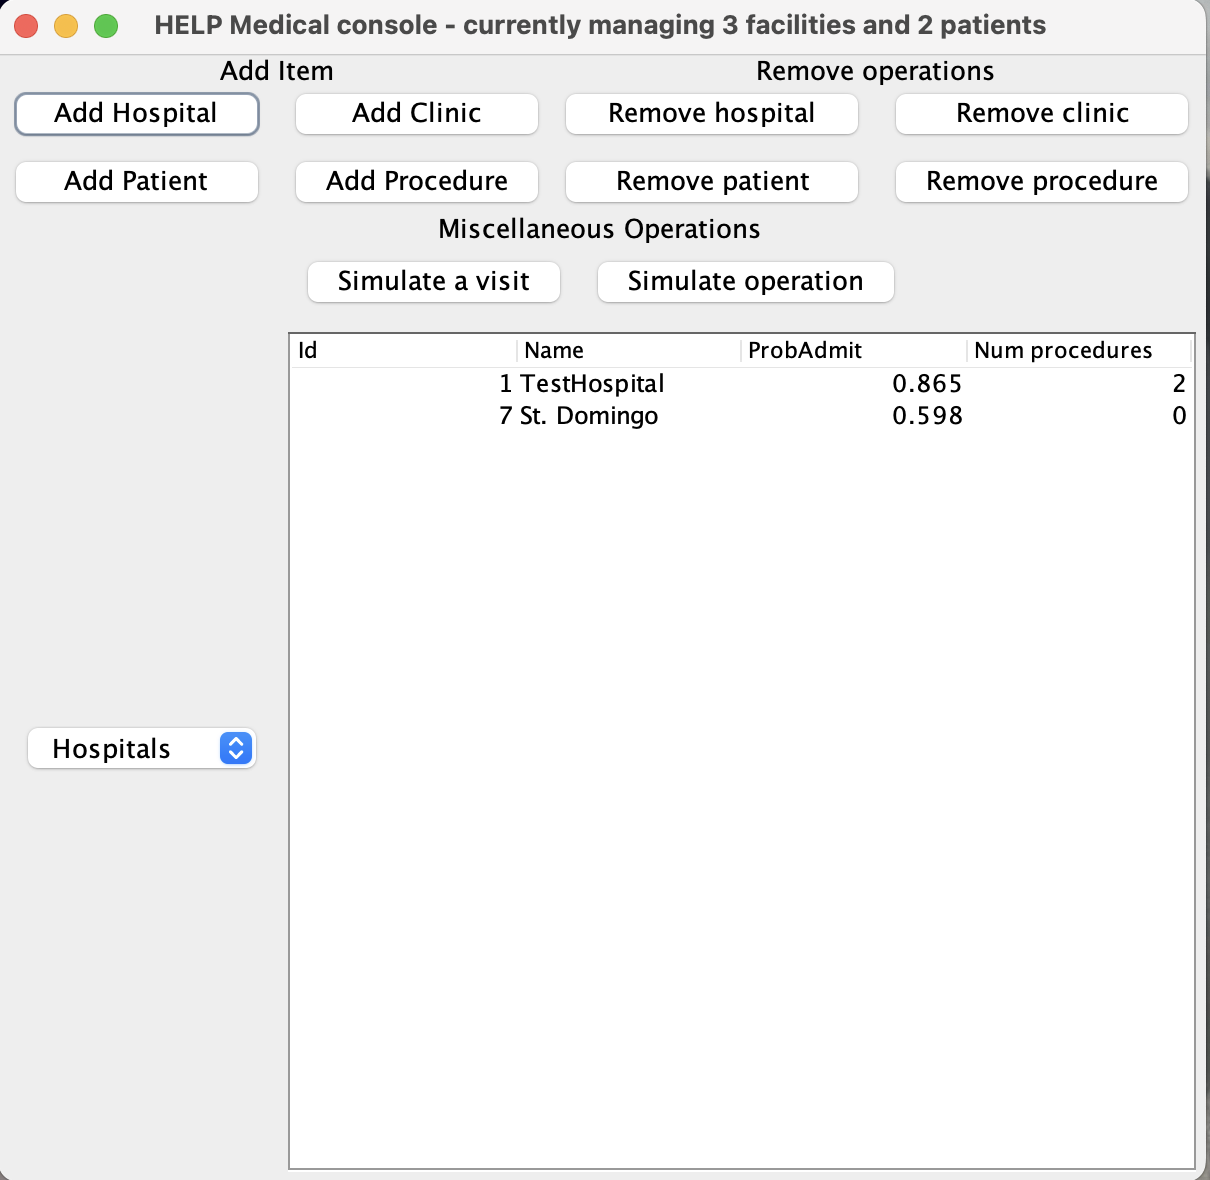
\includegraphics[width=0.5\textwidth]{./figures/Add/Hospital_2.png}
  \end{center}
\end{figure}

\begin{figure}
  \begin{center}
    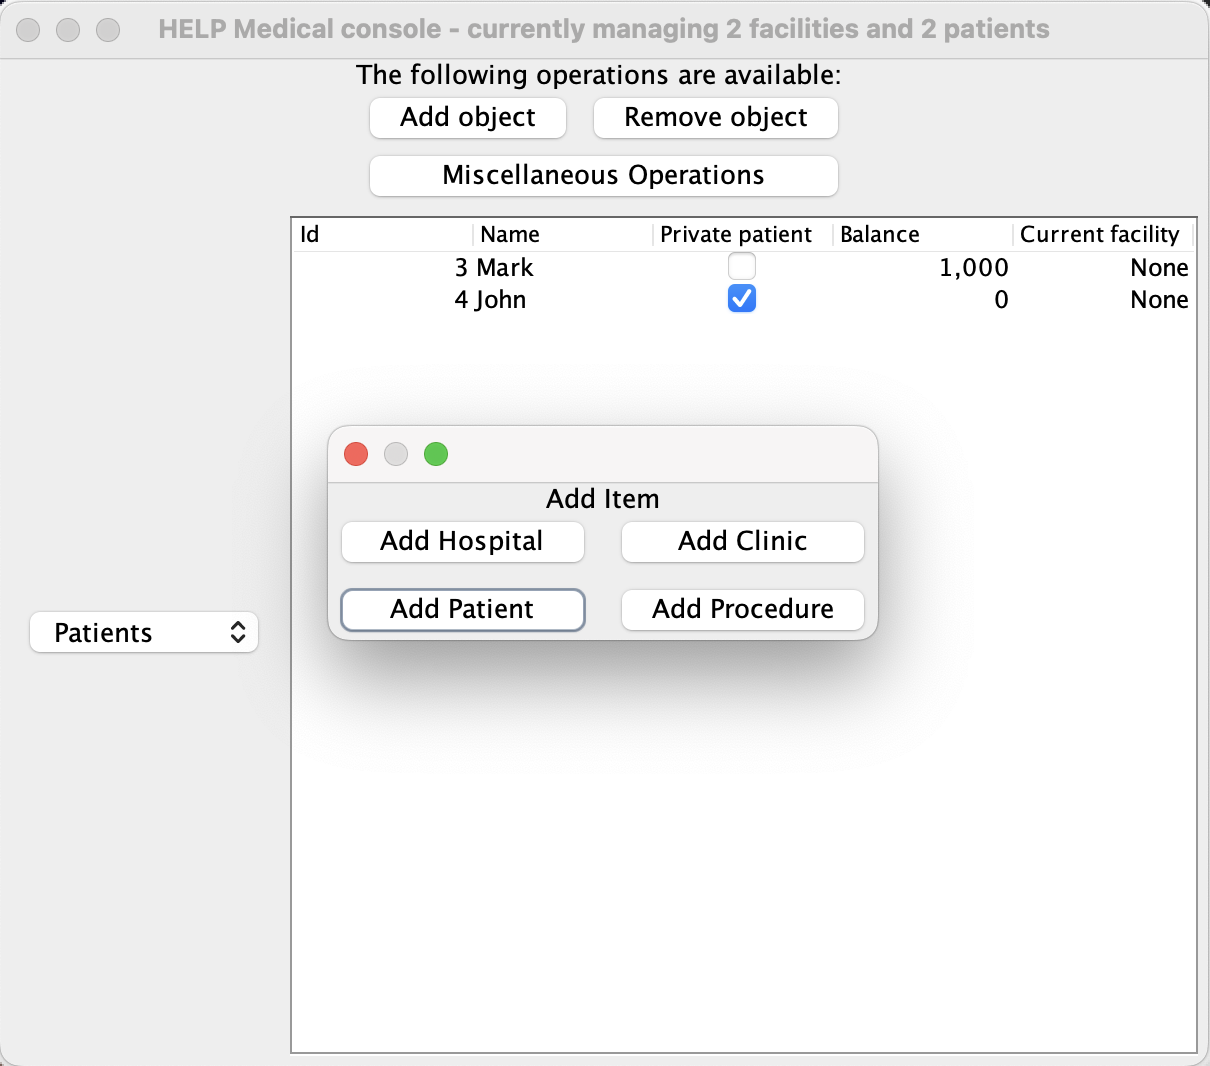
\includegraphics[width=0.5\textwidth]{./figures/Add/Patient_1.png}
  \end{center}
\end{figure}

\begin{figure}
  \begin{center}
    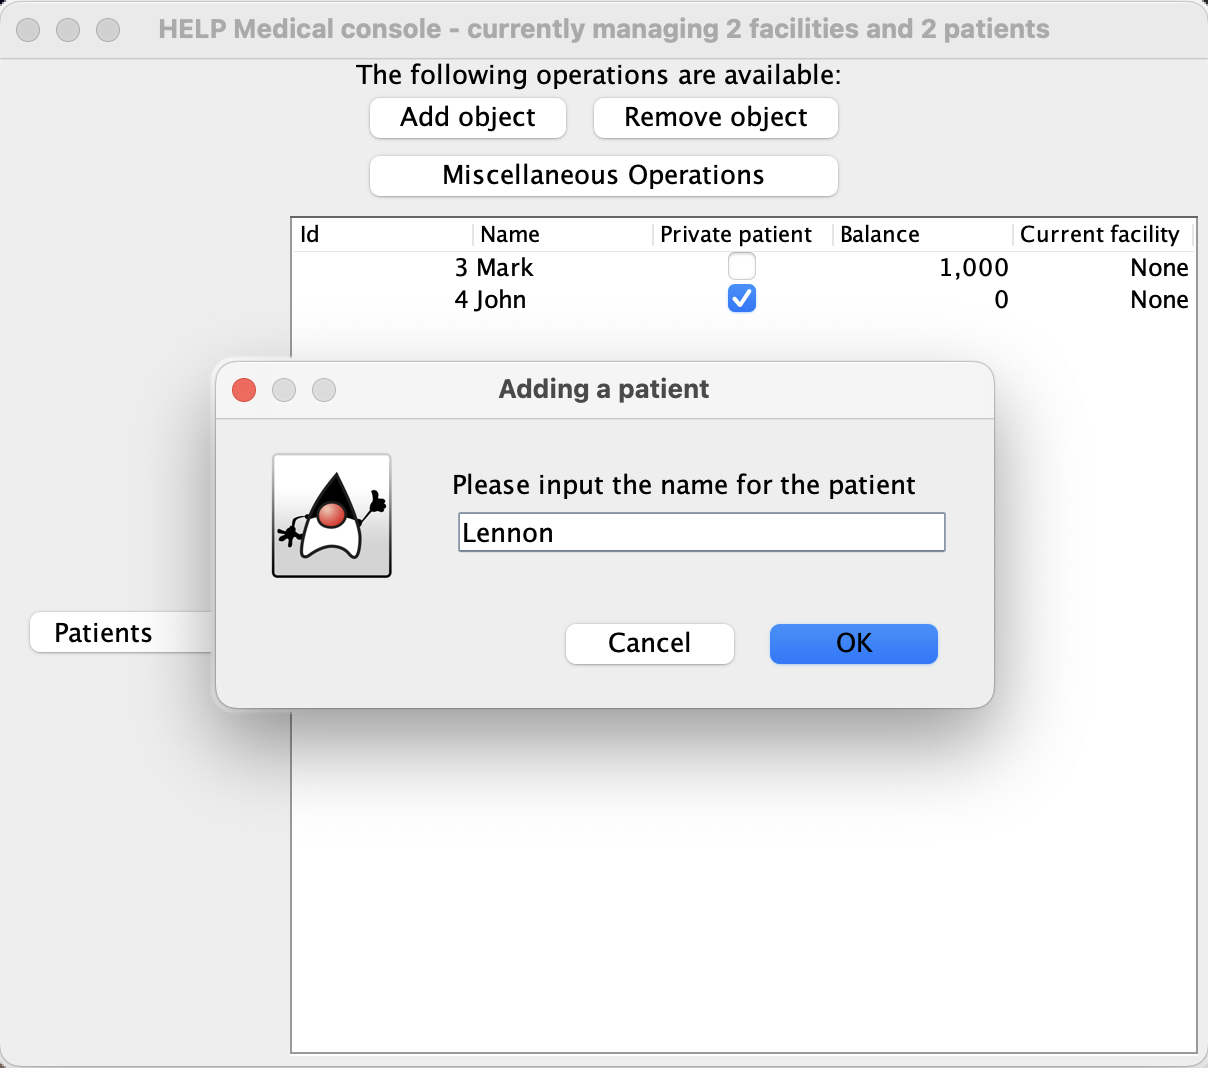
\includegraphics[width=0.5\textwidth]{./figures/Add/Patient_2.png}
  \end{center}
\end{figure}

\begin{figure}
  \begin{center}
    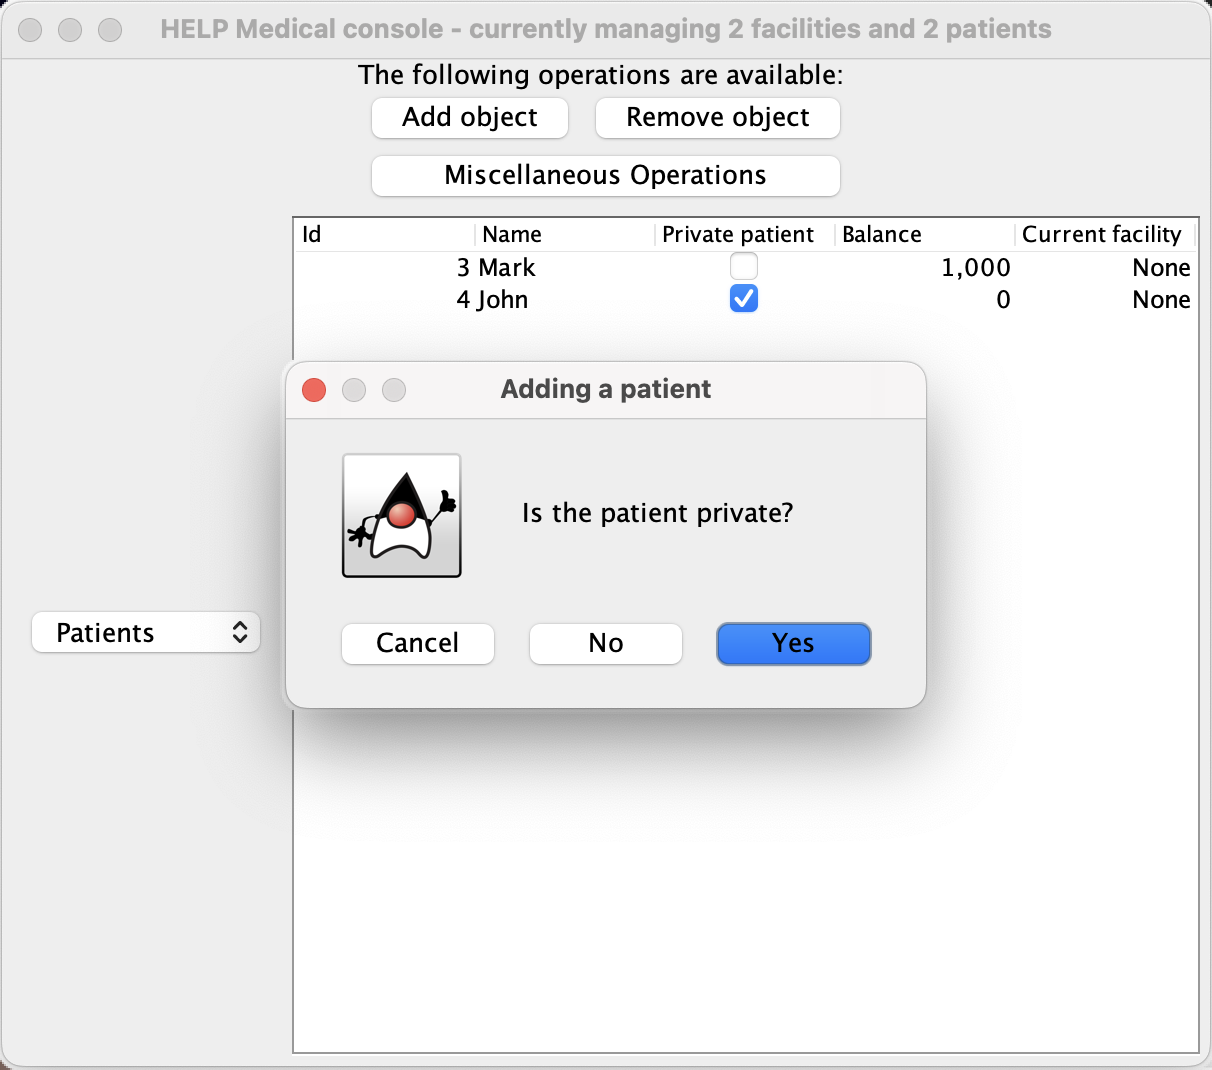
\includegraphics[width=0.5\textwidth]{./figures/Add/Patient_3.png}
  \end{center}
\end{figure}

\begin{figure}
  \begin{center}
    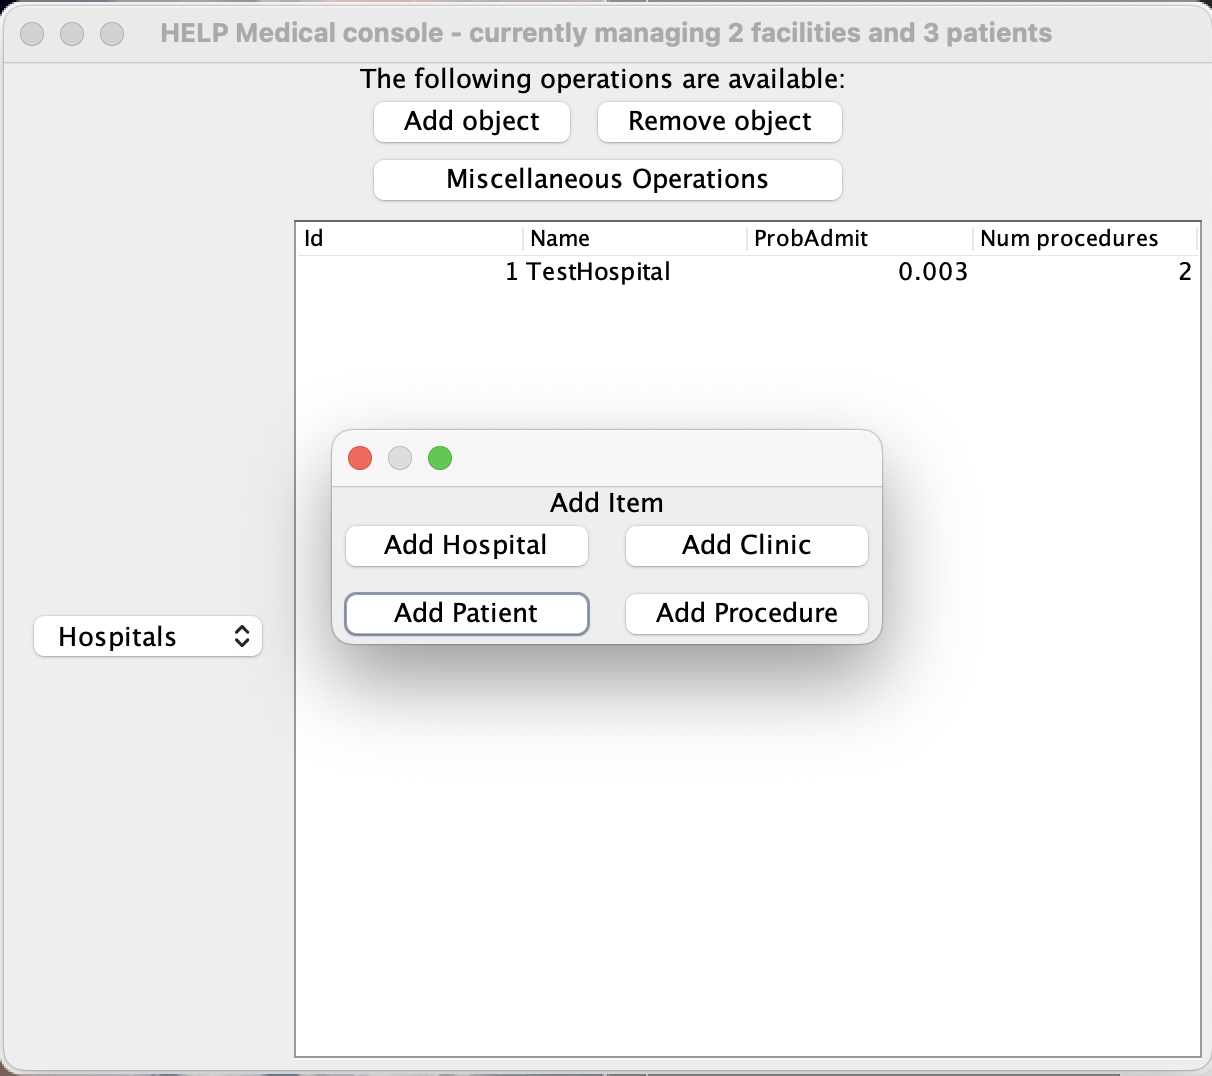
\includegraphics[width=0.5\textwidth]{./figures/Add/Procedure_1.png}
  \end{center}
\end{figure}

\begin{figure}
  \begin{center}
    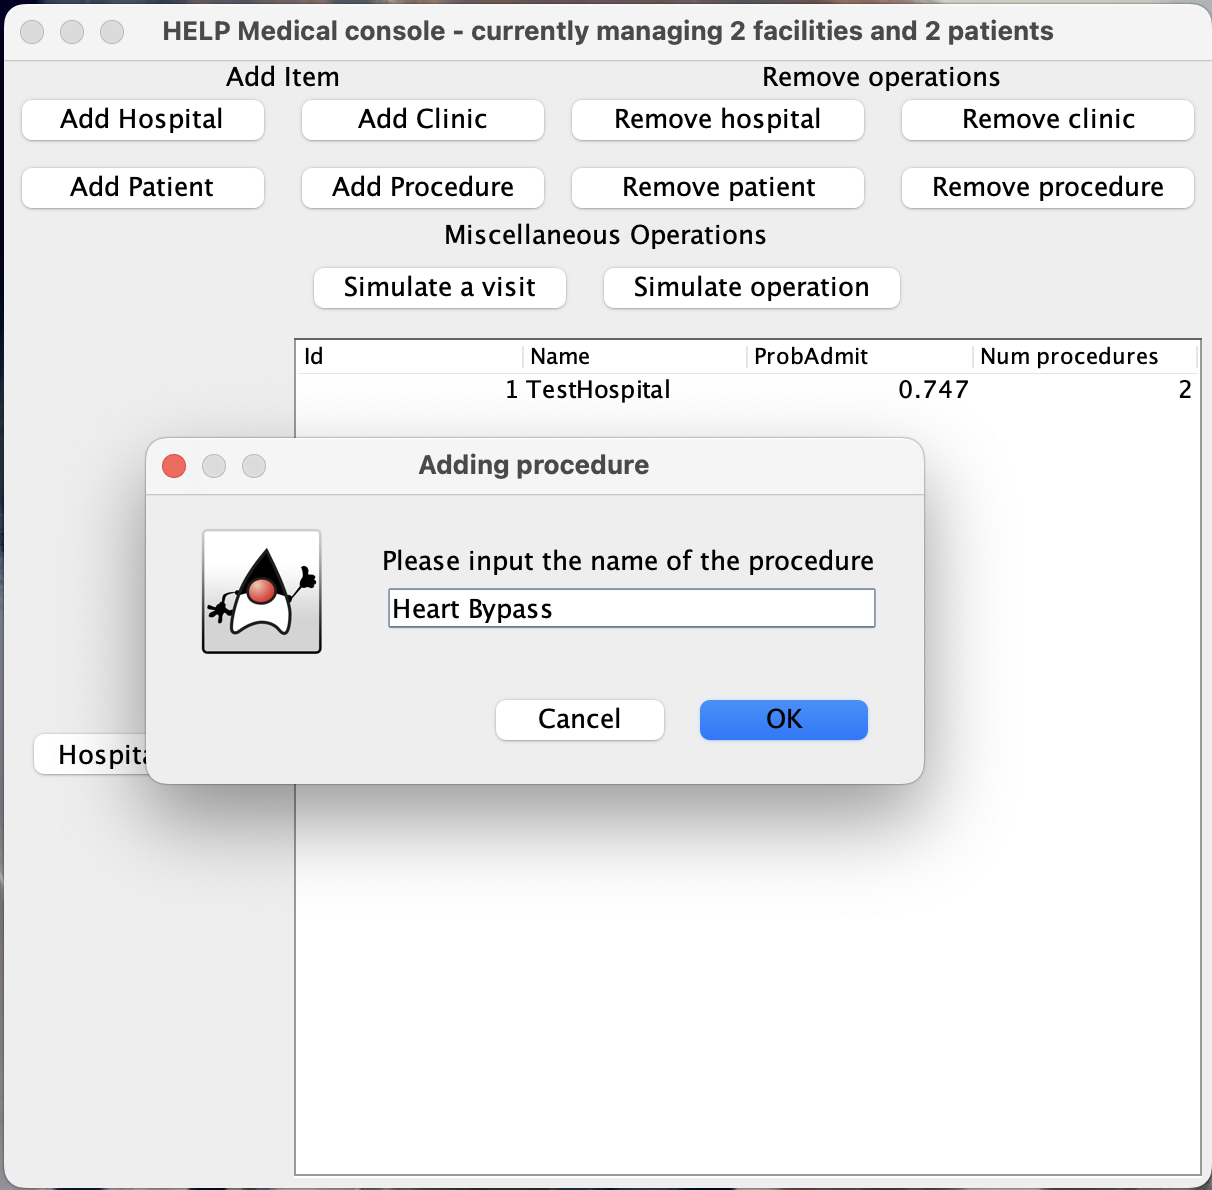
\includegraphics[width=0.5\textwidth]{./figures/Add/Procedure_2.png}
  \end{center}
\end{figure}

\begin{figure}
  \begin{center}
    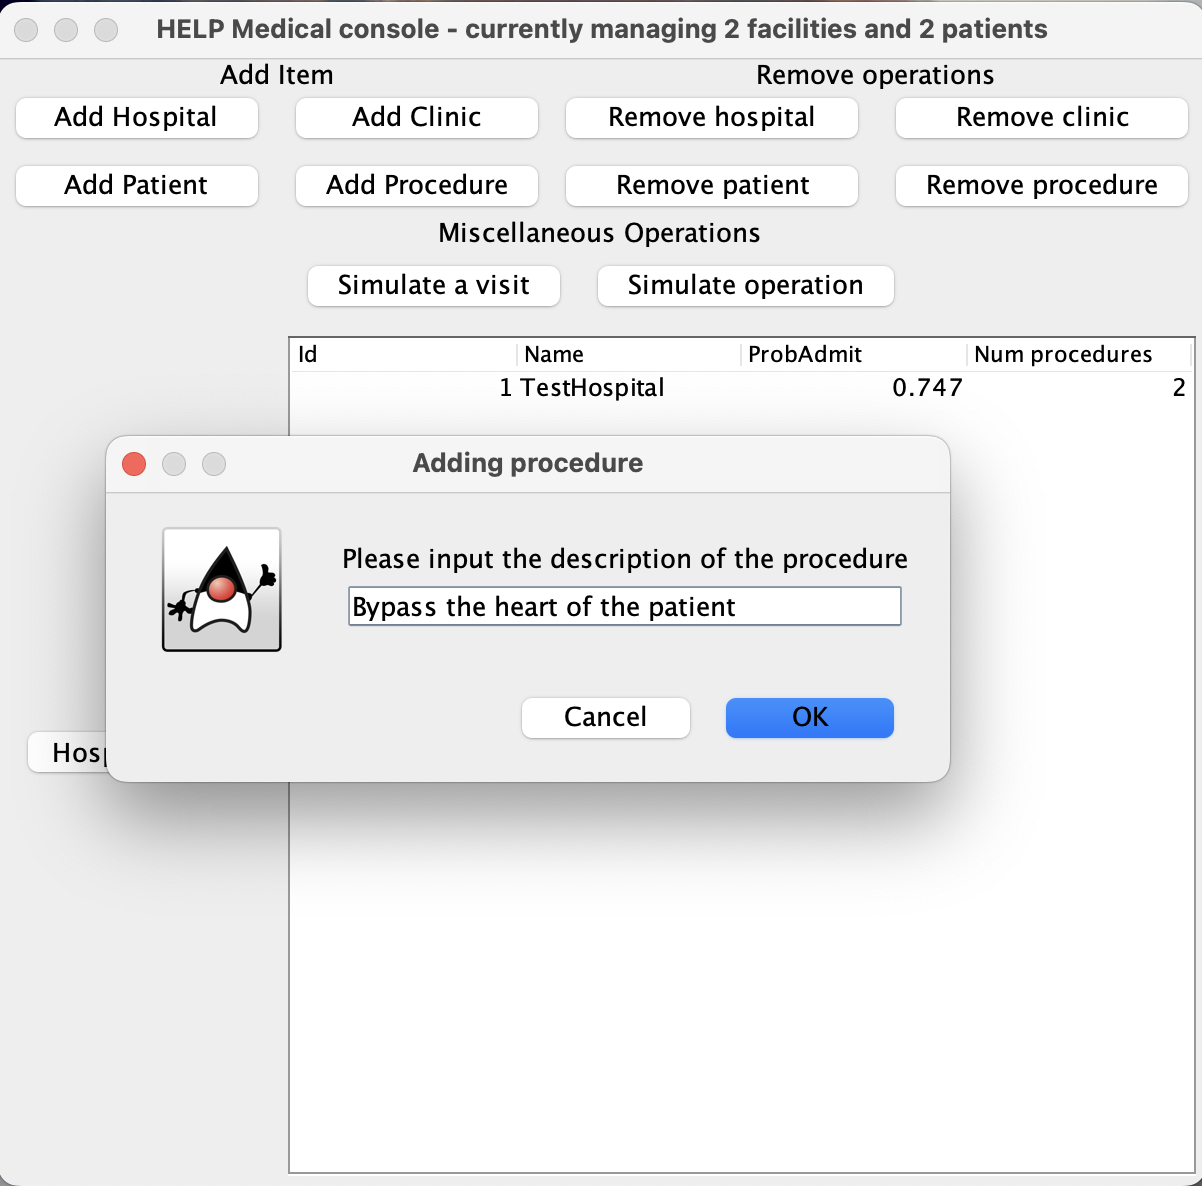
\includegraphics[width=0.5\textwidth]{./figures/Add/Procedure_3.png}
  \end{center}
\end{figure}

\begin{figure}
  \begin{center}
    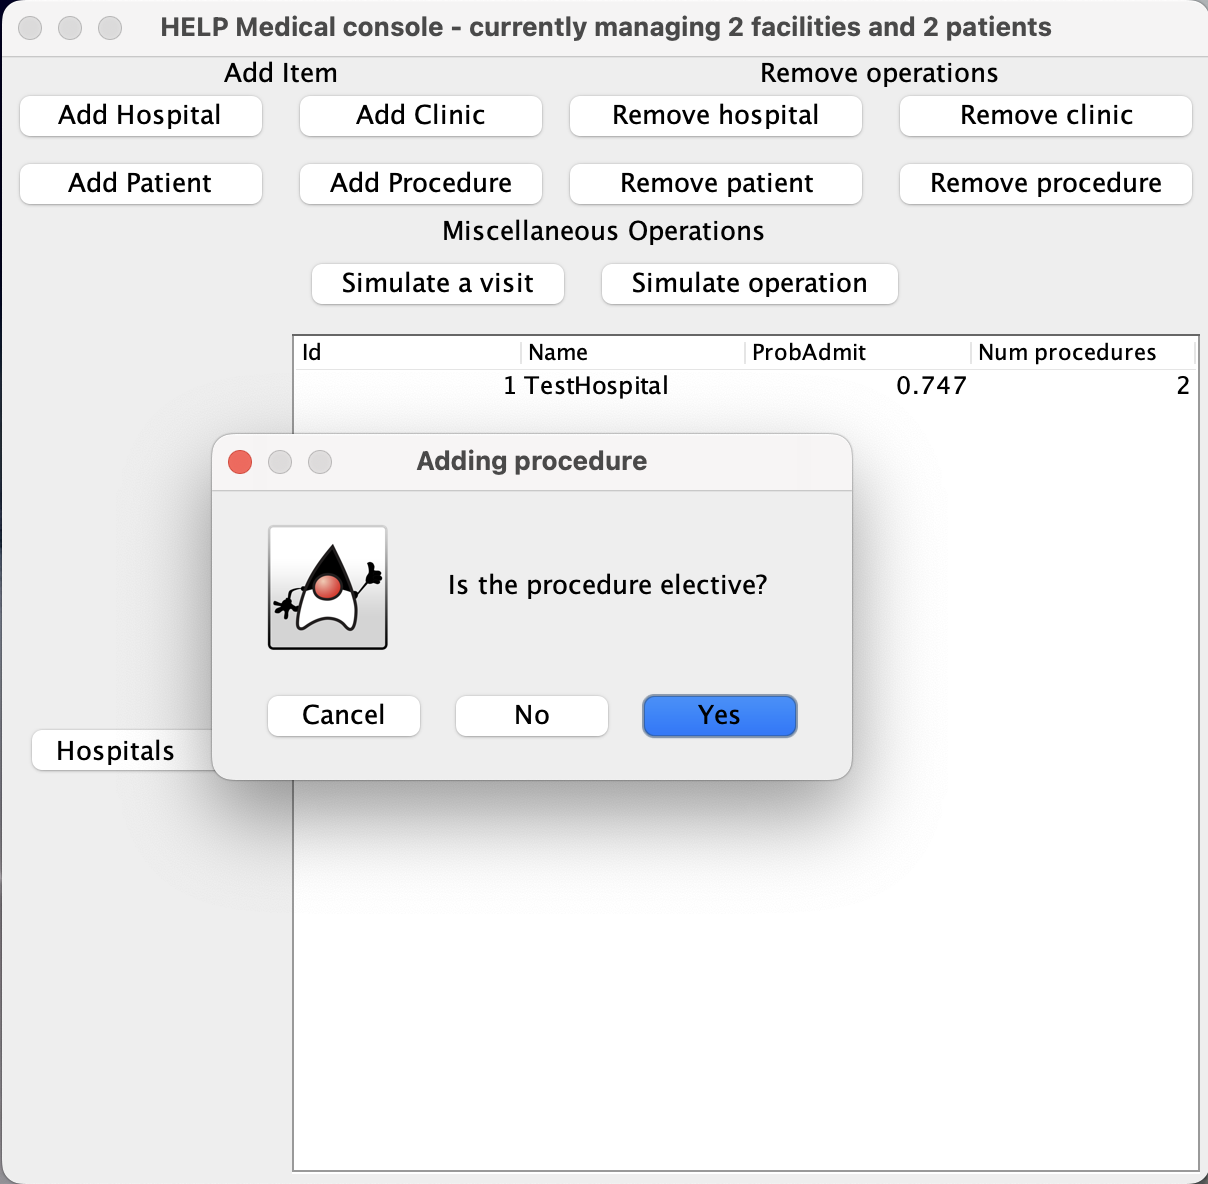
\includegraphics[width=0.5\textwidth]{./figures/Add/Procedure_4.png}
  \end{center}
\end{figure}

\begin{figure}
  \begin{center}
    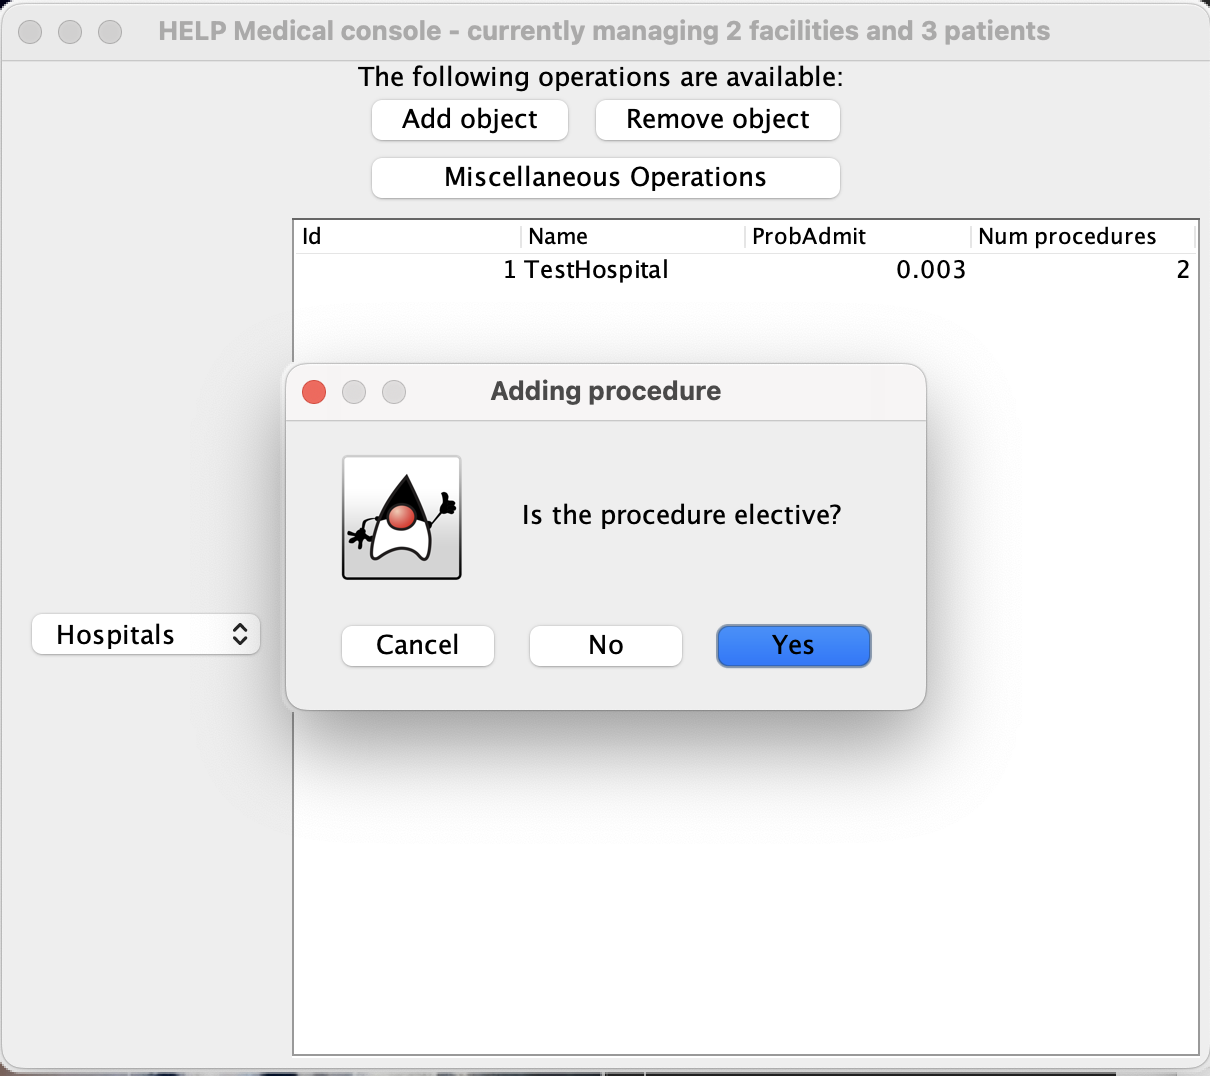
\includegraphics[width=0.5\textwidth]{./figures/Add/Procedure_5.png}
  \end{center}
\end{figure}

\begin{figure}
  \begin{center}
    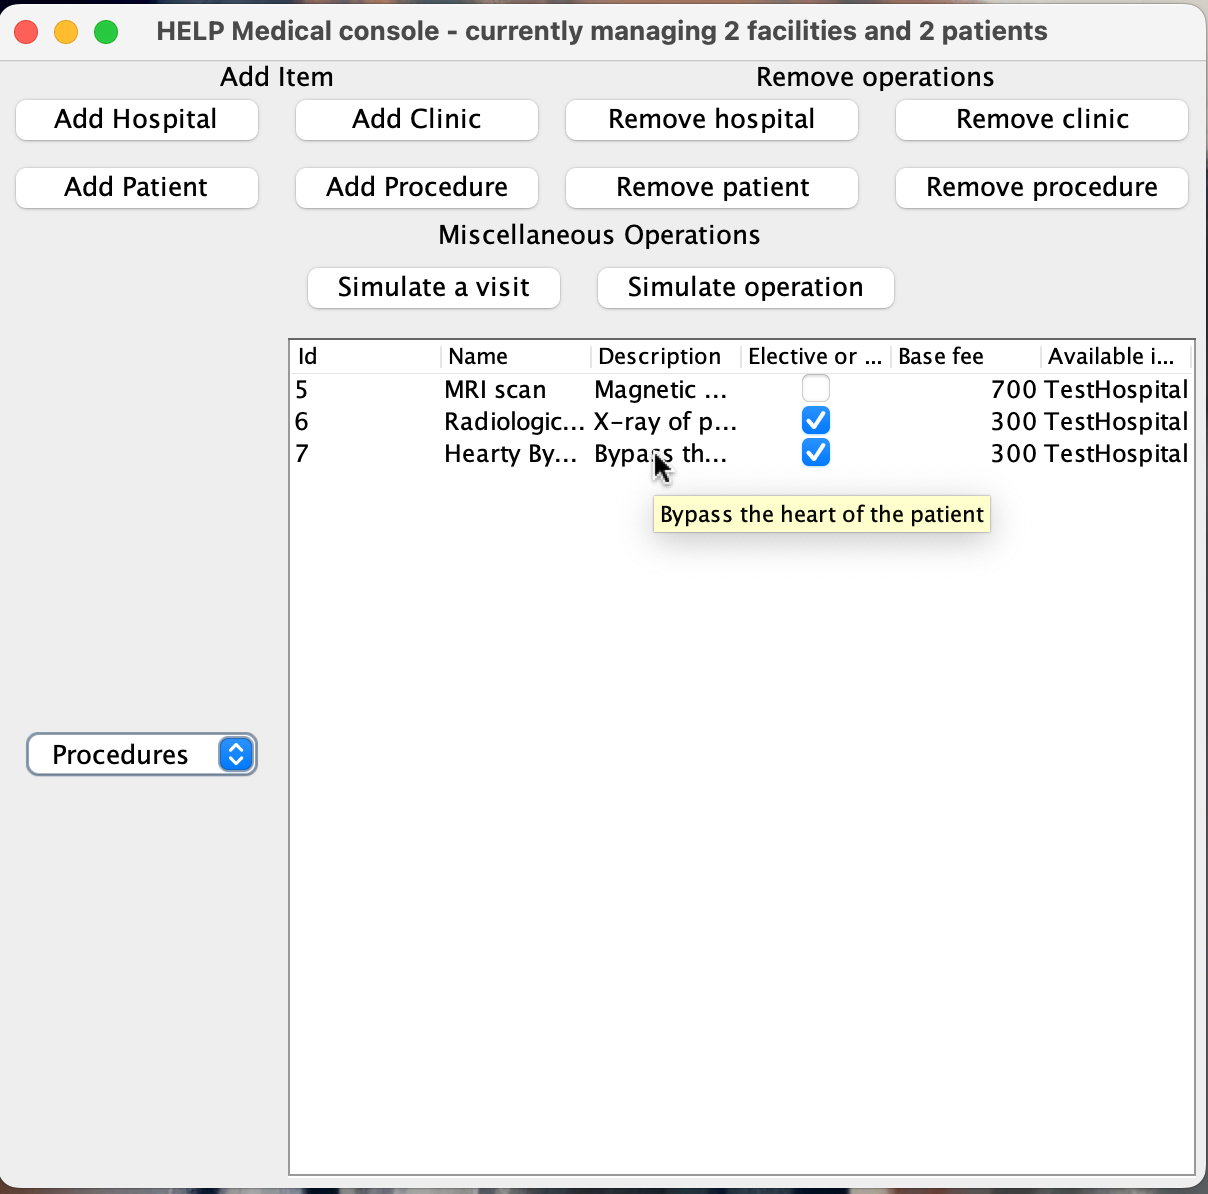
\includegraphics[width=0.8\textwidth]{./figures/Add/Procedure_6.png}
  \end{center}
\end{figure}
% subsection Adding (end)

\subsection{Removing}\label{sub:removing}
\begin{figure}
  \begin{center}
  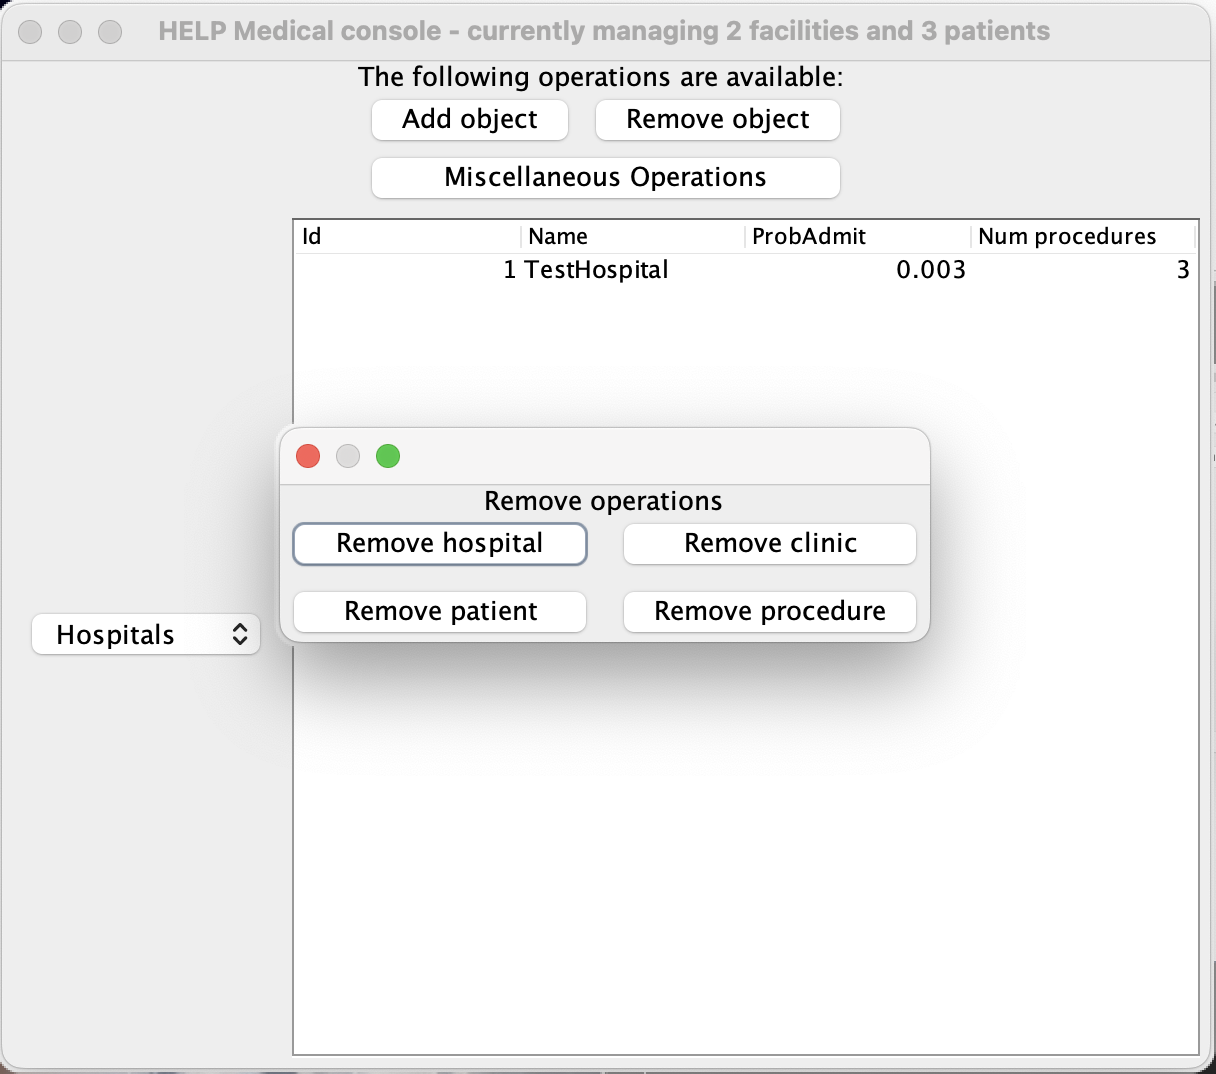
\includegraphics[width=0.5\textwidth]{./figures/Remove/Hospital_1.png}
  \end{center}
\end{figure}

\begin{figure}
  \begin{center}
  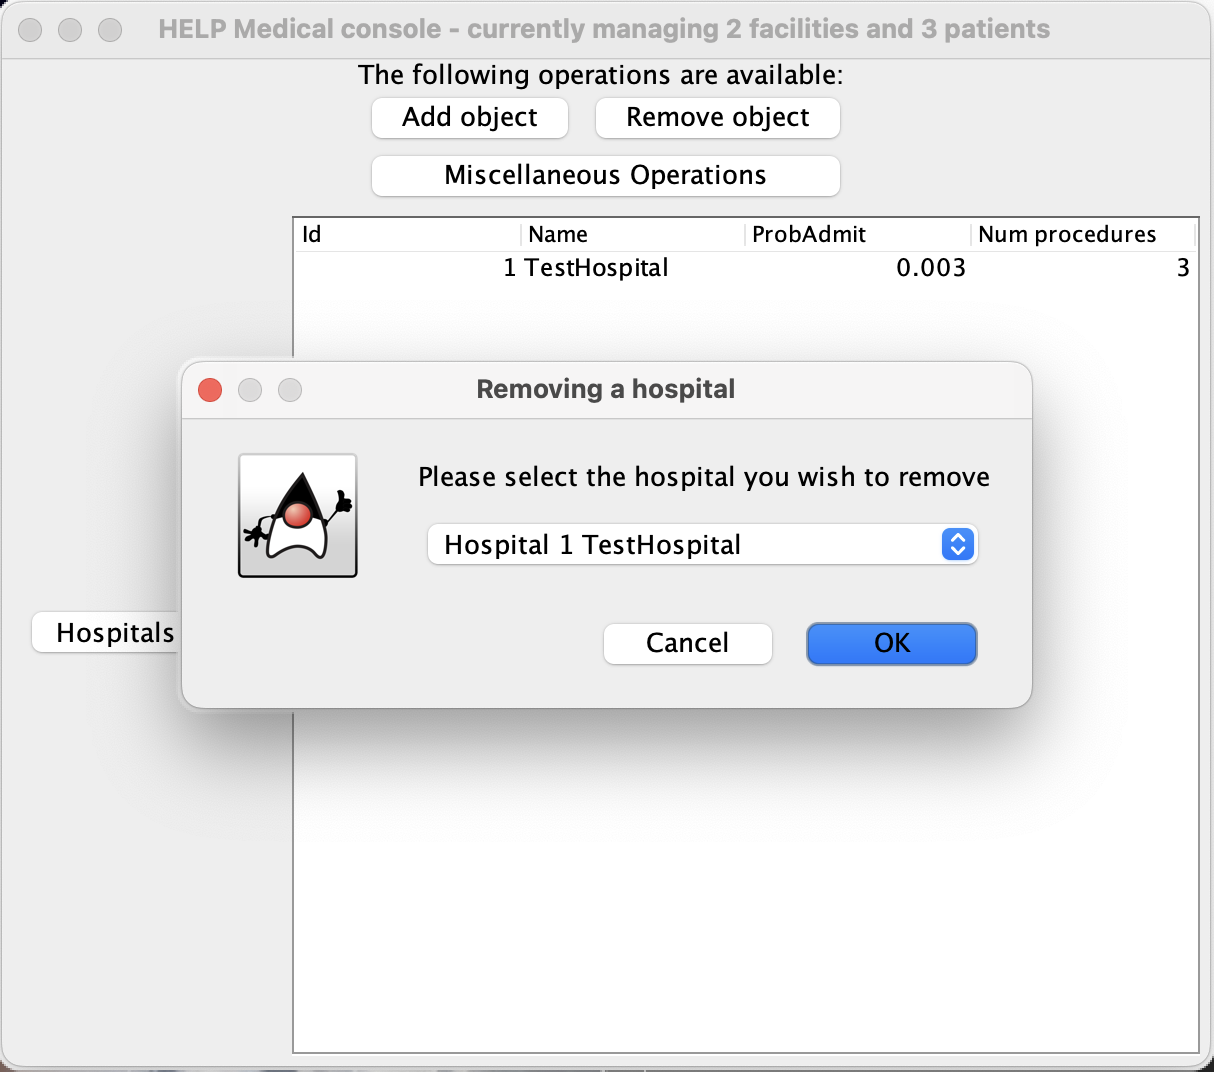
\includegraphics[width=0.5\textwidth]{./figures/Remove/Hospital_2.png}
  \end{center}
\end{figure}

\begin{figure}
  \begin{center}
  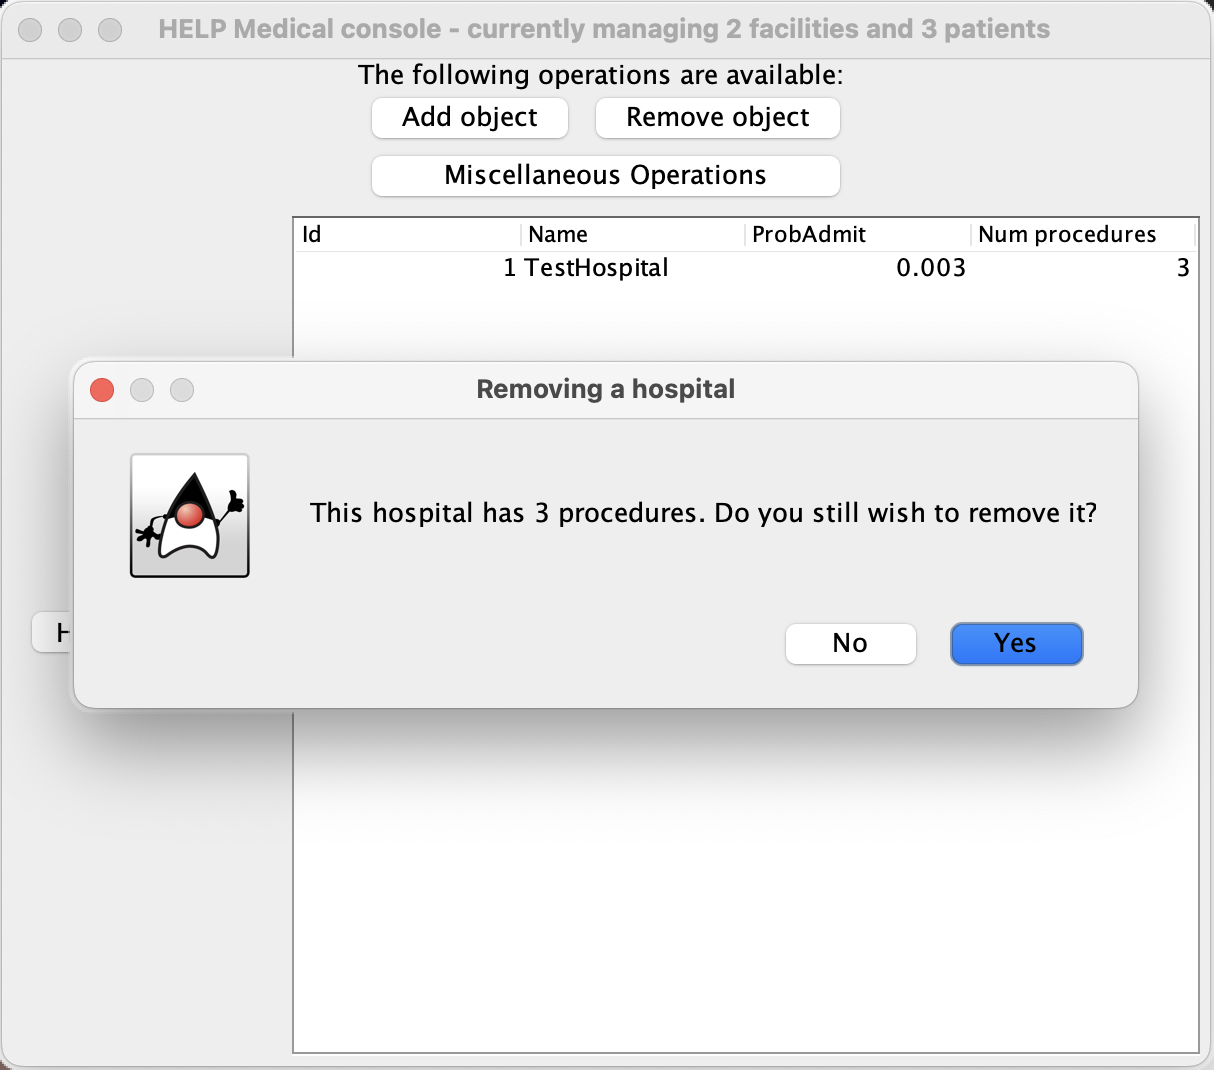
\includegraphics[width=0.5\textwidth]{./figures/Remove/Hospital_3.png}
  \end{center}
\end{figure}

\begin{figure}
  \begin{center}
  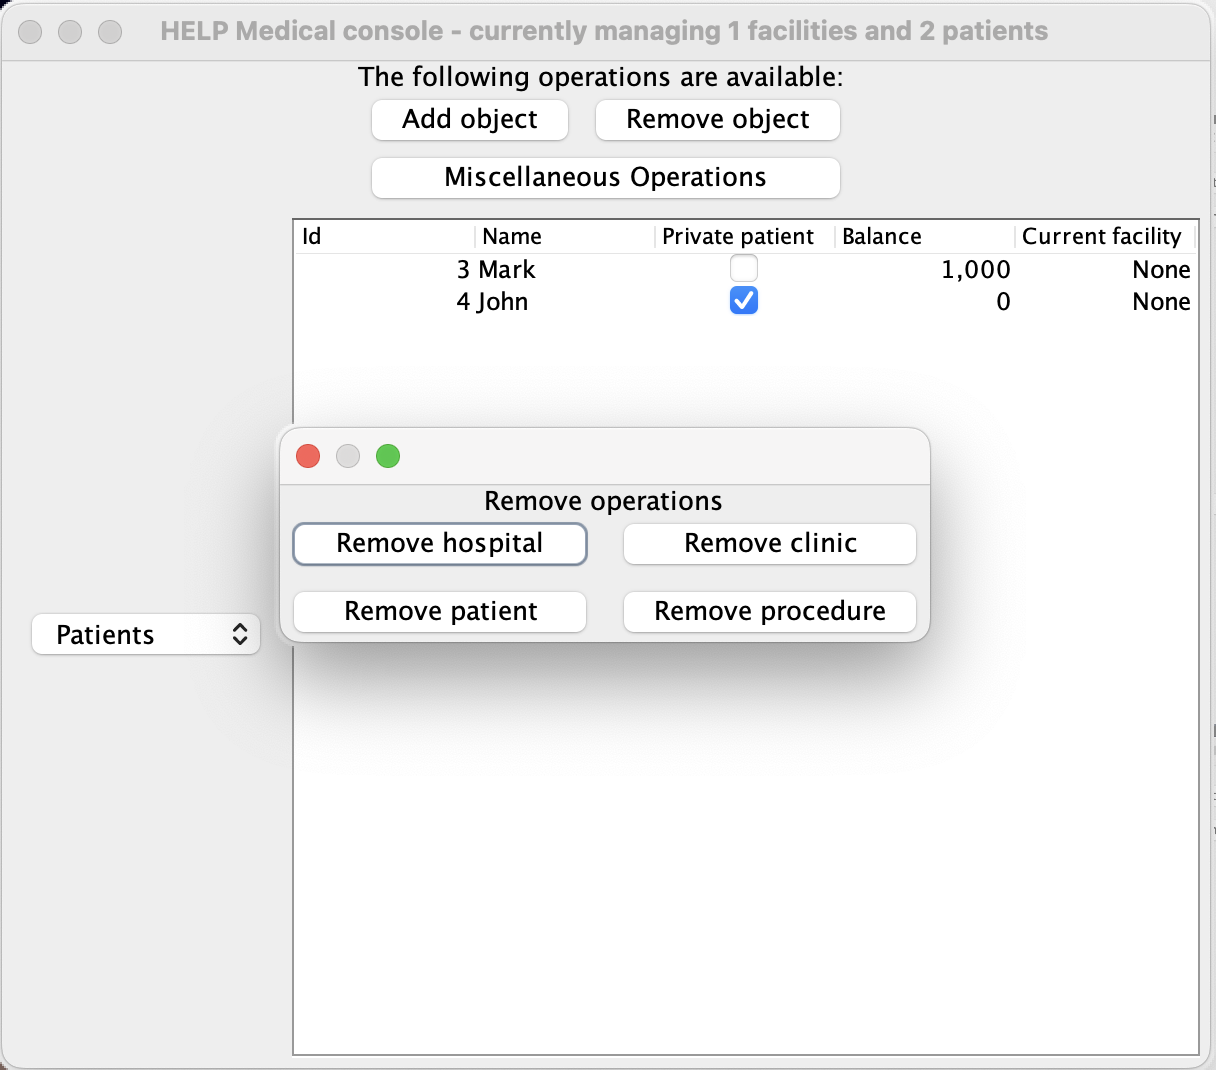
\includegraphics[width=0.5\textwidth]{./figures/Remove/Patient_1.png}
  \end{center}
\end{figure}

\begin{figure}
  \begin{center}
  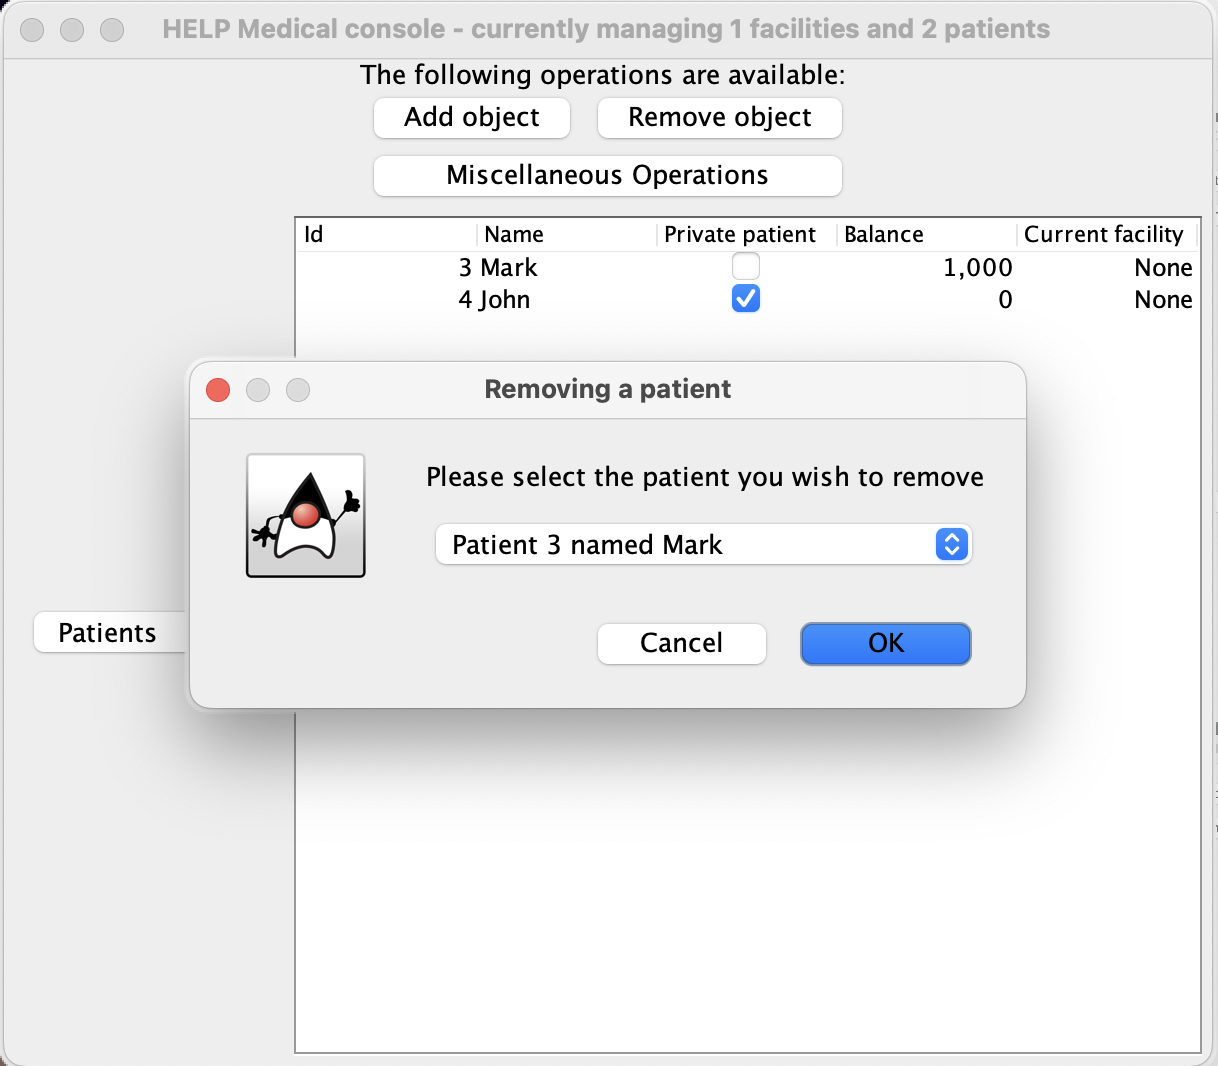
\includegraphics[width=0.5\textwidth]{./figures/Remove/Patient_2.png}
  \end{center}
\end{figure}

\begin{figure}
  \begin{center}
  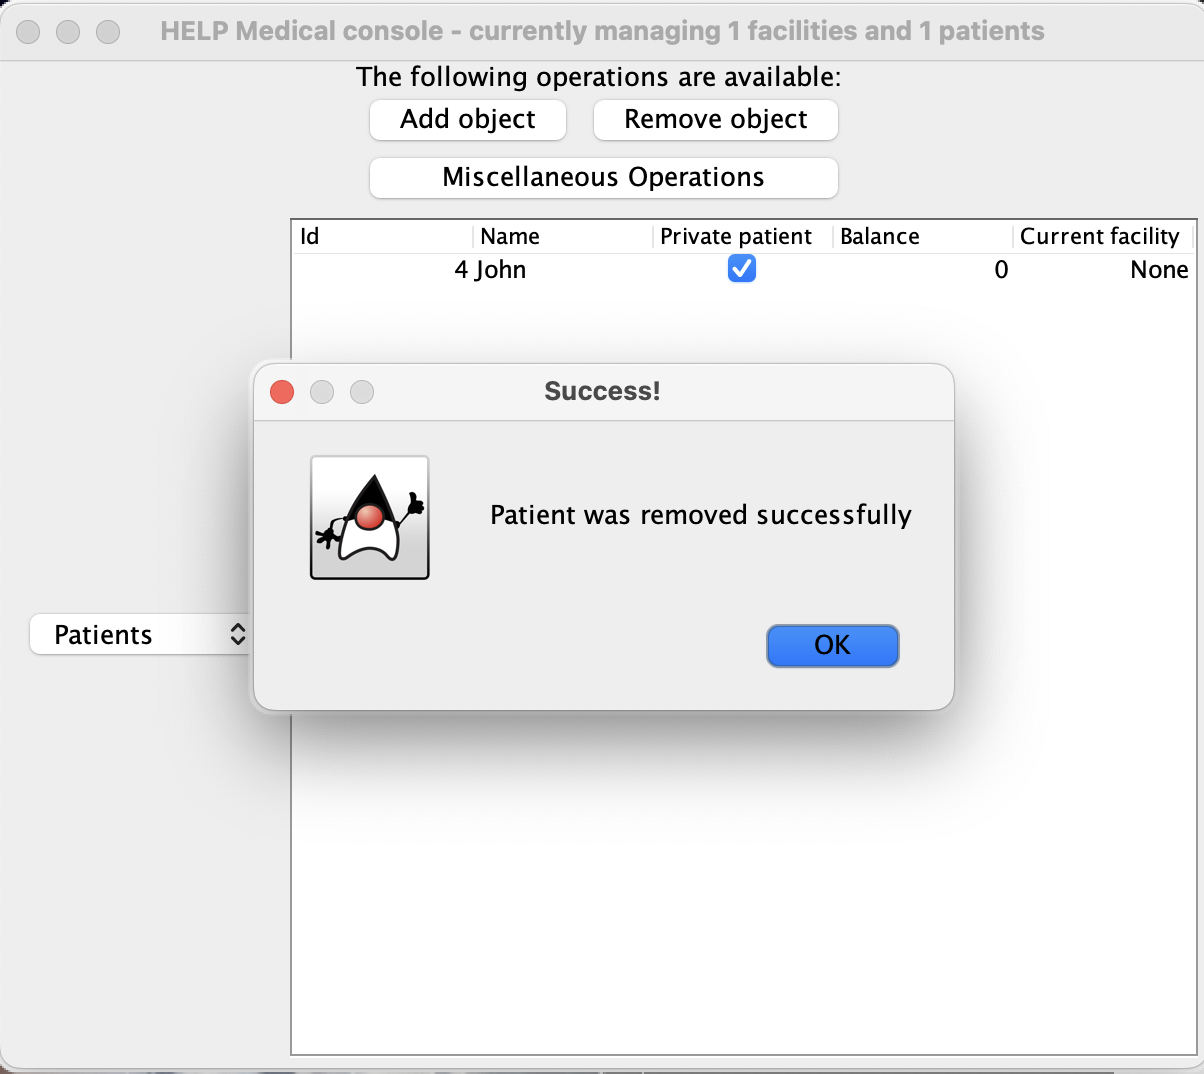
\includegraphics[width=0.5\textwidth]{./figures/Remove/Patient_3.png}
  \end{center}
\end{figure}

\begin{figure}
  \begin{center}
  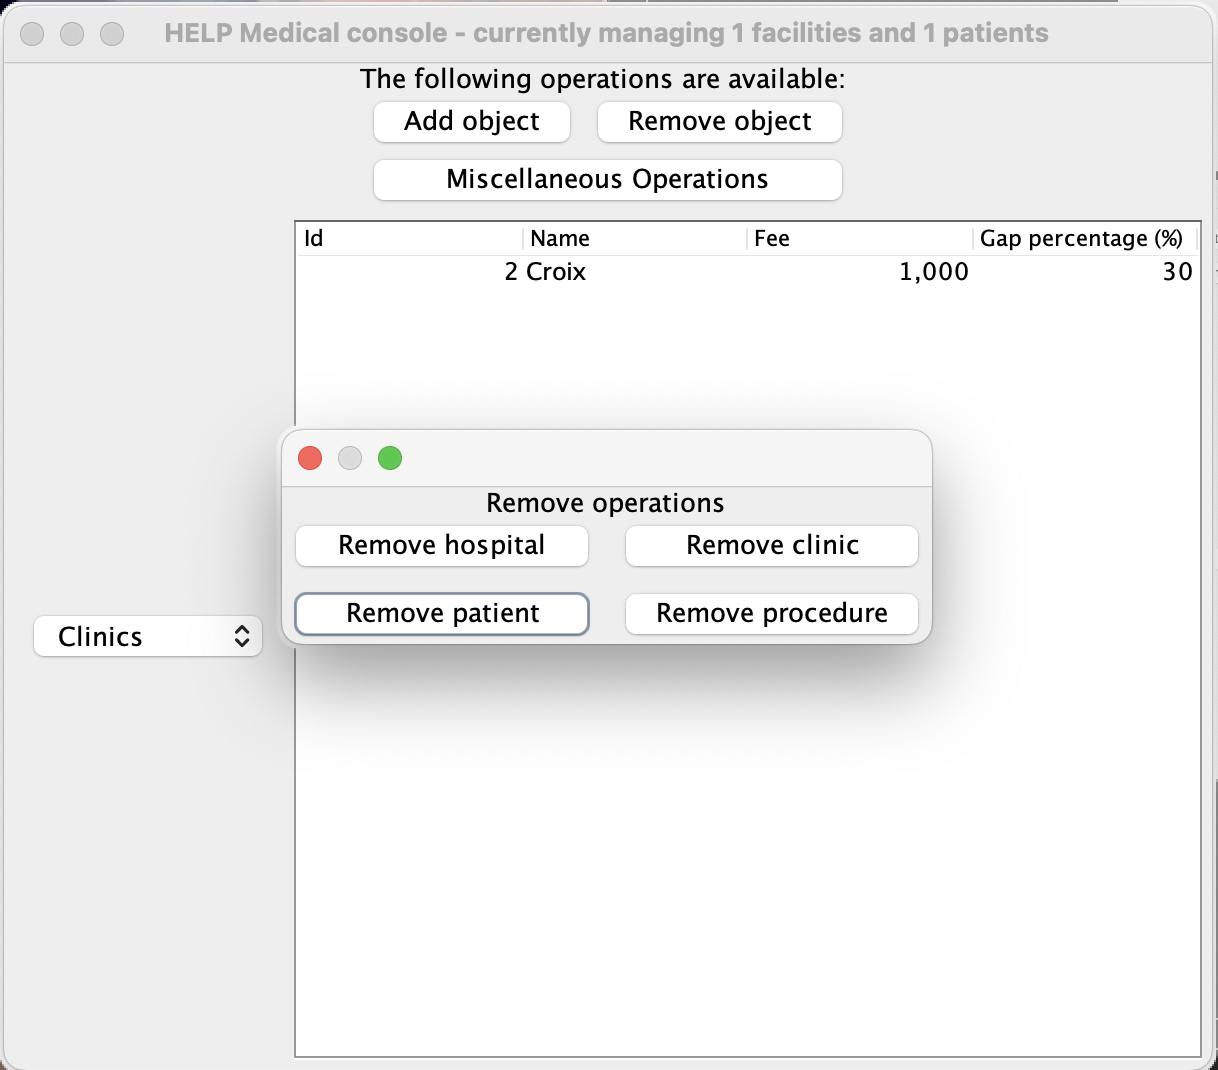
\includegraphics[width=0.5\textwidth]{./figures/Remove/Clinic_1.png}
  \end{center}
\end{figure}

\begin{figure}
  \begin{center}
    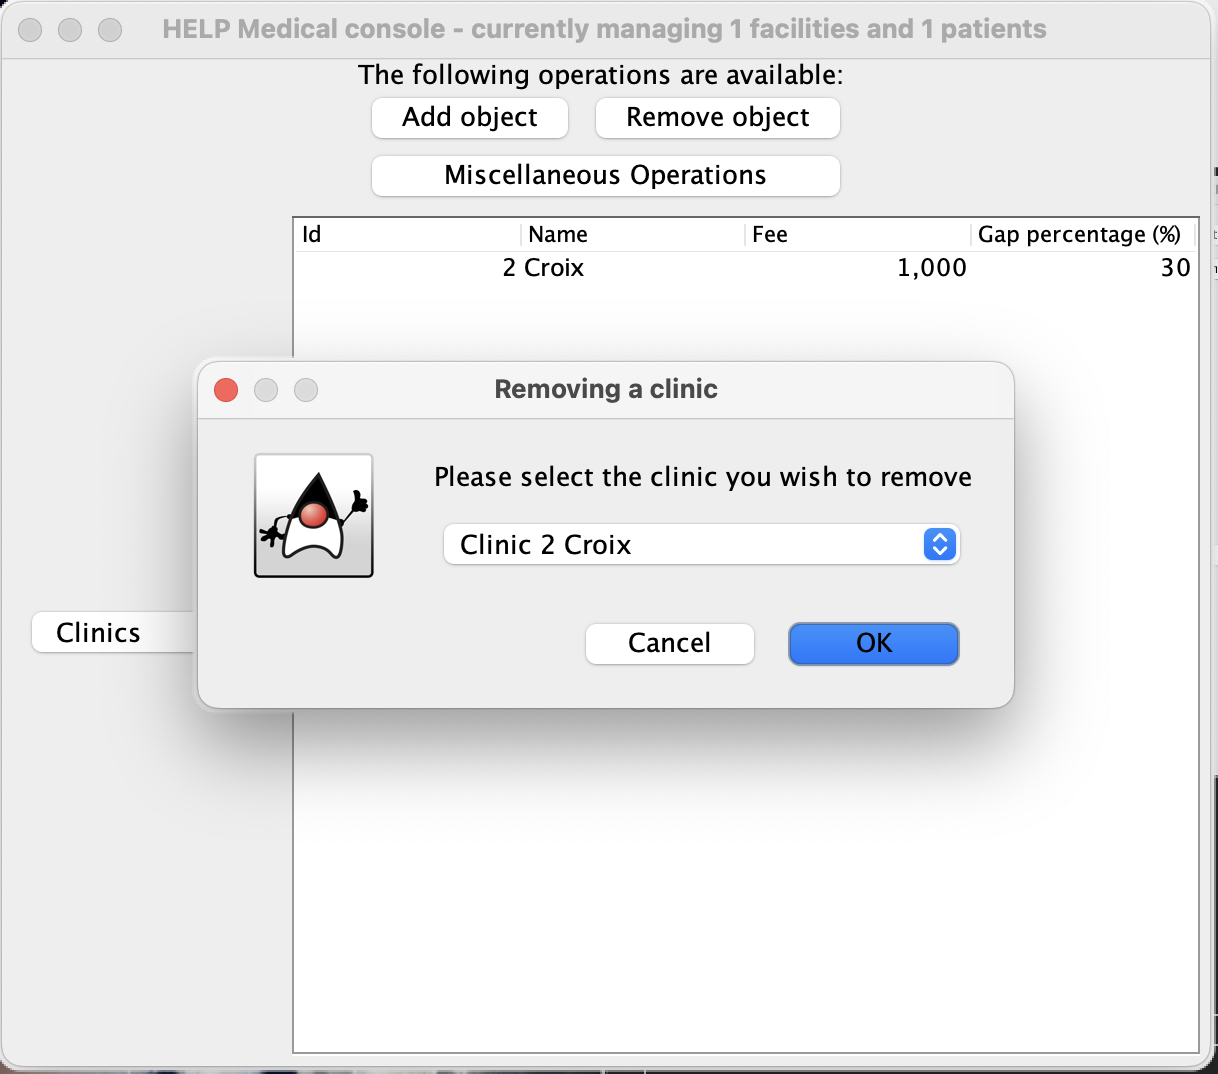
\includegraphics[width=0.5\textwidth]{./figures/Remove/Clinic_2.png}
  \end{center}
\end{figure}

\begin{figure}
  \begin{center}
  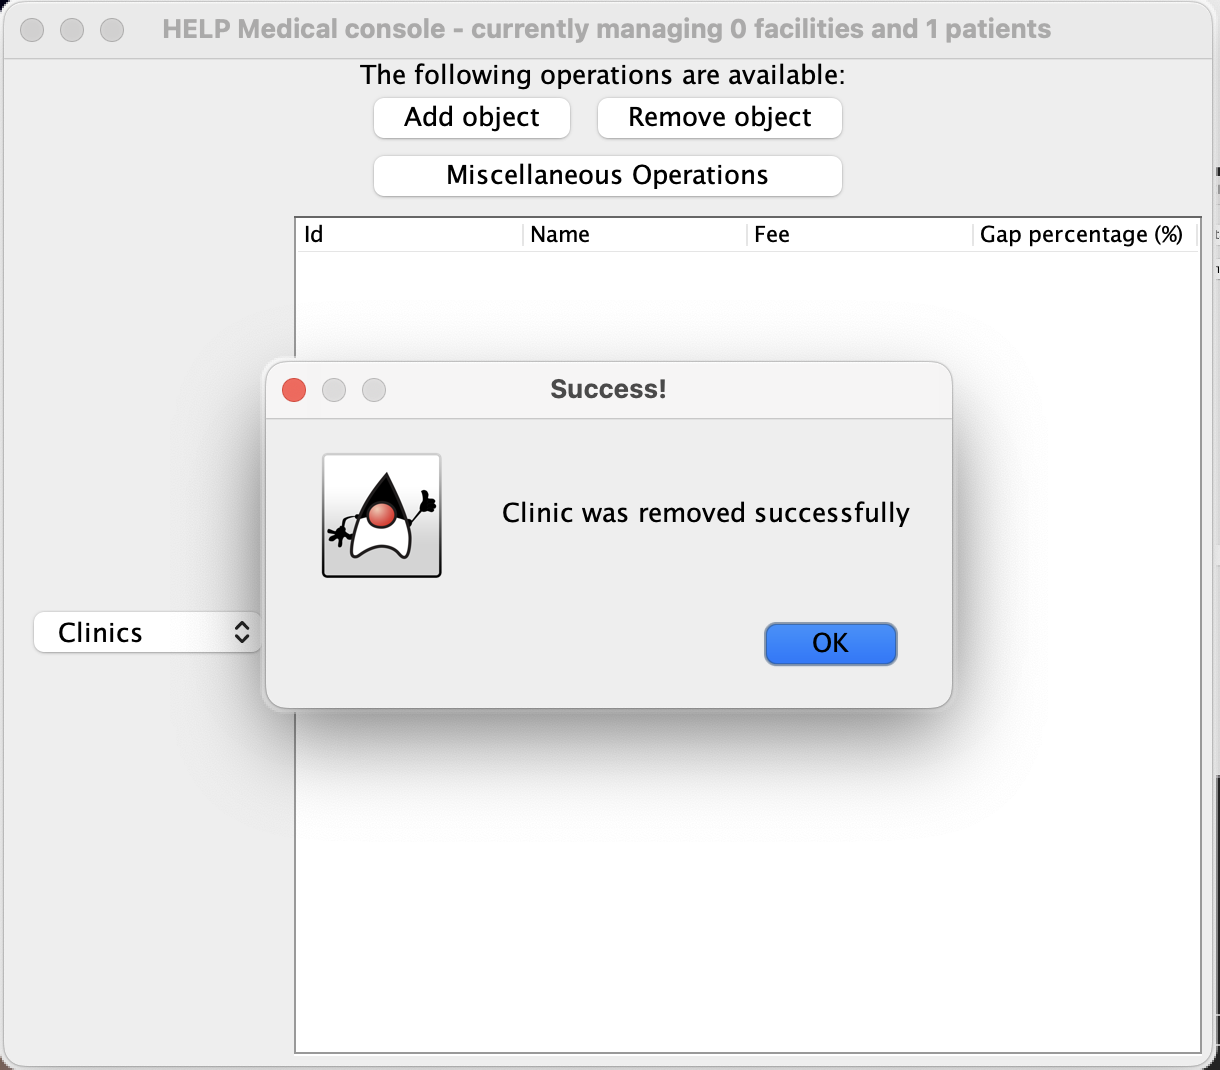
\includegraphics[width=0.5\textwidth]{./figures/Remove/Clinic_3.png}
  \end{center}
\end{figure}

\begin{figure}
  \begin{center}
    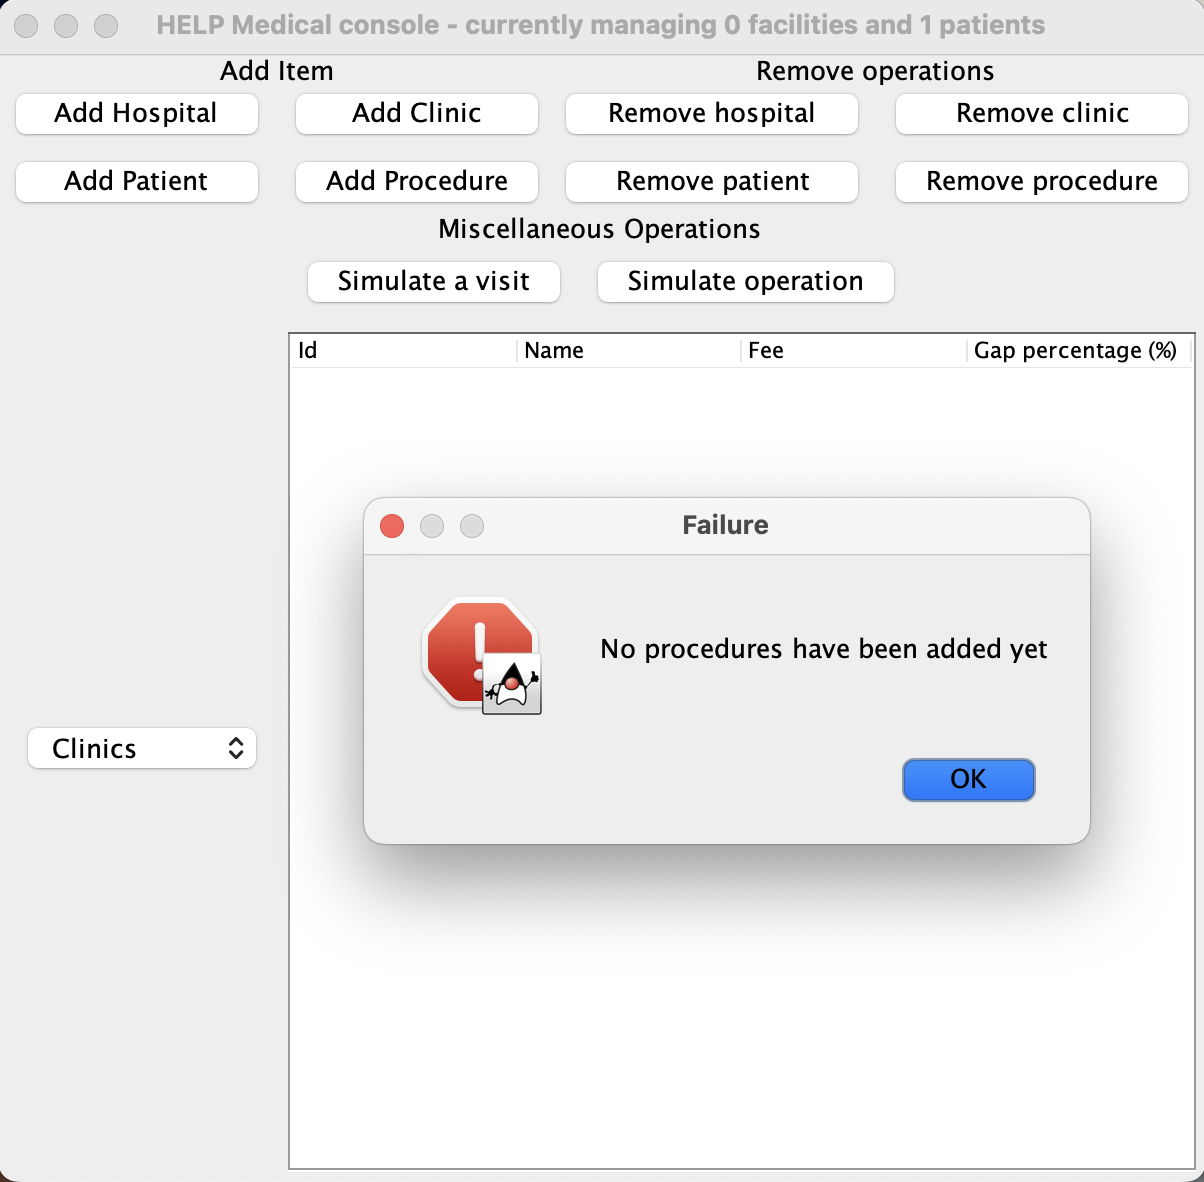
\includegraphics[width=0.5\textwidth]{./figures/Remove/Procedures_1.png}
  \end{center}
\end{figure}

The application also warns us if objects of a certain type have not been added yet. As is the case in the picture above.
% subsection Removing (end)

\subsection{Visiting}\label{sub:visiting} % (fold)
\begin{figure}
  \begin{center}
    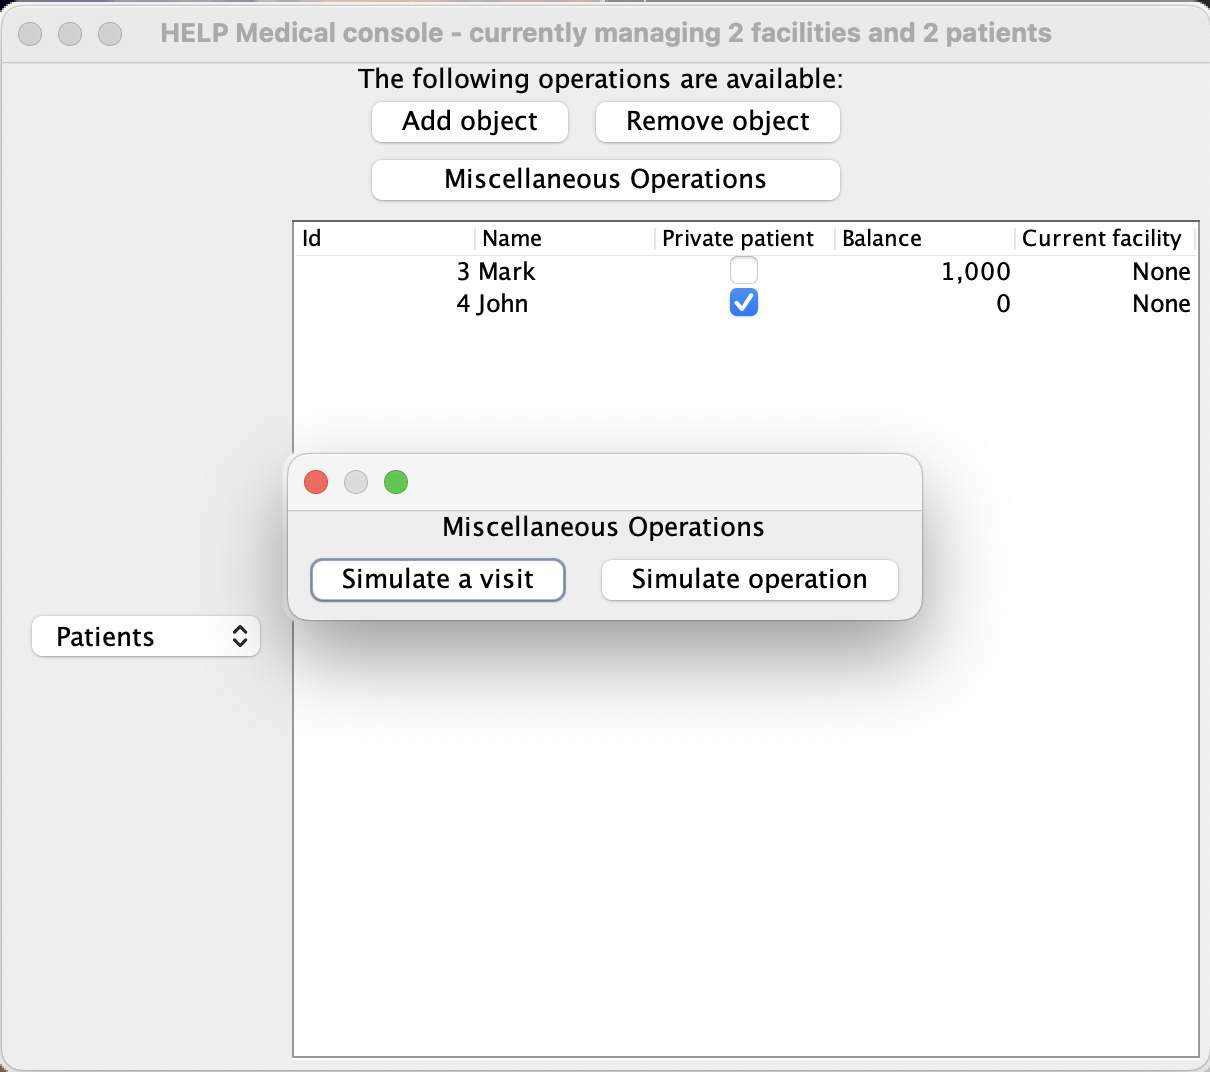
\includegraphics[width=0.5\textwidth]{./figures/Visit/Visit_1.png}
  \end{center}
\end{figure}

\begin{figure}
  \begin{center}
    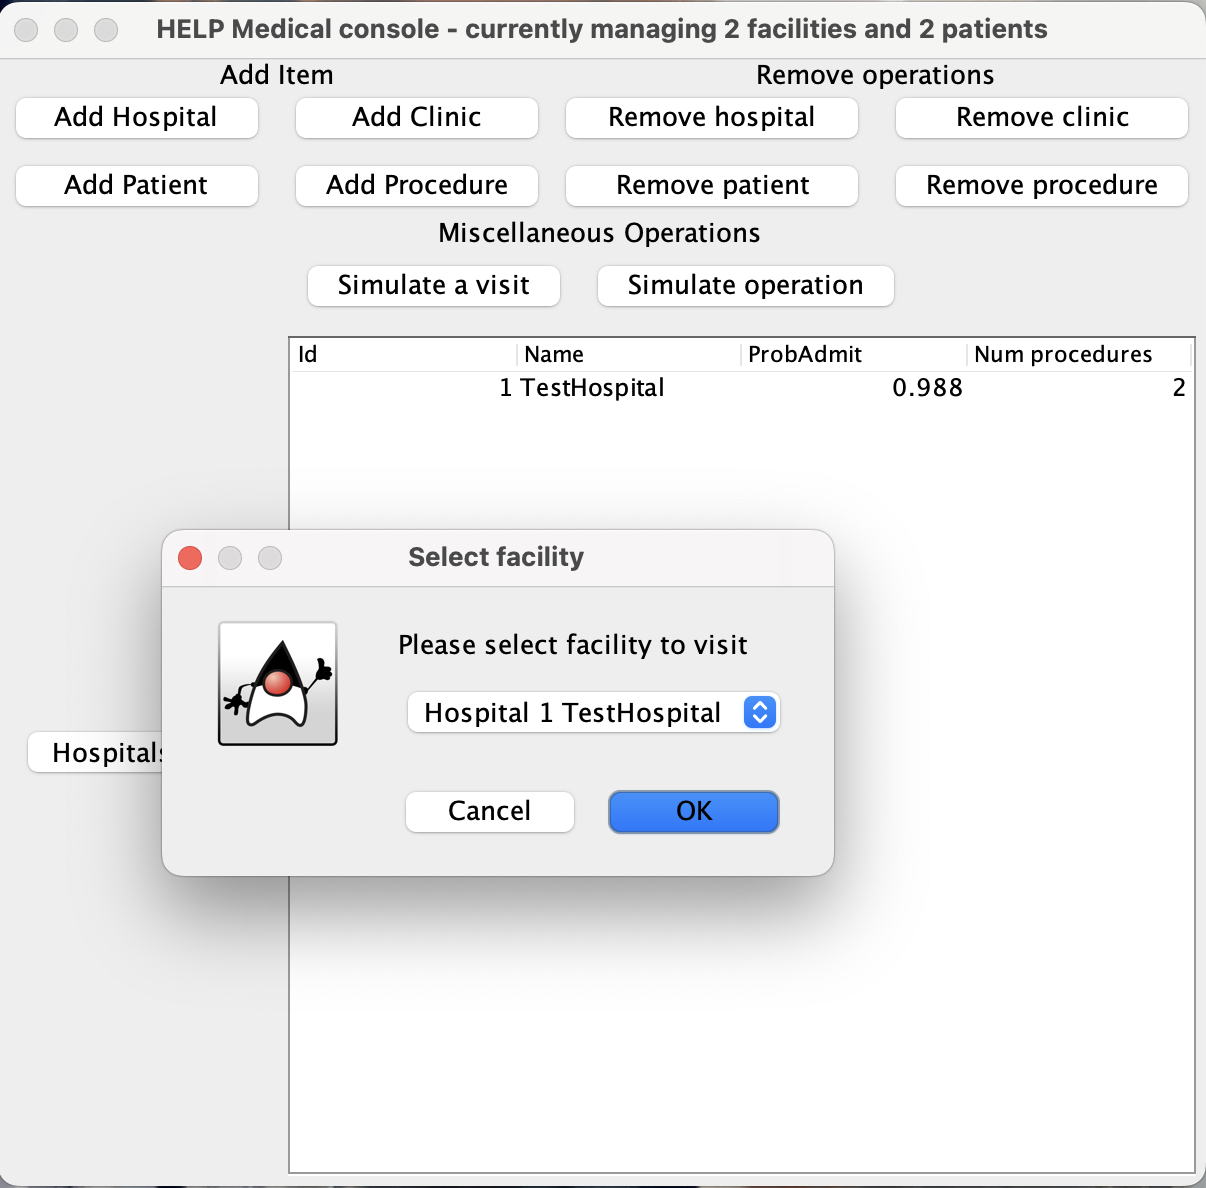
\includegraphics[width=0.5\textwidth]{./figures/Visit/Visit_2.png}
  \end{center}
\end{figure}

\begin{figure}
  \begin{center}
    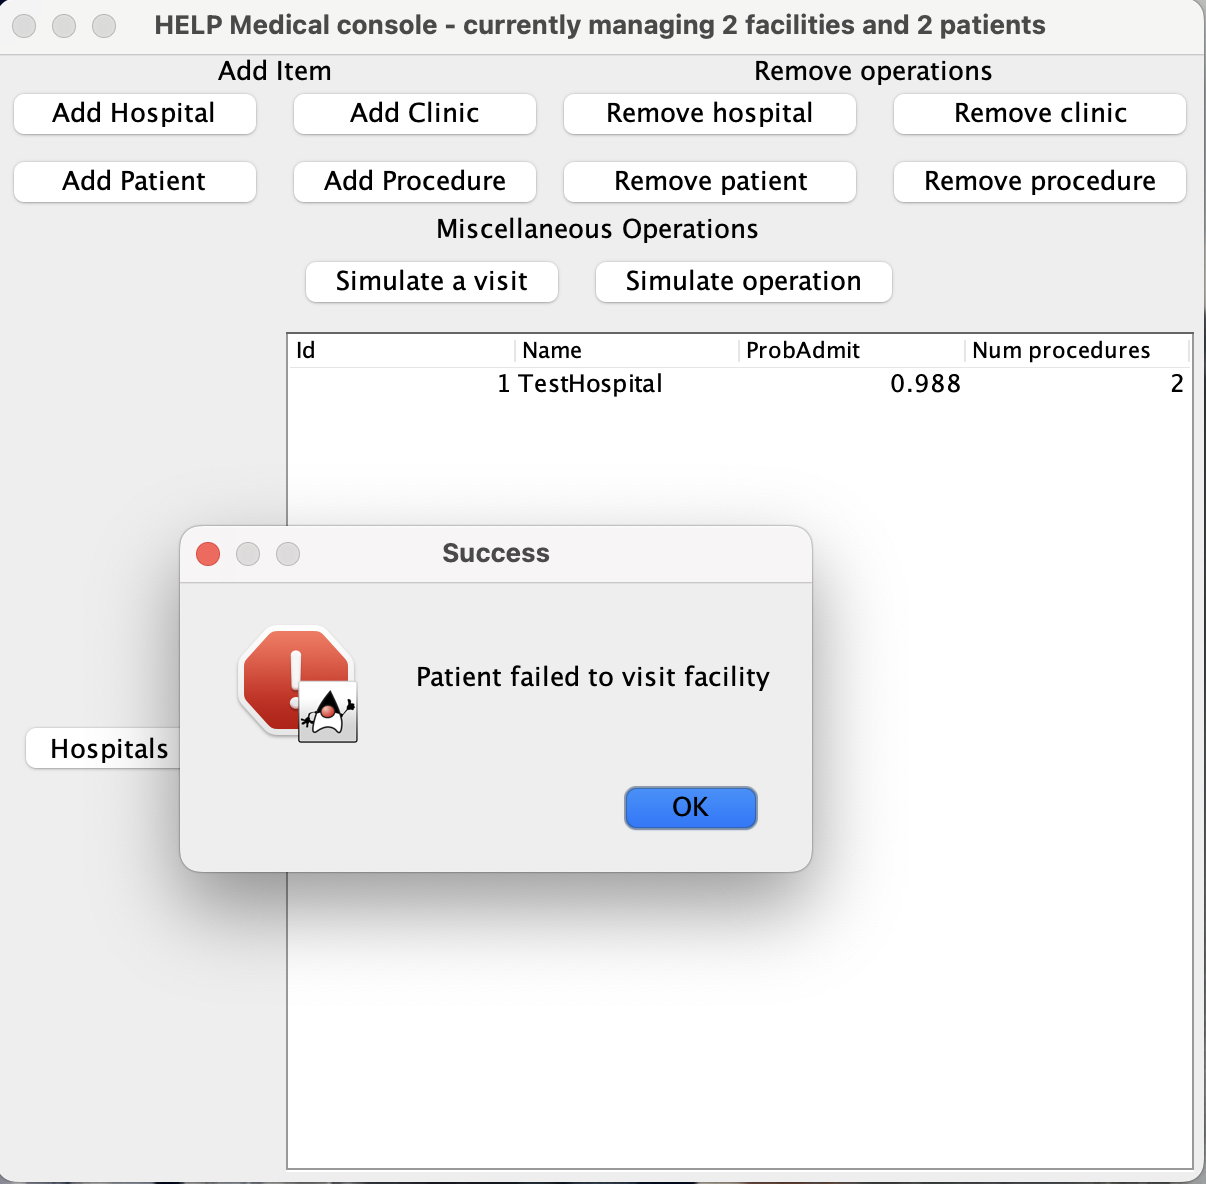
\includegraphics[width=0.5\textwidth]{./figures/Visit/Visit_3.png}
  \end{center}
\end{figure}
% subsection Visiting (end)

\subsection{Operating}\label{sub:operating} % (fold)
\begin{figure}
  \begin{center}
    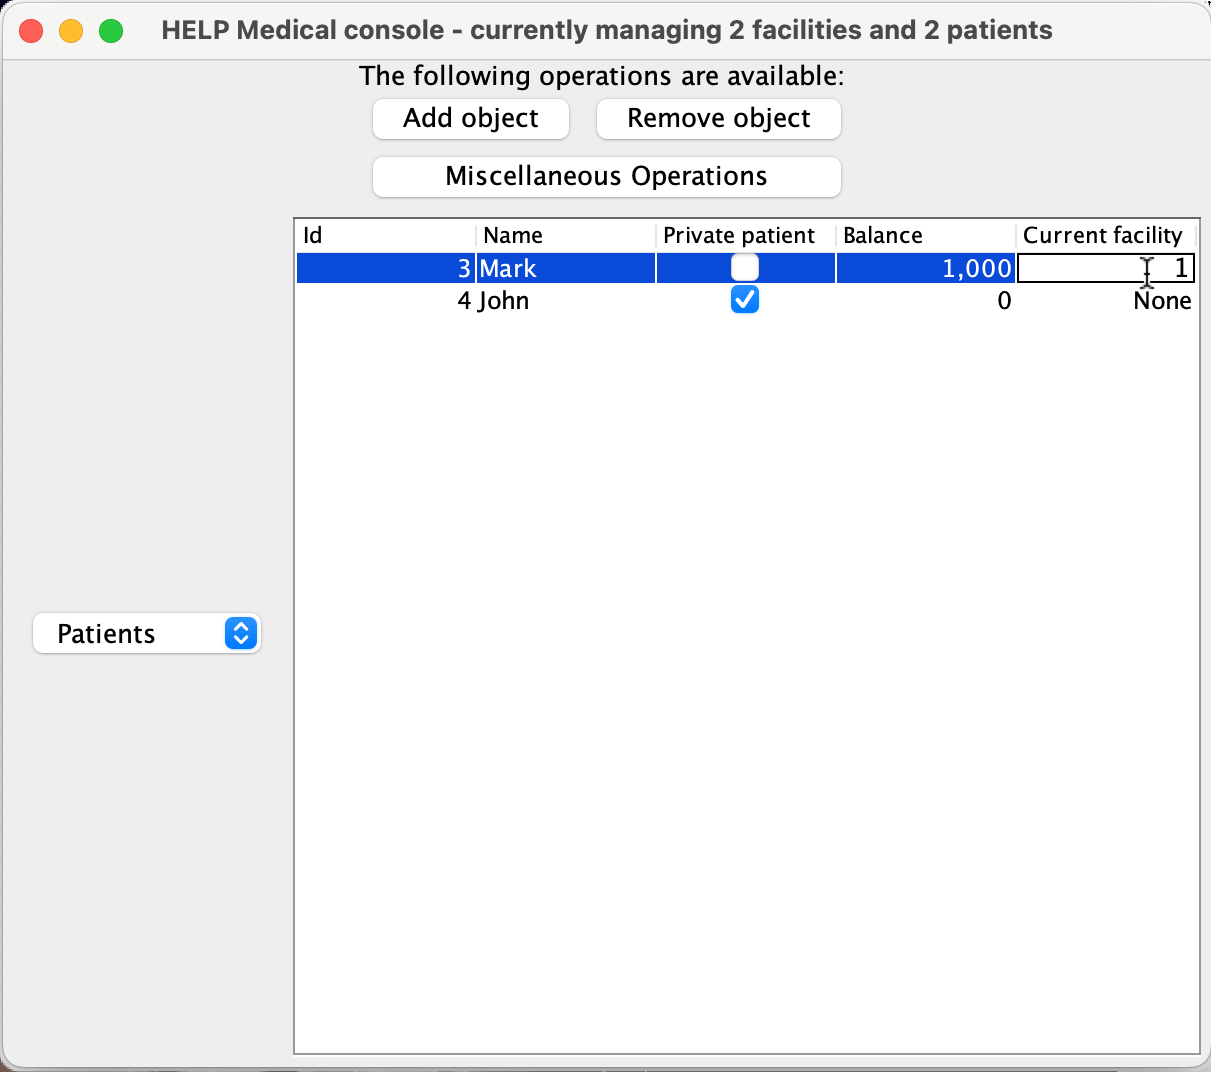
\includegraphics[width=0.5\textwidth]{./figures/Operation/Operation_1.png}
  \end{center}
\end{figure}

\begin{figure}
  \begin{center}
    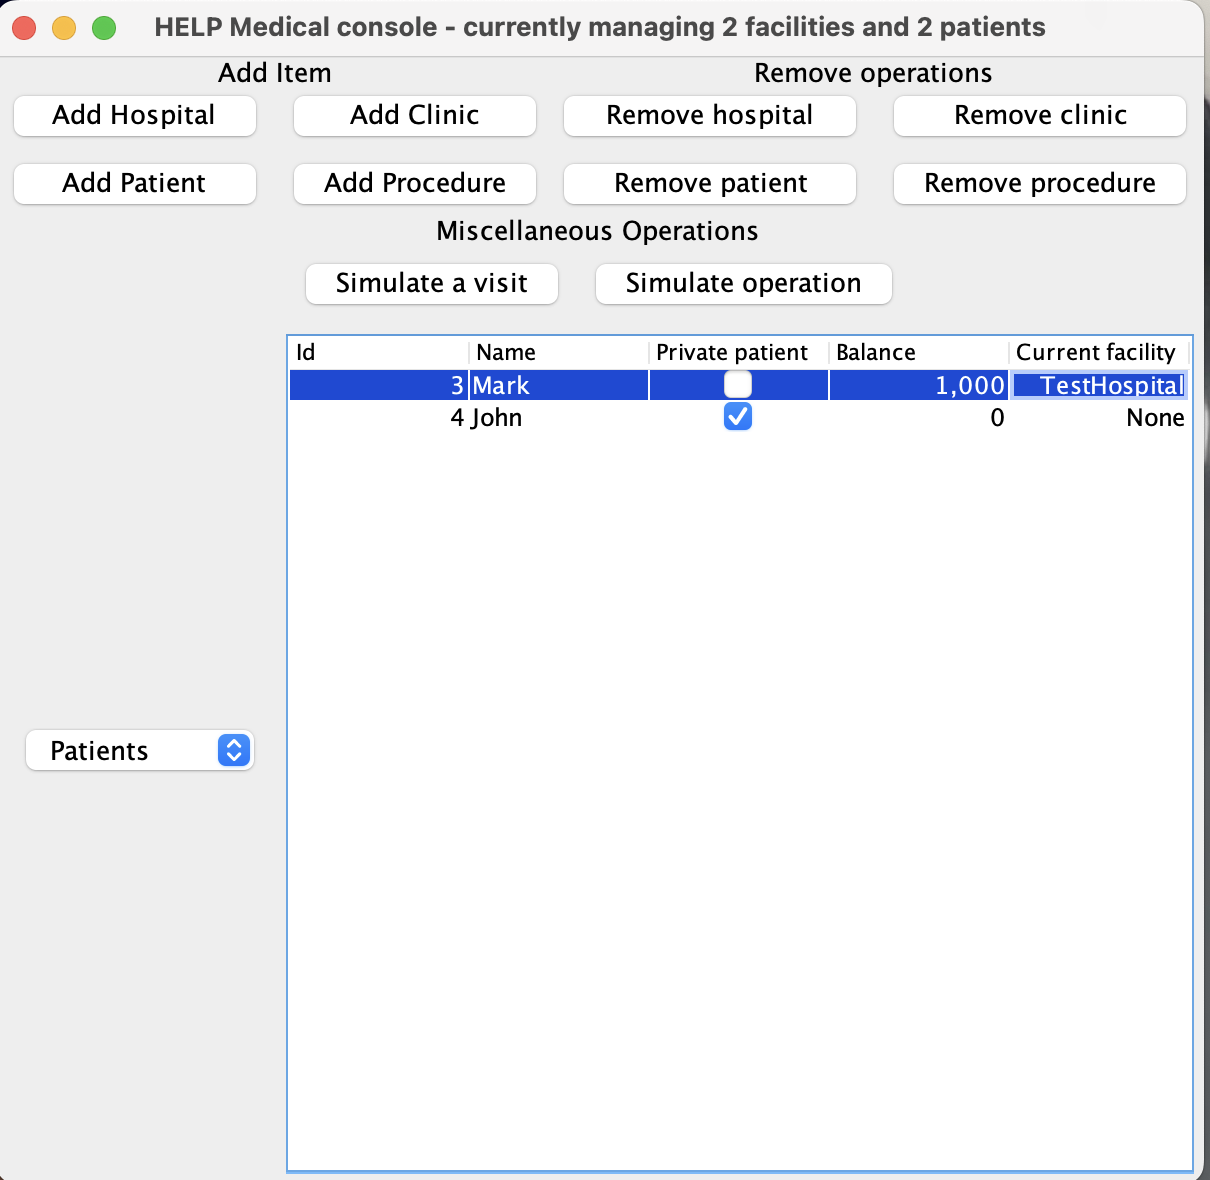
\includegraphics[width=0.5\textwidth]{./figures/Operation/Operation_2.png}
  \end{center}
\end{figure}

As can be seen from the $2$ previous pictures, the current facility of a patient can be directly edited. All records (except id) of all objects can be edited directly as well. Furthermore, if input is incorrect, the cell will prevent changes.

\begin{figure}
  \begin{center}
    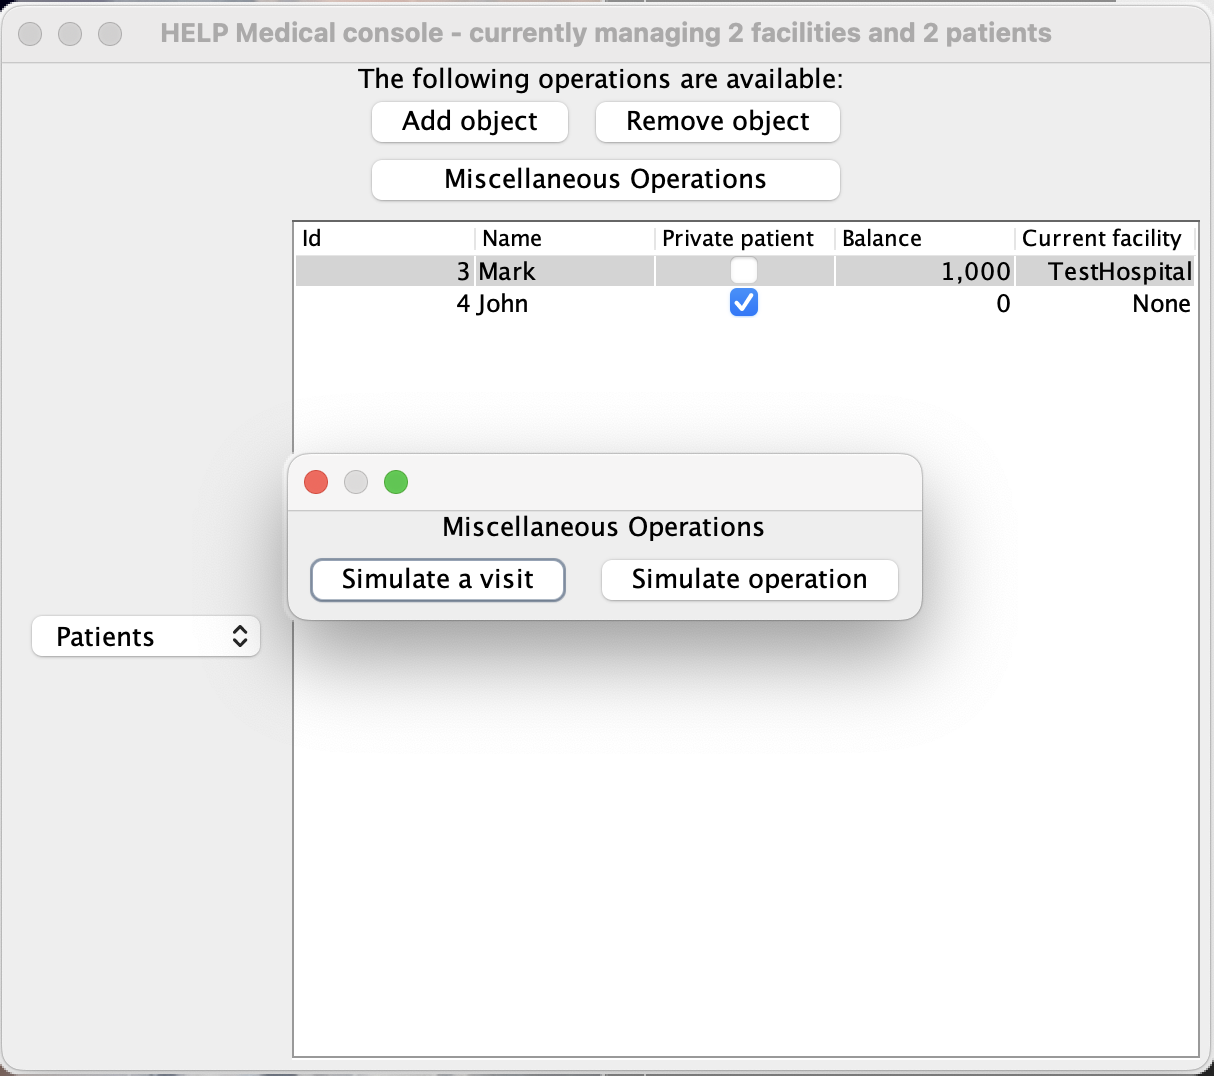
\includegraphics[width=0.5\textwidth]{./figures/Operation/Operation_3.png}
  \end{center}
\end{figure}

\begin{figure}
  \begin{center}
    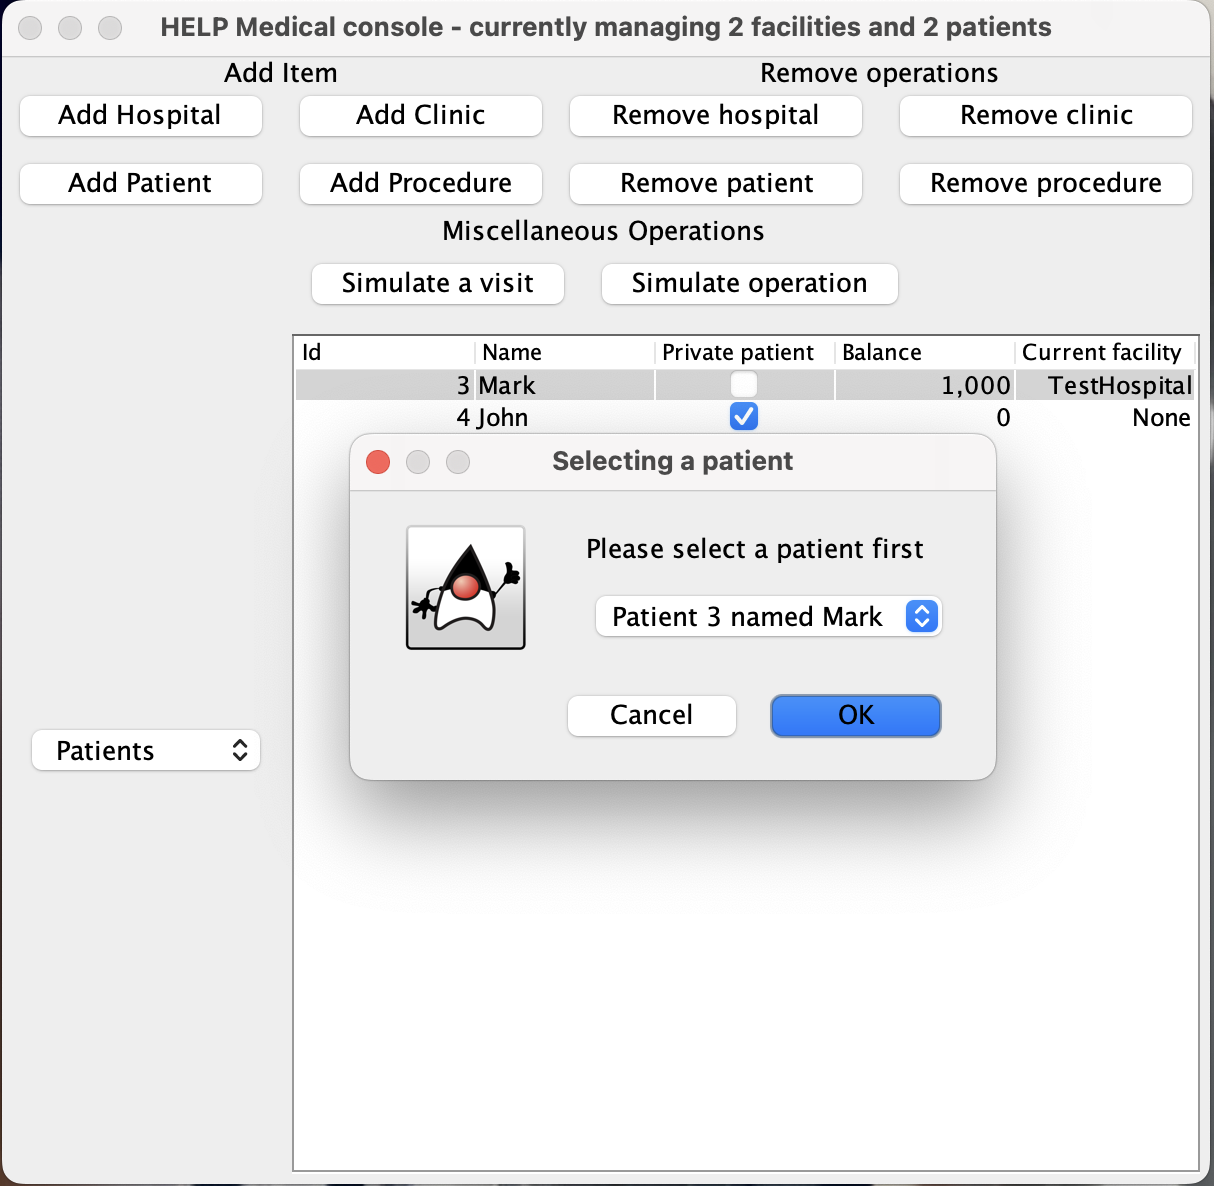
\includegraphics[width=0.5\textwidth]{./figures/Operation/Operation_4.png}
  \end{center}
\end{figure}

\begin{figure}
  \begin{center}
    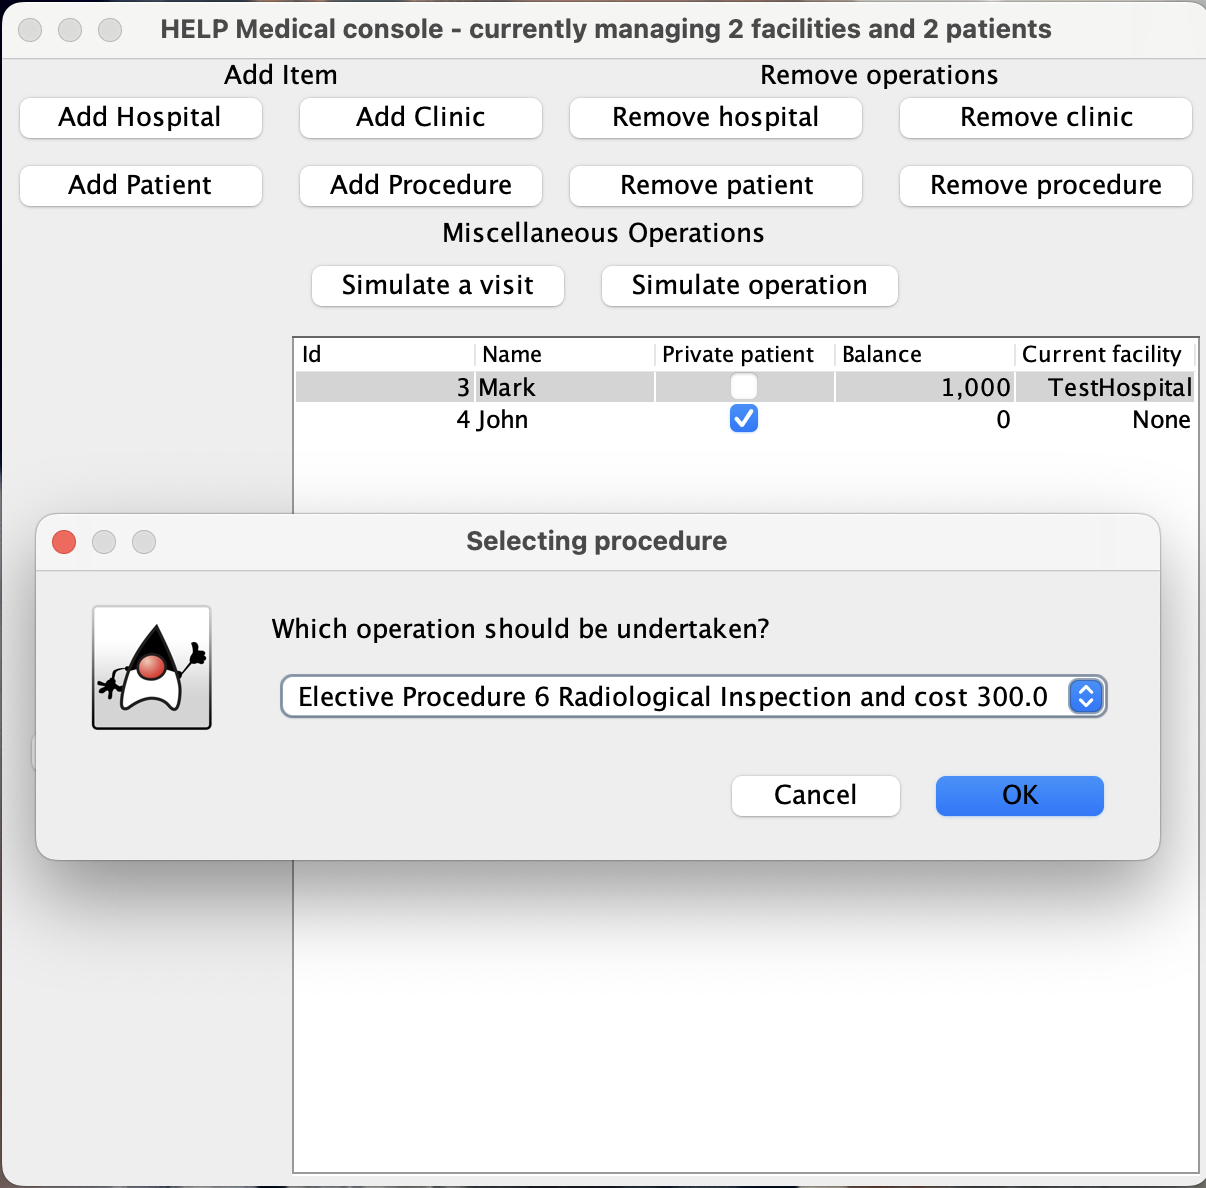
\includegraphics[width=0.5\textwidth]{./figures/Operation/Operation_5.png}
  \end{center}
\end{figure}

\begin{figure}
  \begin{center}
    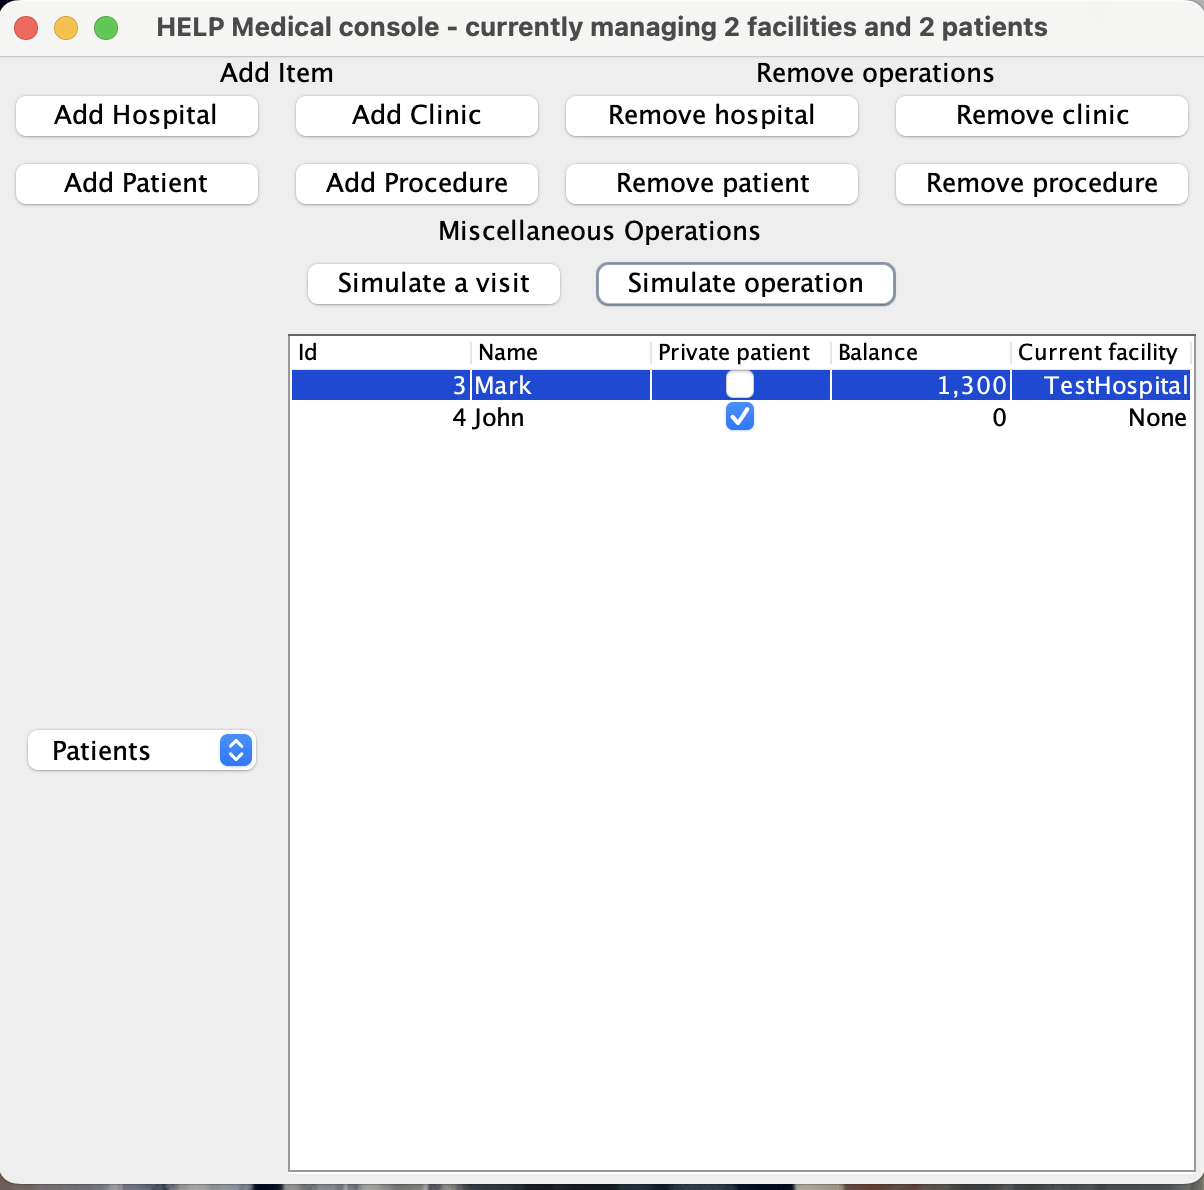
\includegraphics[width=0.5\textwidth]{./figures/Operation/Operation_6.png}
  \end{center}
\end{figure}

This balance is correct as the patient is public, and the procedure is elective, only the cost of the procedure is added to the balance, that is: 

\[
  1000 + 300 = 1300
\]
% subsection Operating (end)

\subsection{Saving}\label{sub:saving} % (fold)
The saving and loading menu uses the native system bar on MacOS, thanks to the check in \ref{MedicalGui.java}\cite{macos_titlebar}
\begin{figure}[ht]
  \begin{center}
    \includegraphics[width=0.7\textwidth]{figures/Save/Save_1.png}
  \end{center}
\end{figure}

\begin{figure}[ht]
  \begin{center}
    \includegraphics[width=0.7\textwidth]{figures/Save/Save_2.png}
  \end{center}
\end{figure}
% subsection Saving (end)

\subsection{Loading}\label{sub:loading} % (fold)
\begin{figure}[ht]
  \begin{center}
    \includegraphics[width=0.7\textwidth]{figures/Load/Load_1.png}
  \end{center}
\end{figure}

\begin{figure}[ht]
  \begin{center}
    \includegraphics[width=0.7\textwidth]{figures/Load/Load_2.png}
  \end{center}
\end{figure}

\begin{figure}[ht]
  \begin{center}
    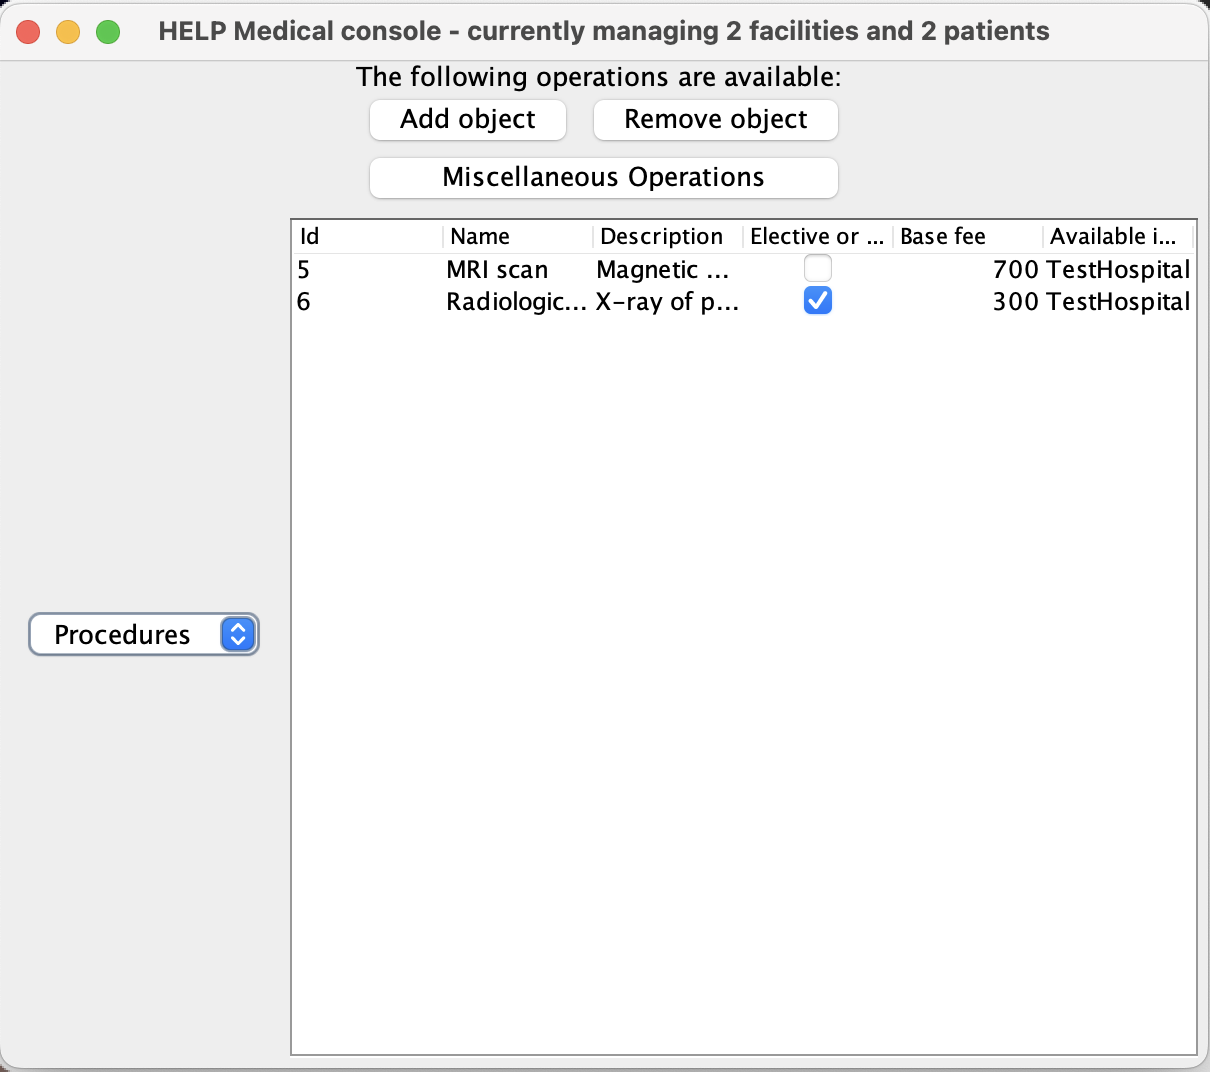
\includegraphics[width=0.7\textwidth]{figures/Load/Load_3.png}
  \end{center}
\end{figure}

As can be seen from the picture above, this feature works properly as all objects are loaded back into the application, as seen by both the table, and the titlebar showing the right data.
% subsection Loading (end)
% section Runtime output (end)

\section{Bibliography}\label{sec:bibliography} % (fold)
\printbibliography

% section Bibliography (end)
\end{document}
